\documentclass[10pt,openany]%,oneside]
{book}

\newcommand{\versiondate}[0]{Aug 2, 2022}


\usepackage{
  amsmath, calc,
  caption, changepage,
  endnotes, enumerate,
  fancyhdr,
  fix-cm,
  fncychap,
  footmisc,
  fullminipage,
  geometry, graphicx,  
  ifthen, lscape,
  makeidx, manfnt,
  marginnote,
  mdframed,
  multicol, multirow,
  setspace, soul,
  tabto,
  textcomp,
  %tocloft,
  varioref, verbatim,
  wasysym, wrapfig}
\usepackage{epstopdf}
\usepackage{subfigure}
\usepackage[explicit]{titlesec}
%\usepackage[usenames,dvipsnames]{color}  
%\newcommand{\href}[2]{#2} \newcommand{\url}[1]{#1} \newcommand{\urlstyle}[1]{}

\definecolor{oiGA}{rgb}{0,0,0}
\definecolor{oiGB}{rgb}{.5,.5,.5}
\definecolor{oiGC}{rgb}{.85,.85,.85}
\definecolor{oiB}{rgb}{.365,.529,.631}
%\definecolor{oiB}{rgb}{0,0,0}
\definecolor{oiG}{rgb}{.298,.447,.114}
\definecolor{oiY}{rgb}{.957,.863,0}
\definecolor{oiR}{rgb}{.941,.318,.200}
\definecolor{redcards}{rgb}{.941,.318,.200}


\definecolor{rd}{rgb}{.80,.0,.0}
\definecolor{tableHL}{rgb}{.5,.1,.2}
\definecolor{tableHLBlue}{rgb}{.2,.4,.9}
\definecolor{highlight}{rgb}{.5,.1,.2}
\definecolor{highlightO}{rgb}{.1,.3,.8}
\definecolor{highlightT}{rgb}{.6,.3,.1}
\definecolor{ex}{rgb}{.0,.30,.55}
\definecolor{gray}{rgb}{.5,.5,.5}
\definecolor{chaptertitlegray}{rgb}{.5,.5,.5}
\definecolor{steelBlue}{rgb}{.3,.4,.8}
\definecolor{excolor}{rgb}{.0,.3,.55}
\definecolor{secolor}{rgb}{.0,.3,.55}
\definecolor{comment}{rgb}{.65,.45,.25}
\definecolor{grayDark}{rgb}{.43,.43,.43}
\definecolor{grayLight}{rgb}{.65,.65,.65}
\definecolor{grayBackground}{rgb}{.92,.92,.92}
\definecolor{seaBackground}{rgb}{.851,.894,.867}
\definecolor{examplegray}{rgb}{0,0,0} %{.83,.83,.83}
\definecolor{termOColor}{rgb}{.65,.1,.1}


\newcommand{\printlocation}[0]{}

\newcommand{\chapterpagepadding}[0]{7mm}
\newcommand{\chapterpagepaddingleftright}[0]{\chapterpagepadding{}}
\newcommand{\chapterpagepaddingleftinner}[0]{25mm}
\newcommand{\chapterpagepaddingrightinner}[0]{30mm}

% _____ (1) PDF _____ %
\usepackage[bookmarksnumbered, colorlinks = false, pdfborder = {0 0 0}, urlcolor = oiGB, colorlinks=true, linkcolor = oiGB, citecolor = oiGB, backref = true]{hyperref}

% _____ (2) PDF -- screenreader _____ %
%\usepackage{pdfcomment}
% !!!!!
% 1. Use the `style_simple` instead of `style`.
% 2. Use the `headers_simple` instead of `headers`.
% 3. Adjust the TOC depth to 3.
% !!!!!

% _____ (3) B&W Paperback _____ %
%\definecolor{oiB}{rgb}{0,0,0}\definecolor{chaptertitlegray}{rgb}{0,0,0}\PassOptionsToPackage{hyperref}{colorlinks=false,pdfborder={0 0 0},urlcolor= black,colorlinks=black,linkcolor=black, citecolor=black,backref=true}

% _____ (4) Hardcover _____ %
%\definecolor{oiB}{rgb}{0,0,0}\definecolor{chaptertitlegray}{rgb}{0,0,0}\PassOptionsToPackage{hyperref}{colorlinks=false,pdfborder={0 0 0},urlcolor= black,colorlinks=black,linkcolor=black, citecolor=black,backref=true}
% !!!!!
% Also must \include{extraTeX/style/hardcover} below.
% !!!!!
% \renewcommand{\printlocation}[0]{\noindent Printed in China. \\}

% _____ (5) Color Paperback _____ %
%\definecolor{chaptertitlegray}{rgb}{0,0,0}\usepackage[bookmarksnumbered, pdfborder = {0 0 0}, urlcolor = black, colorlinks=true, linkcolor = black, citecolor = black, backref = true]{hyperref}\renewcommand{\chapterpagepaddingleftright}[0]{15mm} \renewcommand{\chapterpagepaddingleftinner}[0]{17mm}\renewcommand{\chapterpagepaddingrightinner}[0]{22mm}




\usepackage[style=authortitle-ibid, maxnames=2,natbib=true,sortcites=true,block=space,backend=bibtex]{biblatex}
\bibliography{eoce.bib}

\makeindex
% 1 Page Parameters
% 2 Special Commands for Editions
% 3 Content Modifications
% 4 Counters and Parameters
% 5 Section Coloring
% 6 Utilities
% 7 
% 8 Figures and Captions
% 9 Examples and Exercises
% 10 Special Boxes

%\renewcommand\chapter{\if@openright\cleardoublepage\else\clearpage\fi
%                    \thispagestyle{fancy}%
%                    \global\@topnum\z@
%                    \@afterindentfalse
%                    \secdef\@chapter\@schapter}
\fancypagestyle{plain}{%
\fancyhf{} % clear all header and footer fields
\fancyhead[RO,RE]{\thepage} %RO=right odd, RE=right even
\renewcommand{\headrulewidth}{0pt}
\renewcommand{\footrulewidth}{0pt}}
\raggedbottom


\newcommand{\stdspace}[0]{3mm}
\newcommand{\stdvspace}[0]{\vspace{\stdspace{}}}
\newcommand{\stdaddvspace}[0]{\addvspace{\stdspace{}}}




%-------------------------------------------------------------
% 1 Page Parameters
% 1.1
\setlength\paperheight{11in}
\setlength\paperwidth{8.5in}
\newcommand{\officialtextheight}{9.7in}
\newcommand{\officialtextwidth}{6in}
%\setlength\paperheight{10in}
%\setlength\paperwidth{8in}
%\newcommand{\officialtextheight}{8.7in}
%\newcommand{\officialtextwidth}{6in}
\newcommand{\officialvoffset}{-0.6in}
\setlength\textheight{\officialtextheight}
\setlength\textwidth{\officialtextwidth}
\setlength\voffset{\officialvoffset}
\renewcommand{\baselinestretch}{1.0}
% 1.2 Margin Size
% 1.2.1 Slim
%\setlength\hoffset{0.25in}
%\setlength\oddsidemargin{0.25in}
%\setlength\evensidemargin{0in}
% 1.2.2 Medium
\setlength\hoffset{3.7mm}
\setlength\oddsidemargin{3mm}
\setlength\evensidemargin{3mm}
% 1.2.3 Wide
%\setlength\hoffset{-5mm}
%\setlength\oddsidemargin{0.5in}
%\setlength\evensidemargin{0.5in}
% 1.3 PDF Parameters
%\setlength\paperheight{11in}
%\setlength\textheight{8.25in}
%\setlength\paperwidth{8.5in}
%\setlength\textwidth{5.45in}
%\setlength\voffset{-10mm}
%\setlength\oddsidemargin{0.75in}
%\setlength\evensidemargin{0.75in}
% 1.4 Margin Spacing
\setlength{\marginparsep}{5mm}
\setlength{\marginparwidth}{20mm}
% 1.5 Page Header
\pagestyle{fancy}
\renewcommand{\headrulewidth}{0pt}
\fancyhead[RO,LE]{\thepage}
\fancyhead[RE]{\leftmark}
\fancyhead[LO]{\rightmark}
\fancyfoot[c]{}
\fancyheadoffset[RO,LE]{0.9in}



% Tablet Version
%\setlength\paperheight{8.82in}\setlength\textheight{8.25in}\setlength\paperwidth{5.7in}\setlength\textwidth{5.45in}\setlength\voffset{-23.5mm}\setlength\hoffset{-27mm}\setlength\oddsidemargin{5mm}\setlength\evensidemargin{5mm}\setlength{\marginparsep}{5mm}\setlength{\marginparwidth}{35mm}\fancyheadoffset[RO,LE]{0.2in}




%-------------------------------------------------------------
% 2 Special Commands for Editions
\newcommand{\referrer}{AHSS2_pdf}
\newcommand{\vspaceB}[1]{}
\newcommand{\hspaceB}[1]{}
\newcommand{\textB}[1]{}
\newcommand{\textC}[1]{}
\newcommand{\B}[1]{#1}

\newcommand{\D}[1]{#1}



%-------------------------------------------------------------
% 3 Content Modifications
\newcommand{\APVersion}[2]{#2}
\newcommand{\MultipleRegression}[2]{#1}
\newcommand{\MultipleRegressionChapter}[2]{#1}
\newcommand{\SimulationAndRandomization}[1]{#1}
\newcommand{\ANOVASection}[2]{#1}
\newcommand{\GLMSection}[2]{#1}




%-------------------------------------------------------------
% 4 Counters and Parameters
% 4.1 Counters
\newcounter{alwaysOne}
\setcounter{alwaysOne}{1}
\newcounter{alwaysTwo}
\setcounter{alwaysTwo}{2}
\newcounter{alwaysThree}
\setcounter{alwaysThree}{3}
\newcounter{alwaysFour}
\setcounter{alwaysFour}{4}
\newcounter{withinChNum}[chapter]
\setcounter{withinChNum}{0}
\newcounter{eoce}[chapter]
\renewcommand{\theeoce}
    {\arabic{chapter}.\arabic{eoce}}
\newcounter{eocesolch}
\setcounter{eocesolch}{0}
\newcounter{eocesol}[eocesolch]
\renewcommand{\theeocesol}
     {\arabic{eocesolch}.\arabic{eocesol}}
\newcounter{eoceNeedSolution}[chapter]
\renewcommand{\theeoceNeedSolution}
    {\arabic{chapter}.\arabic{eoceNeedSolution}}
\newcounter{eoceReplace}[chapter]
\renewcommand{\theeoceReplace}
    {\arabic{chapter}.\arabic{eoceReplace}}
\newcounter{eoceFF}[chapter]
\renewcommand{\theeoceFF}
    {\arabic{chapter}.\arabic{eoceFF}}
% 4.2 Parameters
\newlength{\exampleAboveBar}
\newlength{\exampleBelowBar}
\setlength{\exampleAboveBar}{-3.15mm}
\setlength{\exampleBelowBar}{-1.15mm}
\newlength{\nexampleAboveBar}
\newlength{\nexampleBelowBar}
\setlength{\nexampleAboveBar}{-1mm}
\setlength{\nexampleBelowBar}{-1mm}
% 4.3 Chapter Declarations
\newcommand\includechapter[2]{
  \setcounter{chapter}{#1}
  \addtocounter{chapter}{-1}
  \normalsize
  \include{#2/TeX/#2}
  \newpage\reviewexercisesheader{}

% 39 - tf_correlation

\eoce{\qt{True / False\label{tf_correlation}}
Determine if the following statements are true or false.
If false, explain why.
\begin{parts}
\item A correlation coefficient of -0.90 indicates a stronger 
linear relationship than a correlation of 0.5.
\item Correlation is a measure of the association between any 
two variables.
\end{parts}
}{}

% 40 - cat_body_heart_inf_2s_ahss

\eoce{\qt{Cats, Part II\label{cat_body_heart_inf_ahss}}
Exercise~\ref{cat_body_heart_reg} 
presents regression output from a model for predicting the heart 
weight (in g) of cats from their body weight (in kg). The coefficients 
are estimated using a dataset of 144 domestic cat. The model output 
is also provided below.  Assume that conditions for inference on the slope are met.
\begin{center}
\begin{tabular}{rrrrr}
    \hline
            & Estimate  & Std. Error    & t value   & Pr($>$$|$t$|$) \\ 
    \hline
(Intercept) & -0.357    & 0.692         & -0.515    & 0.607 \\ 
body wt     & 4.034     & 0.250         & 16.119    & 0.000 \\ 
    \hline
\end{tabular}
\[ s = 1.452 \qquad R^2 = 64.66\% \qquad R^2_{adj} = 64.41\% \]
\end{center}
\begin{parts}
\item 
    What are the hypotheses for evaluating whether body weight is
 associated with heart weight in cats?
\item State the conclusion of the hypothesis test from part (a) in 
context of the data.
\item Calculate a 95\% confidence interval for the slope of body 
weight, and interpret it in context of the data.
\item Do your results from the hypothesis test and the confidence 
interval agree? Explain.
\end{parts}
}{}

% 41 - starbucks_cals_protein

\eoce{\qt{Nutrition at Starbucks, Part II\label{starbucks_cals_protein}} 
Exercise~\ref{starbucks_cals_carbos} introduced a data set on nutrition 
information on Starbucks food menu items. Based on the scatterplot 
and the residual plot provided, describe the relationship between the 
protein content and calories of these menu items, and determine if a 
simple linear model is appropriate to predict amount of protein from 
the number of calories.
\begin{center}
\tabspecial{tableau-starbucks-p2}{
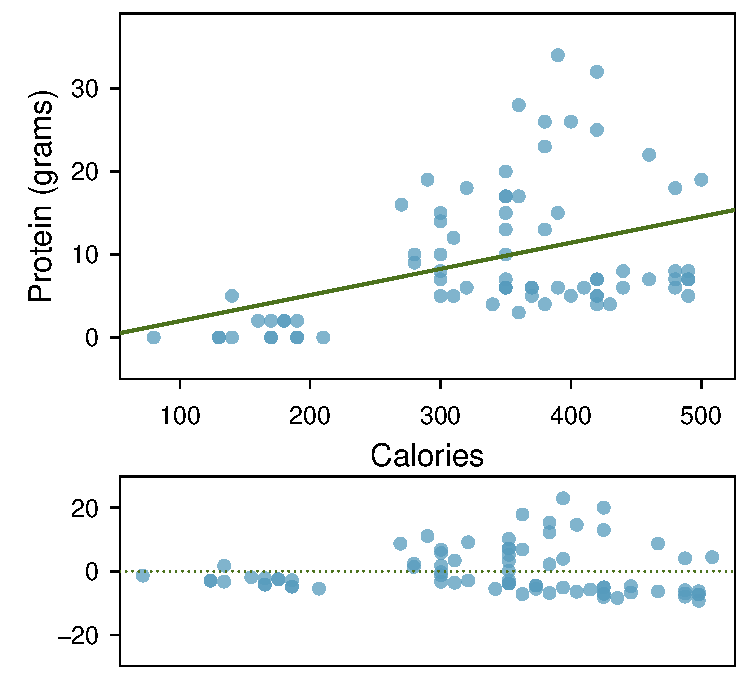
\includegraphics[width=0.38\textwidth]{ch_regr_simple_linear/figures/eoce/starbucks_cals_protein/starbucks_cals_protein}}
\end{center}
}{}

% 42 - helmet_lunch_ahss

\eoce{\qt{Helmets and lunches\label{helmet_lunch_ahss}}
The scatterplot shows the 
relationship between socioeconomic status measured as the percentage of 
children in a neighborhood receiving reduced-fee lunches at school 
({\tt lunch}) and the percentage of bike riders in the neighborhood 
wearing helmets ({\tt helmet}). The average percentage of children 
receiving reduced-fee lunches is 30.8\% with a standard deviation 
of 26.7\% and the average percentage of bike riders wearing helmets 
is 38.8\% with a standard deviation of 16.9\%.

\noindent\begin{minipage}[c]{0.5\textwidth}
{\raggedright\begin{parts}
\item If the $R^2$ for the least-squares regression line for these 
data is $72\%$, what is the correlation between {\tt lunch} 
and {\tt helmet}?
\item Calculate the slope and intercept for the least-squares regression 
line for these data.
\item Interpret the intercept of the least-squares regression line in 
the context of the application.
\item Interpret the slope of the least-squares regression line in the 
context of the application.
\item What would the value of the residual be for a neighborhood where 
40\% of the children receive reduced-fee lunches and 40\% of the bike 
riders wear helmets? Interpret the meaning of this residual in the context 
of the application.
\end{parts}}
\end{minipage}
\begin{minipage}[c]{0.05\textwidth}
$\:$ \\
\end{minipage}
\begin{minipage}[c]{0.42\textwidth}
\begin{center}
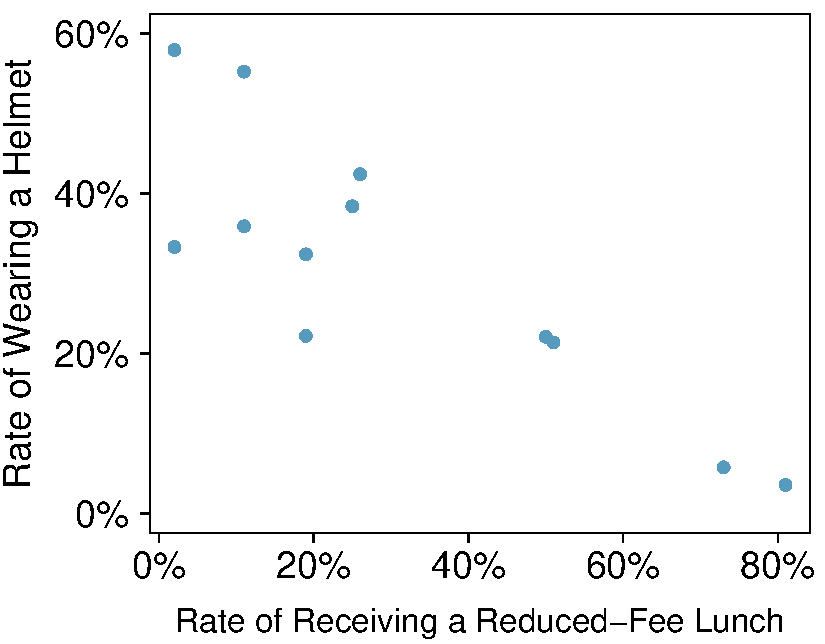
\includegraphics[width=\textwidth]{ch_regr_simple_linear/figures/eoce/helmet_lunch_ahss/helmet_lunch.pdf} \\
\end{center}
\end{minipage}
}{}

\D{\newpage}

% 43 - match_corr_3

\eoce{\qt{Match the correlation, Part III\label{match_corr_3}} 
Match each correlation to the corresponding scatterplot.

\noindent%
\begin{minipage}[c]{0.17\textwidth}
\begin{parts}
\item $r = -0.72$
\item $r = 0.07$ 
\item $r = 0.86$ 
\item $r = 0.99$
\end{parts}\vspace{3mm}
\end{minipage}%
\begin{minipage}[c]{0.83\textwidth}
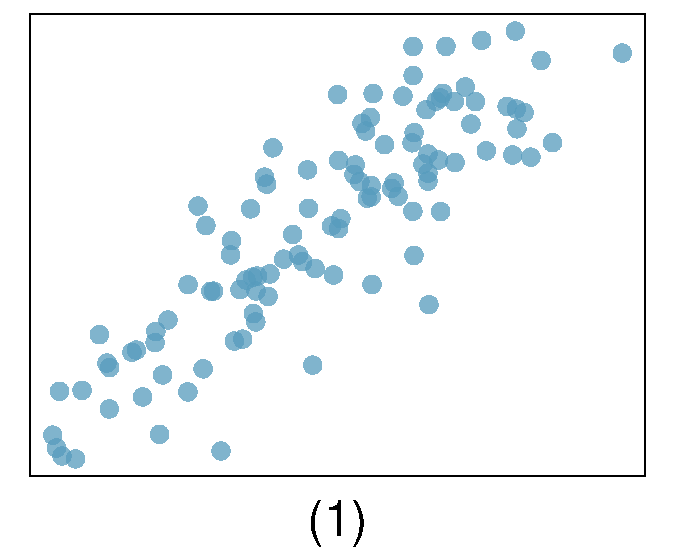
\includegraphics[width=0.245\textwidth]{ch_regr_simple_linear/figures/eoce/match_corr_3/scatter_1}
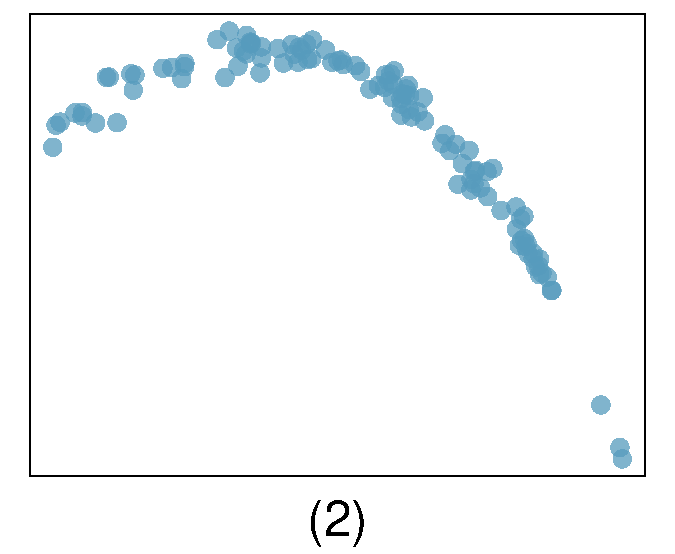
\includegraphics[width=0.245\textwidth]{ch_regr_simple_linear/figures/eoce/match_corr_3/scatter_2}
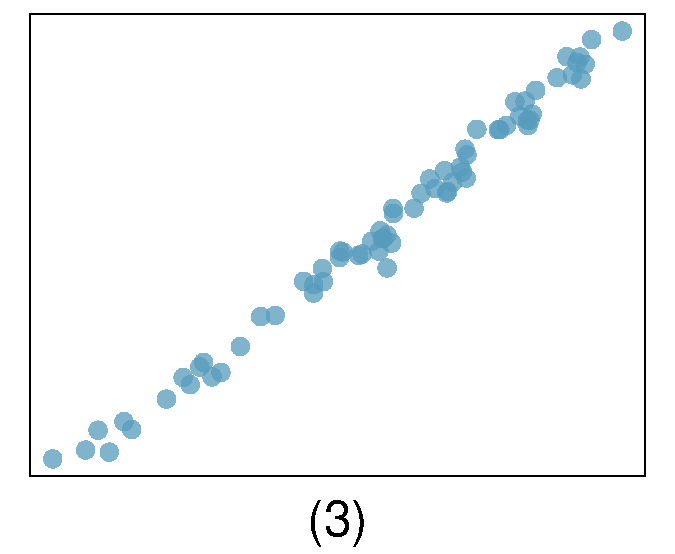
\includegraphics[width=0.245\textwidth]{ch_regr_simple_linear/figures/eoce/match_corr_3/scatter_3}
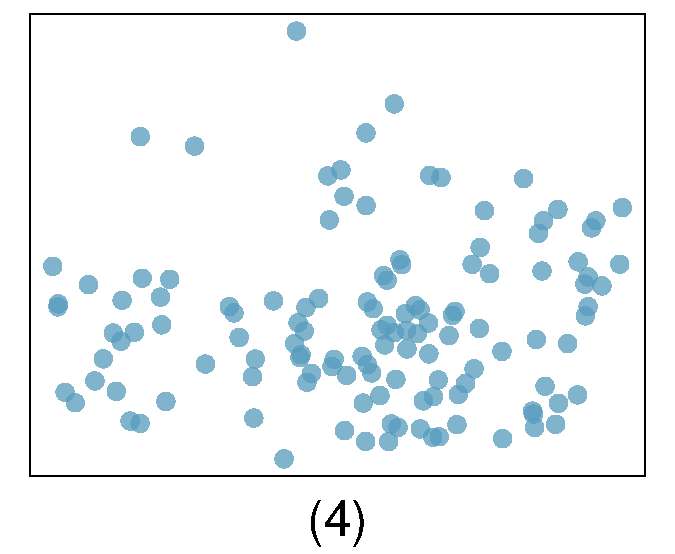
\includegraphics[width=0.245\textwidth]{ch_regr_simple_linear/figures/eoce/match_corr_3/scatter_4}
\end{minipage}
}{}

% 44 - rate_my_prof_ahss

\eoce{\qt{Rate my professor\label{rate_my_prof_ahss}}
Many college courses conclude by giving students
the opportunity to evaluate the course and the
instructor anonymously.
However, the use of these student evaluations
as an indicator of course quality and teaching
effectiveness is often criticized because these
measures may reflect the influence of
non-teaching related characteristics,
such as the physical appearance of the instructor.
Researchers at University of Texas, Austin
collected data on teaching evaluation score
(higher score means better) and standardized
beauty score (a score of 0 means average, negative
score means below average, and a positive score
means above average) for a sample of 463
professors.\footfullcite{Hamermesh:2005}
The scatterplot below shows the relationship
between these variables, and regression output
is provided for predicting teaching evaluation
score from beauty score.
\begin{center}
\begin{tabular}{rrrrr}
    \hline
            & Estimate  & Std. Error    & t value   & Pr($>$$|$t$|$) \\ 
  \hline
(Intercept) & 4.010     & 0.0255        & 	157.21  & 0.0000 \\ 
beauty      &  \fbox{\textcolor{white}{{\footnotesize Cell 1}}}  
                        & 0.0322        & 4.13      & 0.0000\vspace{0.8mm} \\ 
   \hline
\end{tabular}
\end{center}
\noindent\begin{minipage}[c]{0.45\textwidth}
{\raggedright\begin{parts}
\item
    Given that the average standardized beauty score
    is -0.0883 and average teaching evaluation score
    is 3.9983, calculate the slope.
    Alternatively, the slope may be computed using just
    the information provided in the model summary table.
\item
    Do these data provide convincing evidence that the
    slope of the relationship between teaching evaluation
    and beauty is positive?
    Explain your reasoning.
\item
    List the conditions required for linear regression
    and check if each one is satisfied for this model
    based on the following diagnostic plots.
\end{parts}}
\end{minipage}
\begin{minipage}[c]{0.07\textwidth}
$\:$ \\
\end{minipage}
\begin{minipage}[c]{0.45\textwidth}
\tabspecial{tableau-teaching-eval-beauty}{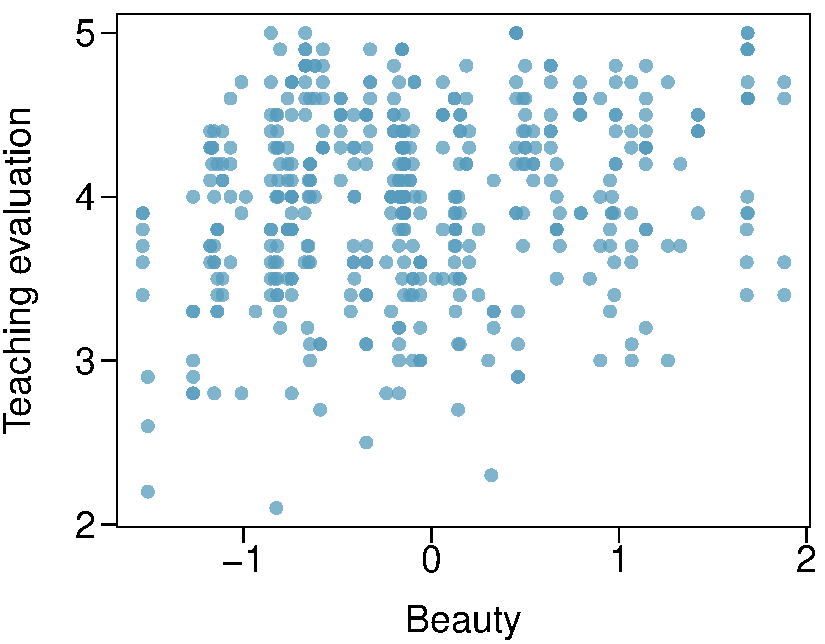
\includegraphics[width=\textwidth]{ch_regr_simple_linear/figures/eoce/rate_my_prof_ahss/rate_my_prof_eval_beauty.pdf}} \\
\end{minipage}
\begin{center}
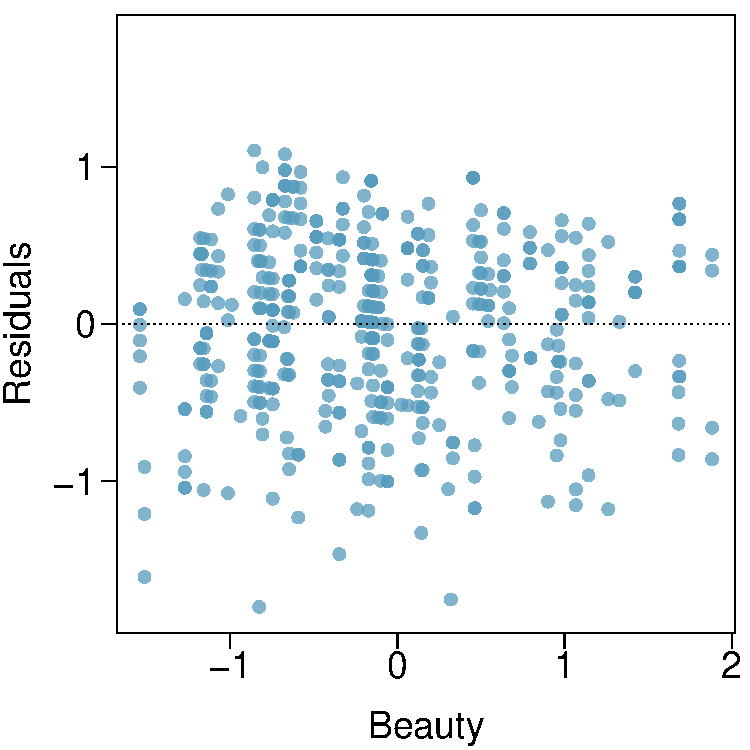
\includegraphics[width=0.32\textwidth]{ch_regr_simple_linear/figures/eoce/rate_my_prof_ahss/rate_my_prof_residuals}
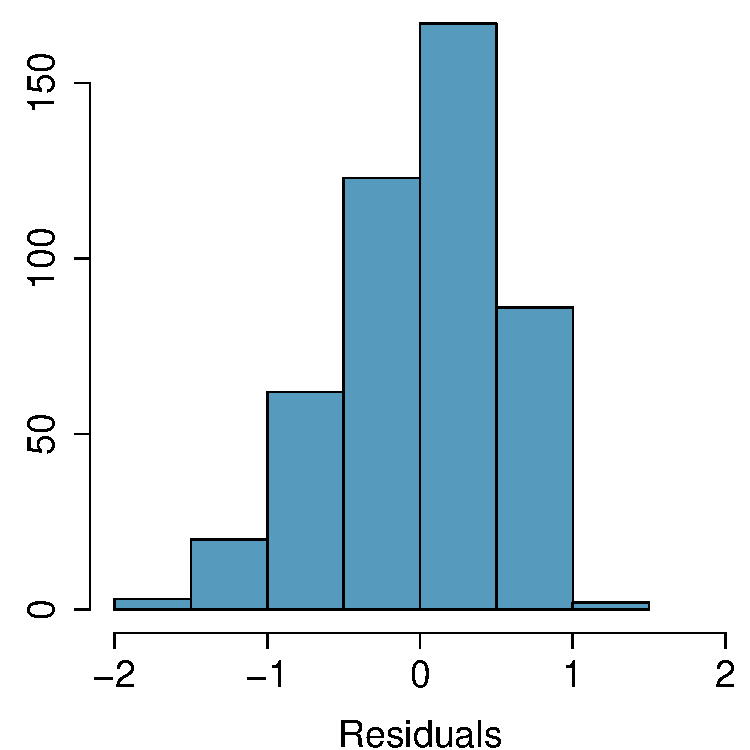
\includegraphics[width=0.32\textwidth]{ch_regr_simple_linear/figures/eoce/rate_my_prof_ahss/rate_my_prof_residuals_hist}
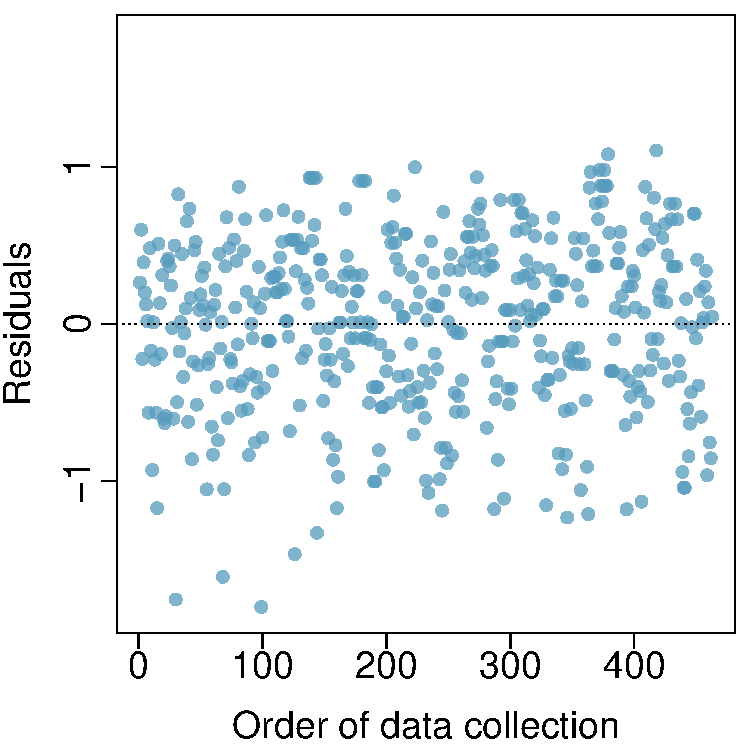
\includegraphics[width=0.32\textwidth]{ch_regr_simple_linear/figures/eoce/rate_my_prof_ahss/rate_my_prof_residuals_order}
\end{center}
}{}

\D{\newpage}

% 45 - trees_volume_height_diameter

\eoce{\qt{Trees\label{trees_volume_height_diameter}} The scatterplots below 
show the relationship between height, diameter, and volume of timber 
in 31 felled black cherry trees. The diameter of the tree is measured 
4.5 feet above the ground.\footfullcite{data:trees}
\begin{center}
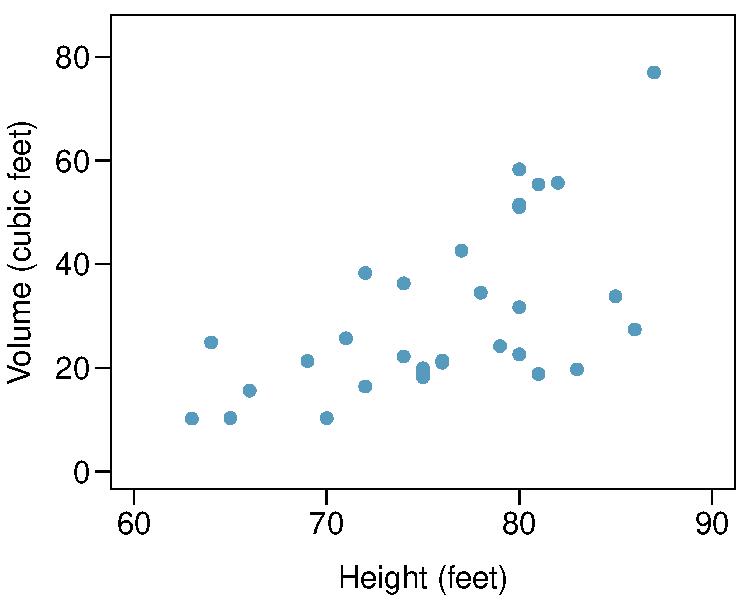
\includegraphics[width=0.46\textwidth]{ch_regr_simple_linear/figures/eoce/trees_volume_height_diameter/trees_volume_height.pdf}
\hspace{0.07\textwidth}%
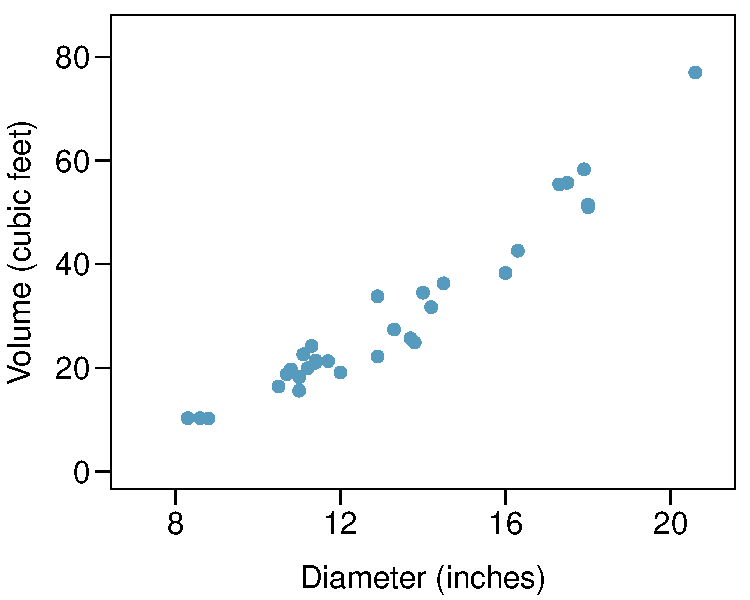
\includegraphics[width=0.46\textwidth]{ch_regr_simple_linear/figures/eoce/trees_volume_height_diameter/trees_volume_diameter.pdf}
\end{center}
\begin{parts}
\item Describe the relationship between volume and height of these trees.
\item Describe the relationship between volume and diameter of these trees.
\item Suppose you have height and diameter measurements for another black 
cherry tree. Which of these variables would be preferable to use to predict 
the volume of timber in this tree using a simple linear regression model? 
Explain your reasoning.
\end{parts}
}{}

  }



%-------------------------------------------------------------
% 5 Section Headers
%
% See headers.tex file for main chapters.
\newcommand{\chapterpagepaddingtopinner}[0]{35mm} % 45mm
\newcommand{\chapterpagepaddingrightinner}[0]{30mm}
\newcommand{\chapterpagepaddinginner}[0]{25mm}
\newcommand{\chapterXfontsize}[0]{92}
\newcommand{\chaptertitlefontsize}[0]{30}


%-------------------------------------------------------------
% 6 Utilities
% 6.1 Helpful Editing Commands
\newcommand\Add[1]{\marginpar[{\Huge\color{oiR}$\bullet$}]{\Huge\color{oiR}$\bullet$}{\color{oiB}#1}}
\newcommand\Cut[1]{\marginpar[{\Huge\color{oiR}$\bullet$}]{\Huge\color{oiR}$\bullet$}{\color{oiGC}#1}}
\newcommand\Comment[1]{\marginpar[{\Huge\color{oiR}$\bullet$}]{\Huge\color{oiR}$\bullet$} {\color{oiG}{[#1]}}}
\newcommand{\note}[1]{\Comment{#1}}
% 6.2 Special Symbols
\newcommand{\degree}{\ensuremath{^\circ}}
\newcommand{\R}{\textbf{\textsf{R}}}
% 6.3 Text Commands (Terms, Data, Variable, Response)
\newcommand{\term}[1]{\textbf{#1}\index{#1|textbf}}
\newcommand{\termsub}[2]{\textbf{#1}\index{#2|textbf}}
\newcommand{\termni}[1]{\textbf{#1}}
\newcommand{\hiddenterm}[1]{#1\index{#1|textbf}}
\newcommand{\indexthis}[2]{#1\index{#2}}
\newcommand{\termO}[1]{\textbf{\color{termOColor}#1}}
\newenvironment{data}[1]{\texttt{#1}}{}
\newcommand{\datalink}[1]{\index{#1|textbf}\texttt{\oiRedirect{data_#1}{#1}}}
\newenvironment{var}[1]{\texttt{#1}}{}
\newenvironment{resp}[1]{\texttt{#1}}{}
\newcommand{\lmlevel}[1]{:~\emph{#1}}{}
\newenvironment{calctext}[1]{{\color{oiB}\texttt{#1}}}{}
\newenvironment{calctextmath}[1]{{\color{oiB}\mathtt{#1}}}{}
\newenvironment{calcbutton}[1]{{\color{oiB}\texttt{#1}}}{}
\newcommand{\codeindent}{\hspace{5mm}}
% 6.4 Highlighting
\newenvironment{highlight}{\textbf}{}
\newcommand{\highlightO}[1]{\textbf{\color{oiB}#1}}
\newcommand{\highlightT}[1]{\emph{\color{oiR}#1}}
% 6.5 Lengths
\setlength{\parindent}{0.3in}
% 6.6 Hyperreferences
\newcommand{\urlwofont}[1]{\urlstyle{same}\url{#1}}
%\newcommand{\oiRedirect}[2]{\href{http://www.openintro.org/redirect.php?go=#1&referrer=\referrer}{#2}}
\newcommand{\oiRedirectUrl}[1]{http://www.openintro.org/redirect.php?go=#1&referrer=ahss2_pdf}
\newcommand{\oiRedirect}[2]{\href{\oiRedirectUrl{#1}}{#2}}
\newcommand{\videoicon}[1][4.5mm]{
\includegraphics[height=#1]{extraTeX/icons/video_camera.png}~}
\newcommand{\CalculatorVideos}[1]{}%{\begin{tipBox}{\tipBoxTitle[\videoicon]{Calculator videos}
%Videos covering #1 using TI and Casio graphing calculators are available at \mbox{\oiRedirect{textbook-openintro_videos}{openintro.org/videos}}.}
%\end{tipBox}}
\newcommand{\videohref}[2][4.5mm]{\oiRedirect{#2}{\raisebox{-0.3mm}[0pt]{
\includegraphics[height=#1]{extraTeX/icons/video_camera.png}}}}
\newcommand{\tableauhref}[2][4.5mm]{\oiRedirect{#2}{\raisebox{-0.3mm}[0pt]{
\includegraphics[height=#1]{extraTeX/icons/tableau}}}}
\newcommand{\slideshref}[2][4.5mm]{\oiRedirect{#2}{\raisebox{-0.3mm}[0pt]{
\includegraphics[height=#1]{extraTeX/icons/slides.png}}}}
\newcommand{\videomarginhref}[2][4mm]{\oiRedirect{#2}{\raisebox{-3mm}[0pt]{
\includegraphics[height=#1]{extraTeX/icons/video_camera.png}}}}
\newcommand{\sectionvideohref}[2][6mm]{\oiRedirect{#2}{\raisebox{-0.5mm}[0pt]{
\includegraphics[height=#1]{extraTeX/icons/video_camera.png}}}}
\newcommand{\sectionslideshref}[2][6mm]{\oiRedirect{#2}{\raisebox{-0.5mm}[0pt]{
\includegraphics[height=#1]{extraTeX/icons/slides.png}}}}
\newcommand{\MarginVideo}[1]{\marginpar[{\videomarginhref{#1}}]{{\videomarginhref{#1}}}}
% 6.7 Helper commands
\newcommand{\us}[0]{\_\hspace{0.3mm}}
%\newcommand{\quadplus}[0]{\quad + \quad}
\newcommand{\indfunc}[2]{\var{#1}_{\resp{#2}}}


%-------------------------------------------------------------
% 7 Inference steps

\newcommand{\inferencestep}[1]{\textbf{#1}:}


%-------------------------------------------------------------
% 8 Figures and Captions
% 8.1 & 8.2 Table & Figure Numbering
% Thanks @Herbert on StackExchange for helping clean up this style code!
% http://tex.stackexchange.com/questions/176978/latex-numbering-in-counters-appears-to-have-changed/177045?noredirect=1#comment409945_177045
\makeatletter
\let\c@table\c@figure
\makeatother
% 8.3 Caption Width
\newlength{\mycaptionwidth}
\setlength{\mycaptionwidth}{0.825\textwidth}
\setlength{\captionwidth}{\mycaptionwidth}
\newcommand{\Figure}[2]{\includegraphics[width=#1\textwidth]{\chapterfolder/figures/#2/#2}}
\newcommand{\Figures}[3]{\includegraphics[width=#1\textwidth]{\chapterfolder/figures/#2/#3}}
\newcommand{\Figuress}[3]{\includegraphics[width=#1]{\chapterfolder/figures/#2/#3}}
\newcommand{\chapterfolder}{}




%-------------------------------------------------------------
% 9 Examples and Exercises
% 9.1 Exercises, within the text
% 9.1.1 Exercise Environment
\newcommand{\excolor}[1]{{\color{excolor}#1}}
\newenvironment{exercise}
{
\begin{itemize}\item[\color{oiB}$\bigodot$]\refstepcounter{equation}\noindent\normalsize\textbf{\color{oiB}Guided Practice \theexercise}%\hspace{3mm}

}
{\normalsize

\stdaddvspace{}
\end{itemize}}
% 9.1.2 Exercise Fine Tuning
\newcommand\theexercise{\thechapter.\arabic{equation}}
% 9.2 Examples
% 9.2.1 Example Environment
\newcommand\theexample{\thechapter.\arabic{equation}}
\newenvironment{example}[1]
{\begin{itemize}
\item[\color{oiB}\Large$\CIRCLE$]\refstepcounter{equation}\noindent\textbf{\color{oiB}Example \theexample}

#1\vspace{\exampleAboveBar}

{\color{examplegray}\rule{20mm}{0.1mm}}

\vspace{\exampleBelowBar}

\normalsize}{

\end{itemize}
\stdaddvspace{}
}
% 9.2.2 Wrappers
%\reversemarginpar
\def\warningsymbol{\protect\marginsymbolhelper}
\def\marginsymbolhelper{\tabto*{0mm} {\dbend} \tabto*{0mm}}
\newcommand{\exampleicon}[1]{\vspace{#1} \raggedleft
\includegraphics[width=5mm]{extraTeX/icons/example.png}\hspace{2mm}\ }
\newenvironment{gpewrapper}[1]{\addvspace{4mm}

\noindent\hspace{-12.45mm}\begin{minipage}[c]{\textwidth+8mm}
\begin{minipage}[c]{8.4mm}
\hspace{0.5mm}\includegraphics[width=5mm]{extraTeX/icons/#1.png}
\end{minipage}\begin{minipage}[c]{\textwidth-0.45mm}\begin{mdframed}[%
    topline=false,
    rightline=false,
    bottomline=false,
    linewidth=0.5mm,
    linecolor=oiB]}{\end{mdframed}\end{minipage}\end{minipage}

    \addvspace{4mm}}
\newenvironment{examplewrap}
    {\begin{gpewrapper}{example}}
    {\end{gpewrapper}}
\newenvironment{exercisewrap}
    {\begin{gpewrapper}{guided_practice}}
    {\end{gpewrapper}}
% 9.2.3 Example Title
\newcommand{\exampletitle}[1]{\textbf{\color{oiB}\small\fontfamily{phv}%
\selectfont{\MakeUppercase{Example~#1}}} \\[1mm]}
\newcommand{\exercisetitle}[1]{\textbf{\color{oiB}\small\fontfamily{phv}%
\selectfont{\MakeUppercase{Guided Practice~#1}}} \\[1mm]}
% 9.2.4 NEW Example and Guided Practice Environment
\newcommand{\exspace}{\stdvspace{}}
\newenvironment{nexample}[1]{\addvspace{6mm}

\refstepcounter{equation}\exampletitle{\theexample}
#1

\addvspace{\nexampleAboveBar}

{\color{examplegray}\rule{20mm}{0.1mm}}

\addvspace{\nexampleBelowBar}

\setlength{\parskip}{2mm}}{}
\newenvironment{nexercise}{\addvspace{6mm}

\refstepcounter{equation}\exercisetitle{\theexample}}{}

% 9.3 EOCEs: End of Chapter Exercises
% 9.3.1 Environment
\newenvironment{eoce}[2][]
{\refstepcounter{eoce}\noindent\small\textbf{\textcolor{oiB}{{\hypersetup{linkcolor=oiB}{\fontfamily{phv}\selectfont\ref{eoce_sol_\arabic{chapter}_\arabic{eoce}}}}\label{eoce_\arabic{chapter}_\arabic{eoce}}}}\hspace{2mm} #1#2

\addvspace{4mm}

}
%{\em #2 } $\:$ \\ }
{}
% 9.3.2 EOCE Solutions
\newcommand{\eocesolch}[1]{
\refstepcounter{eocesolch}\noindent\textbf{\color{oiB}\arabic{eocesolch}\hspace{2mm}#1}

\addvspace{2mm}

}
{
\newcommand{\eocesol}[1]{\refstepcounter{eocesol}\noindent\textbf{\color{oiB}{\hypersetup{linkcolor=oiB}{\fontfamily{phv}\selectfont\ref{eoce_\arabic{eocesolch}_\arabic{eocesol}}}}\label{eoce_sol_\arabic{eocesolch}_\arabic{eocesol}}}\hspace{2mm}{\small#1}\makebox[0pt]{\color{white}\tiny \refstepcounter{eocesol}\label{eoce_sol_\arabic{eocesolch}_\arabic{eocesol}}}

\addvspace{1mm}

}
% 9.3.3 EOCE Utilities
\newcommand{\qt}[2][.]{{\fontfamily{phv}\selectfont\textcolor{oiB}{\textbf{#2#1}}}}
\newcommand{\qtq}[1]{{\fontfamily{phv}\selectfont\textcolor{oiB}{\textbf{#1?}}}}
\newcommand{\ec}[1]{\textcolor{oiB}{\footnotesize{~(#1)}}}% 9.3.4 EOCE Roman Parts
\newenvironment{romanparts}{
\begin{enumerate}[I.]
\setlength{\itemsep}{0mm}
}{\end{enumerate}}
% 9.3.5 EOCE Parts
\newenvironment{parts}{
%\vspace{-0.25cm}
\begin{enumerate}[(a)]
\setlength{\itemsep}{0mm}}
{\end{enumerate}}
% 9.3.6 EOCE Subparts
\newenvironment{subparts}{
\begin{enumerate}[i.]
\setlength{\itemsep}{0mm}}
{\end{enumerate}}
% 9.3.7 EOCE hyp environment
\newenvironment{hyp}{
\begin{itemize}
\setlength{\itemsep}{0mm}
}
{\end{itemize}
}
% 9.3.8 cond environment
\newenvironment{cond}{
\begin{enumerate}[1.]
\setlength{\itemsep}{0mm}
}
{\end{enumerate}
}
% 9.3.9 Exercise fixes required.
\newcommand{\eoceNeedSolution}[1][]
{\textbf{\refstepcounter{eoceNeedSolution} \color{red}ADD SOLUTION. #1}}
\newcommand{\eoceReplace}[1][]
{\textbf{\refstepcounter{eoceReplace} \color{red}REPLACE THIS EXERCISE. #1}}
\newcommand{\eoceFF}[1][]
{\textbf{\refstepcounter{eoceFF} \color{red}FINAL FORMATTING.}}





%-------------------------------------------------------------
% 10 Special Boxes
% 10.1.1 Term Box
\newcommand\tBoxTitleBuffer{\\[1.5mm]}
\newenvironment{tBoxTitle}[2][\tBoxTitleBuffer]{\textbf{\color{oiB}#2} #1
}{}
\newenvironment{termBox}[1]{
\addvspace{4mm}
\noindent{\color{oiB}\framebox[\textwidth][c]{\framebox[\textwidth-3mm][l]{ \\
	\vspace{0.5cm} \\
	\begin{minipage}[b]{\textwidth-3mm}
		\begin{minipage}[t]{2mm}
			\hspace{2mm}
		\end{minipage}
		\begin{minipage}[b]{\textwidth-10mm}
			\color{black}\ \\[-0.7mm]
			#1
			
			\vspace{1mm}
		\end{minipage}
	\end{minipage}}}}
}{

\addvspace{1mm}}
% 10.2 Tip Box
\newenvironment{tipBoxTitle}[2][TIP:\ ]{\textbf{\color{oiB}#1#2}\\[0.3mm]}{}
\newenvironment{tipBox}[1]{
\addvspace{4mm}
\noindent{\color{oiB}\framebox[\textwidth][l]{ \\
	\vspace{5mm} \\
	\begin{minipage}[b]{\textwidth-4mm}
		\begin{minipage}[t]{2mm}
			\hspace{2mm}
		\end{minipage}
		\begin{minipage}[b]{\textwidth-8mm}
			\color{black}\ \\[-0.7mm]
			#1
			
			\vspace{1mm}
		\end{minipage}
	\end{minipage}}}
}{

\addvspace{1mm}}
% 10.3 Caution Box
\newenvironment{caution}[2]{
\addvspace{4mm}
\noindent{\color{oiB}\framebox[\textwidth][l]{ \\
	\vspace{5mm} \\
	\begin{minipage}[b]{\textwidth-4mm}
		\begin{minipage}[t]{2mm}
			\hspace{2mm}
		\end{minipage}
		\begin{minipage}[b]{\textwidth-8mm}
			\textbf{\color{oiB}Caution: #1} \\[1mm]
			\color{black}#2
		\end{minipage}
	\end{minipage}}}
}{

\addvspace{1mm}}
% 10.4 One Box
\newenvironment{onebox}[1]{
\addvspace{4mm}
\noindent\begin{minipage}{\textwidth}
\noindent\rule{\textwidth}{0.3pt}\vspace{-6mm}
\begin{mdframed}[%
    topline=false,
    rightline=false,
    leftline=false,
    bottomline=false,
    backgroundcolor=grayBackground]
\textbf{\color{oiB}\small\fontfamily{phv}%
\selectfont{\MakeUppercase{#1}}} \\[1mm]}{
\end{mdframed}\vspace{-4.2mm}
\rule{\textwidth}{0.3pt}
\end{minipage}

\addvspace{4mm}}

%% exercise tags
\newcommand{\tabspecial}[1]{\oiRedirect{#1}{\tableauhref{#1}}}

\newcommand{\videosolution}[1]{\videohref{#1}\ \ }






%% 1 Page Parameters
% 2 Special Commands for Editions
% 3 Content Modifications
% 4 Counters and Parameters
% 5 Section Coloring
% 6 Utilities
% 7 
% 8 Figures and Captions
% 9 Examples and Exercises
% 10 Special Boxes

%\renewcommand\chapter{\if@openright\cleardoublepage\else\clearpage\fi
%                    \thispagestyle{fancy}%
%                    \global\@topnum\z@
%                    \@afterindentfalse
%                    \secdef\@chapter\@schapter}
\fancypagestyle{plain}{%
\fancyhf{} % clear all header and footer fields
\fancyhead[RO,RE]{\thepage} %RO=right odd, RE=right even
\renewcommand{\headrulewidth}{0pt}
\renewcommand{\footrulewidth}{0pt}}
\raggedbottom


\newcommand{\stdspace}[0]{3mm}
\newcommand{\stdvspace}[0]{\vspace{\stdspace{}}}
\newcommand{\stdaddvspace}[0]{\addvspace{\stdspace{}}}




%-------------------------------------------------------------
% 1 Page Parameters
% 1.1
\setlength\paperheight{11in}
\setlength\paperwidth{8.5in}
\newcommand{\officialtextheight}{9.7in}
\newcommand{\officialtextwidth}{6in}
%\setlength\paperheight{10in}
%\setlength\paperwidth{8in}
%\newcommand{\officialtextheight}{8.7in}
%\newcommand{\officialtextwidth}{6in}
\newcommand{\officialvoffset}{-0.6in}
\setlength\textheight{\officialtextheight}
\setlength\textwidth{\officialtextwidth}
\setlength\voffset{\officialvoffset}
\renewcommand{\baselinestretch}{1.0}
% 1.2 Margin Size
% 1.2.1 Slim
%\setlength\hoffset{0.25in}
%\setlength\oddsidemargin{0.25in}
%\setlength\evensidemargin{0in}
% 1.2.2 Medium
\setlength\hoffset{3.7mm}
\setlength\oddsidemargin{3mm}
\setlength\evensidemargin{3mm}
% 1.2.3 Wide
%\setlength\hoffset{-5mm}
%\setlength\oddsidemargin{0.5in}
%\setlength\evensidemargin{0.5in}
% 1.3 PDF Parameters
%\setlength\paperheight{11in}
%\setlength\textheight{8.25in}
%\setlength\paperwidth{8.5in}
%\setlength\textwidth{5.45in}
%\setlength\voffset{-10mm}
%\setlength\oddsidemargin{0.75in}
%\setlength\evensidemargin{0.75in}
% 1.4 Margin Spacing
\setlength{\marginparsep}{5mm}
\setlength{\marginparwidth}{20mm}
% 1.5 Page Header
\pagestyle{fancy}
\renewcommand{\headrulewidth}{0pt}
\fancyhead[RO,LE]{\thepage}
\fancyhead[RE]{\leftmark}
\fancyhead[LO]{\rightmark}
\fancyfoot[c]{}
\fancyheadoffset[RO,LE]{0.9in}



% Tablet Version
%\setlength\paperheight{8.82in}\setlength\textheight{8.25in}\setlength\paperwidth{5.7in}\setlength\textwidth{5.45in}\setlength\voffset{-23.5mm}\setlength\hoffset{-27mm}\setlength\oddsidemargin{5mm}\setlength\evensidemargin{5mm}\setlength{\marginparsep}{5mm}\setlength{\marginparwidth}{35mm}\fancyheadoffset[RO,LE]{0.2in}




%-------------------------------------------------------------
% 2 Special Commands for Editions
\newcommand{\referrer}{AHSS3_pdf}
\newcommand{\vspaceB}[1]{}
\newcommand{\hspaceB}[1]{}
\newcommand{\textB}[1]{}
\newcommand{\textC}[1]{}
\newcommand{\B}[1]{#1}

\newcommand{\D}[1]{#1}



%-------------------------------------------------------------
% 3 Content Modifications
\newcommand{\APVersion}[2]{#2}
\newcommand{\MultipleRegression}[2]{#1}
\newcommand{\MultipleRegressionChapter}[2]{#1}
\newcommand{\SimulationAndRandomization}[1]{#1}
\newcommand{\ANOVASection}[2]{#1}
\newcommand{\GLMSection}[2]{#1}




%-------------------------------------------------------------
% 4 Counters and Parameters
% 4.1 Counters
\newcounter{alwaysOne}
\setcounter{alwaysOne}{1}
\newcounter{alwaysTwo}
\setcounter{alwaysTwo}{2}
\newcounter{alwaysThree}
\setcounter{alwaysThree}{3}
\newcounter{alwaysFour}
\setcounter{alwaysFour}{4}
\newcounter{withinChNum}[chapter]
\setcounter{withinChNum}{0}
\newcounter{eoce}[chapter]
\renewcommand{\theeoce}
    {\arabic{chapter}.\arabic{eoce}}
\newcounter{eocesolch}
\setcounter{eocesolch}{0}
\newcounter{eocesol}[eocesolch]
\renewcommand{\theeocesol}
     {\arabic{eocesolch}.\arabic{eocesol}}
\newcounter{eoceNeedSolution}[chapter]
\renewcommand{\theeoceNeedSolution}
    {\arabic{chapter}.\arabic{eoceNeedSolution}}
\newcounter{eoceReplace}[chapter]
\renewcommand{\theeoceReplace}
    {\arabic{chapter}.\arabic{eoceReplace}}
\newcounter{eoceFF}[chapter]
\renewcommand{\theeoceFF}
    {\arabic{chapter}.\arabic{eoceFF}}
% 4.2 Parameters
\newlength{\exampleAboveBar}
\newlength{\exampleBelowBar}
\setlength{\exampleAboveBar}{-3.15mm}
\setlength{\exampleBelowBar}{-1.15mm}
\newlength{\nexampleAboveBar}
\newlength{\nexampleBelowBar}
\setlength{\nexampleAboveBar}{-1mm}
\setlength{\nexampleBelowBar}{-1mm}
% 4.3 Chapter Declarations
\newcommand\includechapter[2]{
  \setcounter{chapter}{#1}
  \addtocounter{chapter}{-1}
  \normalsize
  \include{#2/TeX/#2}
  \newpage\reviewexercisesheader{}

% 39 - tf_correlation

\eoce{\qt{True / False\label{tf_correlation}}
Determine if the following statements are true or false.
If false, explain why.
\begin{parts}
\item A correlation coefficient of -0.90 indicates a stronger 
linear relationship than a correlation of 0.5.
\item Correlation is a measure of the association between any 
two variables.
\end{parts}
}{}

% 40 - cat_body_heart_inf_2s_ahss

\eoce{\qt{Cats, Part II\label{cat_body_heart_inf_ahss}}
Exercise~\ref{cat_body_heart_reg} 
presents regression output from a model for predicting the heart 
weight (in g) of cats from their body weight (in kg). The coefficients 
are estimated using a dataset of 144 domestic cat. The model output 
is also provided below.  Assume that conditions for inference on the slope are met.
\begin{center}
\begin{tabular}{rrrrr}
    \hline
            & Estimate  & Std. Error    & t value   & Pr($>$$|$t$|$) \\ 
    \hline
(Intercept) & -0.357    & 0.692         & -0.515    & 0.607 \\ 
body wt     & 4.034     & 0.250         & 16.119    & 0.000 \\ 
    \hline
\end{tabular}
\[ s = 1.452 \qquad R^2 = 64.66\% \qquad R^2_{adj} = 64.41\% \]
\end{center}
\begin{parts}
\item 
    What are the hypotheses for evaluating whether body weight is
 associated with heart weight in cats?
\item State the conclusion of the hypothesis test from part (a) in 
context of the data.
\item Calculate a 95\% confidence interval for the slope of body 
weight, and interpret it in context of the data.
\item Do your results from the hypothesis test and the confidence 
interval agree? Explain.
\end{parts}
}{}

% 41 - starbucks_cals_protein

\eoce{\qt{Nutrition at Starbucks, Part II\label{starbucks_cals_protein}} 
Exercise~\ref{starbucks_cals_carbos} introduced a data set on nutrition 
information on Starbucks food menu items. Based on the scatterplot 
and the residual plot provided, describe the relationship between the 
protein content and calories of these menu items, and determine if a 
simple linear model is appropriate to predict amount of protein from 
the number of calories.
\begin{center}
\tabspecial{tableau-starbucks-p2}{
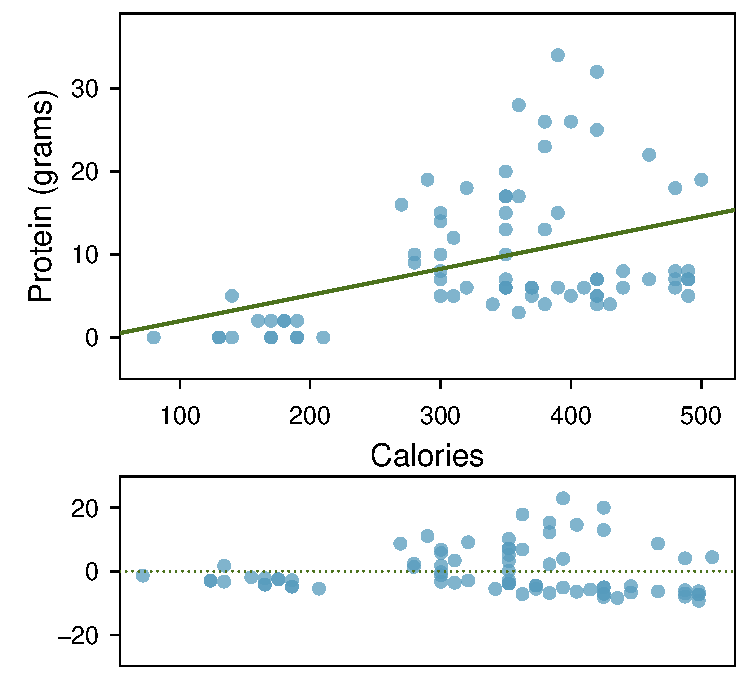
\includegraphics[width=0.38\textwidth]{ch_regr_simple_linear/figures/eoce/starbucks_cals_protein/starbucks_cals_protein}}
\end{center}
}{}

% 42 - helmet_lunch_ahss

\eoce{\qt{Helmets and lunches\label{helmet_lunch_ahss}}
The scatterplot shows the 
relationship between socioeconomic status measured as the percentage of 
children in a neighborhood receiving reduced-fee lunches at school 
({\tt lunch}) and the percentage of bike riders in the neighborhood 
wearing helmets ({\tt helmet}). The average percentage of children 
receiving reduced-fee lunches is 30.8\% with a standard deviation 
of 26.7\% and the average percentage of bike riders wearing helmets 
is 38.8\% with a standard deviation of 16.9\%.

\noindent\begin{minipage}[c]{0.5\textwidth}
{\raggedright\begin{parts}
\item If the $R^2$ for the least-squares regression line for these 
data is $72\%$, what is the correlation between {\tt lunch} 
and {\tt helmet}?
\item Calculate the slope and intercept for the least-squares regression 
line for these data.
\item Interpret the intercept of the least-squares regression line in 
the context of the application.
\item Interpret the slope of the least-squares regression line in the 
context of the application.
\item What would the value of the residual be for a neighborhood where 
40\% of the children receive reduced-fee lunches and 40\% of the bike 
riders wear helmets? Interpret the meaning of this residual in the context 
of the application.
\end{parts}}
\end{minipage}
\begin{minipage}[c]{0.05\textwidth}
$\:$ \\
\end{minipage}
\begin{minipage}[c]{0.42\textwidth}
\begin{center}
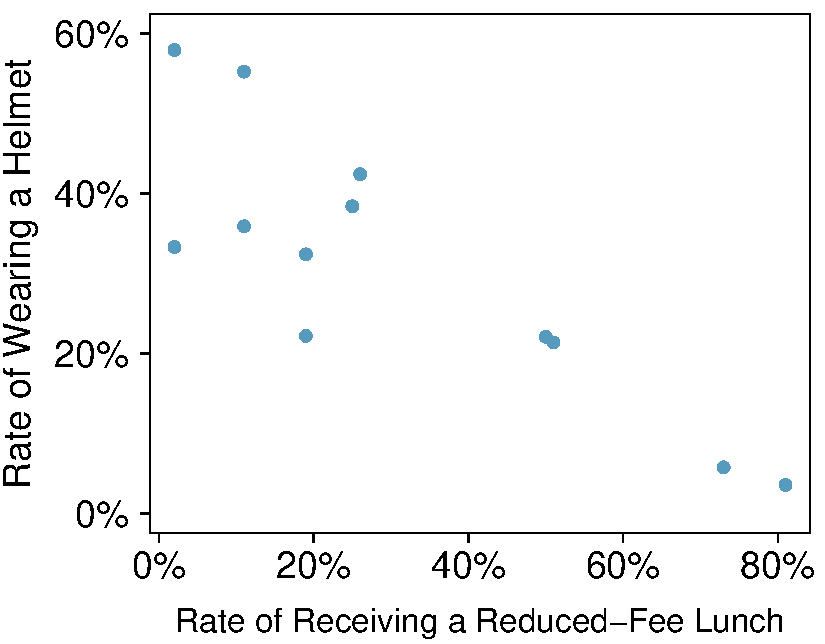
\includegraphics[width=\textwidth]{ch_regr_simple_linear/figures/eoce/helmet_lunch_ahss/helmet_lunch.pdf} \\
\end{center}
\end{minipage}
}{}

\D{\newpage}

% 43 - match_corr_3

\eoce{\qt{Match the correlation, Part III\label{match_corr_3}} 
Match each correlation to the corresponding scatterplot.

\noindent%
\begin{minipage}[c]{0.17\textwidth}
\begin{parts}
\item $r = -0.72$
\item $r = 0.07$ 
\item $r = 0.86$ 
\item $r = 0.99$
\end{parts}\vspace{3mm}
\end{minipage}%
\begin{minipage}[c]{0.83\textwidth}
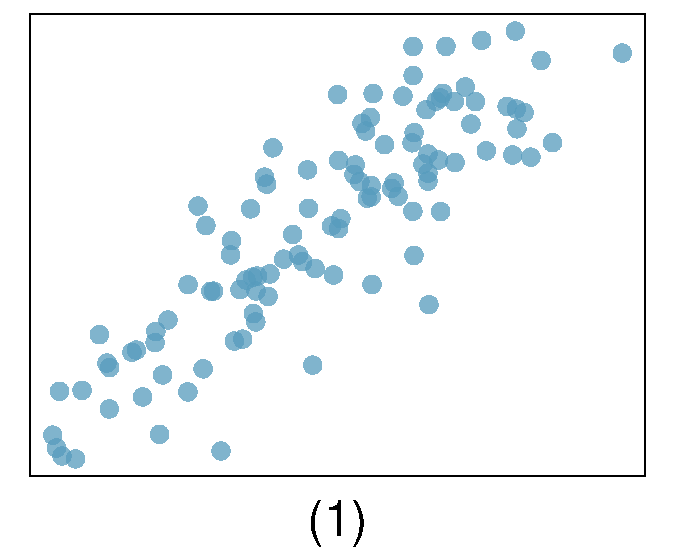
\includegraphics[width=0.245\textwidth]{ch_regr_simple_linear/figures/eoce/match_corr_3/scatter_1}
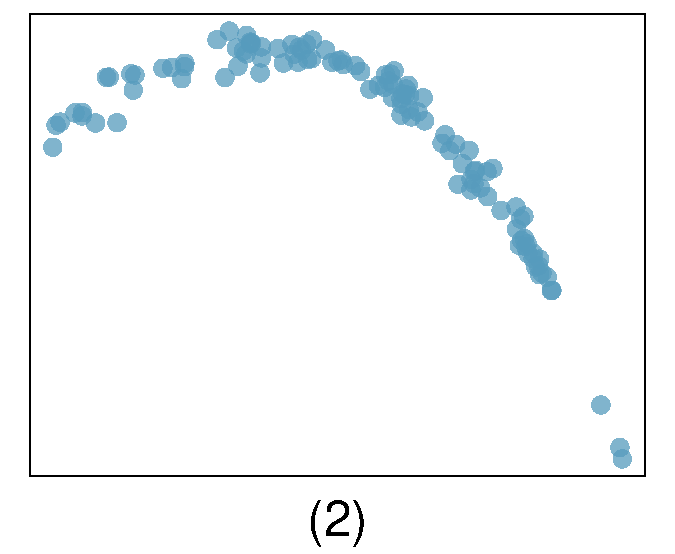
\includegraphics[width=0.245\textwidth]{ch_regr_simple_linear/figures/eoce/match_corr_3/scatter_2}
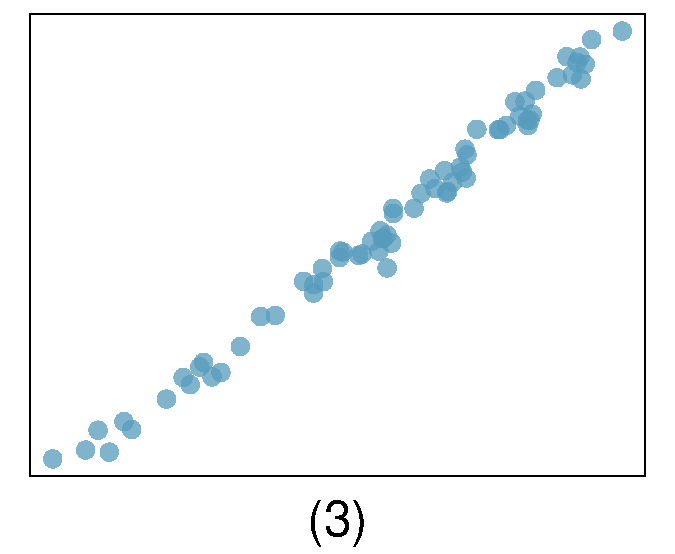
\includegraphics[width=0.245\textwidth]{ch_regr_simple_linear/figures/eoce/match_corr_3/scatter_3}
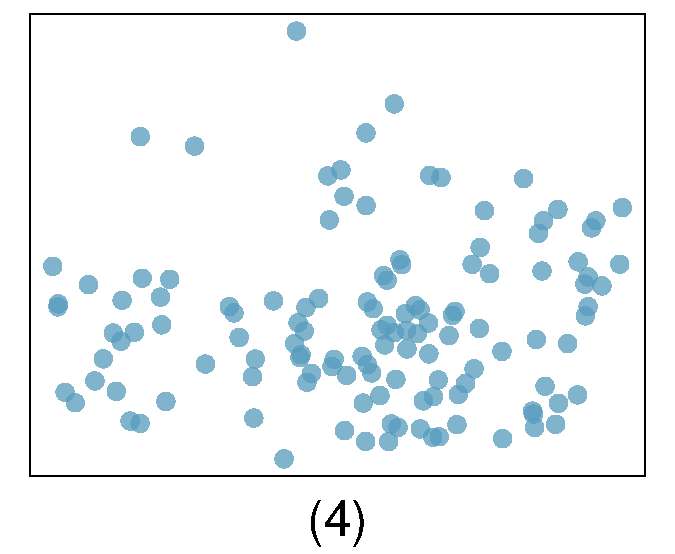
\includegraphics[width=0.245\textwidth]{ch_regr_simple_linear/figures/eoce/match_corr_3/scatter_4}
\end{minipage}
}{}

% 44 - rate_my_prof_ahss

\eoce{\qt{Rate my professor\label{rate_my_prof_ahss}}
Many college courses conclude by giving students
the opportunity to evaluate the course and the
instructor anonymously.
However, the use of these student evaluations
as an indicator of course quality and teaching
effectiveness is often criticized because these
measures may reflect the influence of
non-teaching related characteristics,
such as the physical appearance of the instructor.
Researchers at University of Texas, Austin
collected data on teaching evaluation score
(higher score means better) and standardized
beauty score (a score of 0 means average, negative
score means below average, and a positive score
means above average) for a sample of 463
professors.\footfullcite{Hamermesh:2005}
The scatterplot below shows the relationship
between these variables, and regression output
is provided for predicting teaching evaluation
score from beauty score.
\begin{center}
\begin{tabular}{rrrrr}
    \hline
            & Estimate  & Std. Error    & t value   & Pr($>$$|$t$|$) \\ 
  \hline
(Intercept) & 4.010     & 0.0255        & 	157.21  & 0.0000 \\ 
beauty      &  \fbox{\textcolor{white}{{\footnotesize Cell 1}}}  
                        & 0.0322        & 4.13      & 0.0000\vspace{0.8mm} \\ 
   \hline
\end{tabular}
\end{center}
\noindent\begin{minipage}[c]{0.45\textwidth}
{\raggedright\begin{parts}
\item
    Given that the average standardized beauty score
    is -0.0883 and average teaching evaluation score
    is 3.9983, calculate the slope.
    Alternatively, the slope may be computed using just
    the information provided in the model summary table.
\item
    Do these data provide convincing evidence that the
    slope of the relationship between teaching evaluation
    and beauty is positive?
    Explain your reasoning.
\item
    List the conditions required for linear regression
    and check if each one is satisfied for this model
    based on the following diagnostic plots.
\end{parts}}
\end{minipage}
\begin{minipage}[c]{0.07\textwidth}
$\:$ \\
\end{minipage}
\begin{minipage}[c]{0.45\textwidth}
\tabspecial{tableau-teaching-eval-beauty}{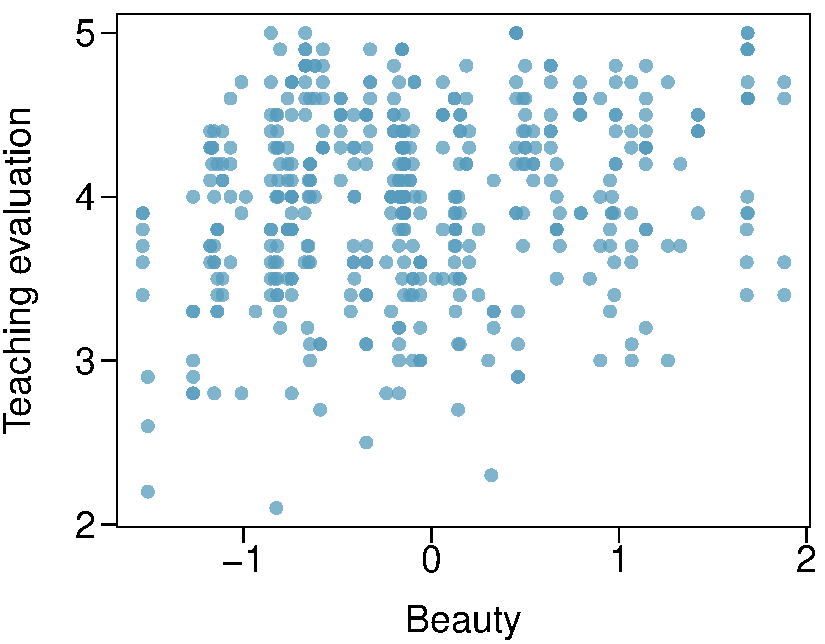
\includegraphics[width=\textwidth]{ch_regr_simple_linear/figures/eoce/rate_my_prof_ahss/rate_my_prof_eval_beauty.pdf}} \\
\end{minipage}
\begin{center}
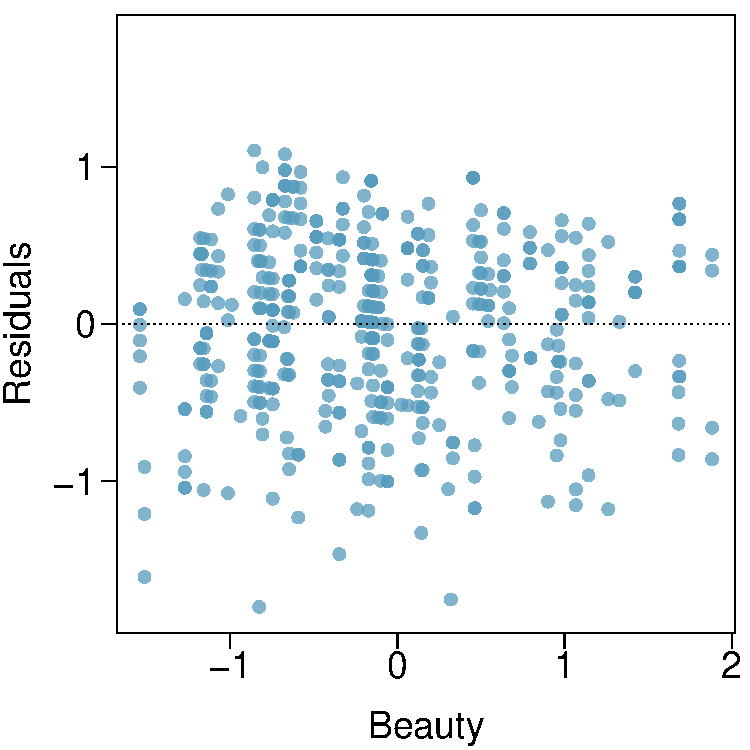
\includegraphics[width=0.32\textwidth]{ch_regr_simple_linear/figures/eoce/rate_my_prof_ahss/rate_my_prof_residuals}
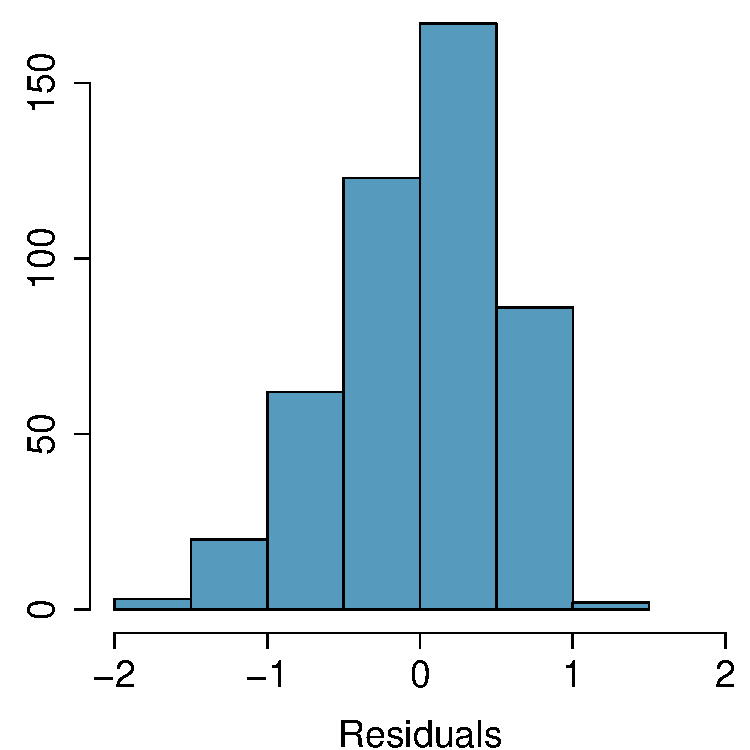
\includegraphics[width=0.32\textwidth]{ch_regr_simple_linear/figures/eoce/rate_my_prof_ahss/rate_my_prof_residuals_hist}
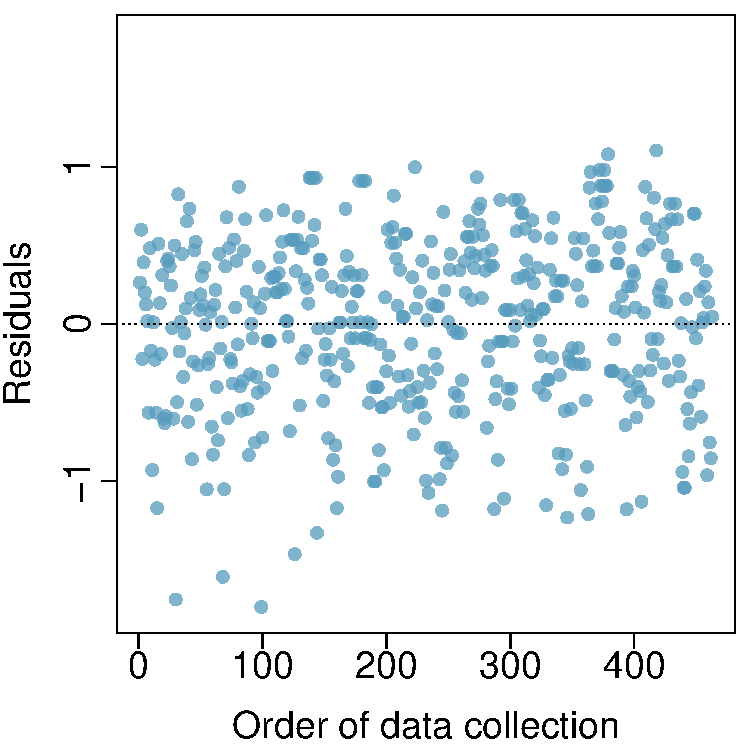
\includegraphics[width=0.32\textwidth]{ch_regr_simple_linear/figures/eoce/rate_my_prof_ahss/rate_my_prof_residuals_order}
\end{center}
}{}

\D{\newpage}

% 45 - trees_volume_height_diameter

\eoce{\qt{Trees\label{trees_volume_height_diameter}} The scatterplots below 
show the relationship between height, diameter, and volume of timber 
in 31 felled black cherry trees. The diameter of the tree is measured 
4.5 feet above the ground.\footfullcite{data:trees}
\begin{center}
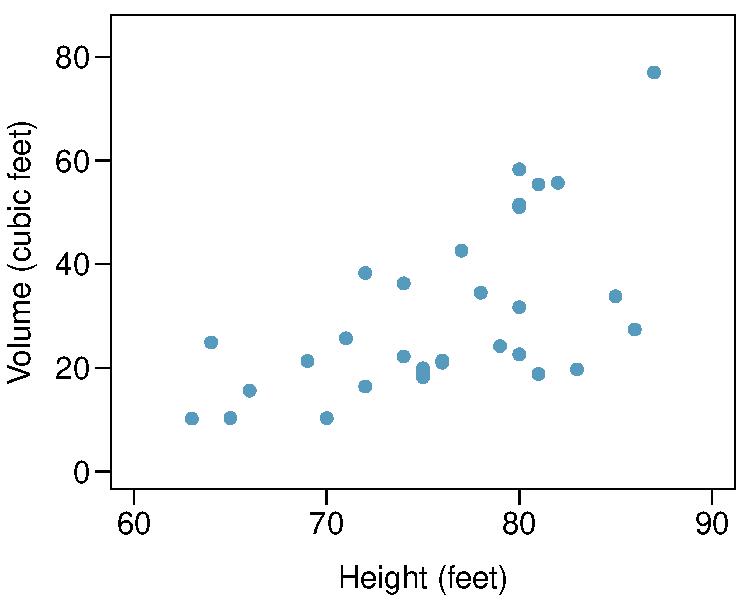
\includegraphics[width=0.46\textwidth]{ch_regr_simple_linear/figures/eoce/trees_volume_height_diameter/trees_volume_height.pdf}
\hspace{0.07\textwidth}%
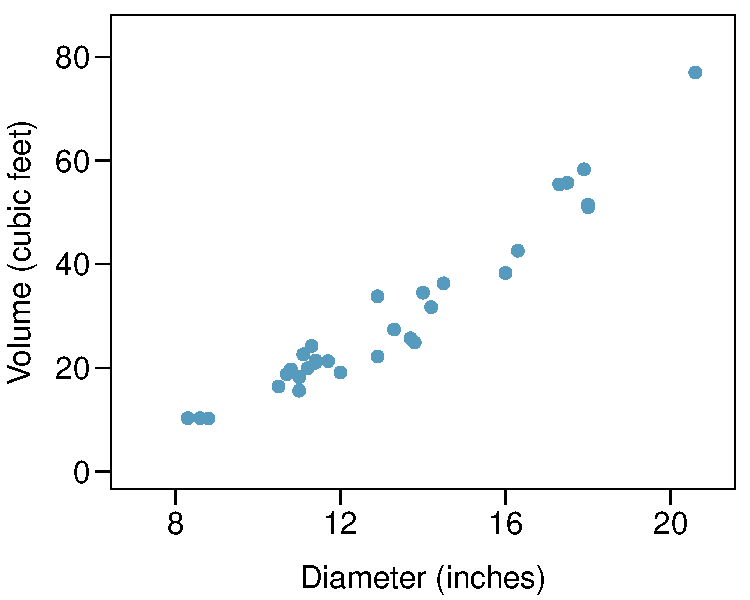
\includegraphics[width=0.46\textwidth]{ch_regr_simple_linear/figures/eoce/trees_volume_height_diameter/trees_volume_diameter.pdf}
\end{center}
\begin{parts}
\item Describe the relationship between volume and height of these trees.
\item Describe the relationship between volume and diameter of these trees.
\item Suppose you have height and diameter measurements for another black 
cherry tree. Which of these variables would be preferable to use to predict 
the volume of timber in this tree using a simple linear regression model? 
Explain your reasoning.
\end{parts}
}{}

  }



%-------------------------------------------------------------
% 5 Section Headers
%
% See headers.tex file for main chapters.
\newcommand{\chapterpagepaddingtopinner}[0]{35mm} % 45mm
\newcommand{\chapterpagepaddingbottominner}[0]{25mm}

\newcommand{\chapterXfontsize}[0]{92}
\newcommand{\chaptertitlefontsize}[0]{30}


%-------------------------------------------------------------
% 6 Utilities
% 6.1 Helpful Editing Commands
\newcommand\Add[1]{\marginpar[{\Huge\color{oiR}$\bullet$}]{\Huge\color{oiR}$\bullet$}{\color{oiB}#1}}
\newcommand\Cut[1]{\marginpar[{\Huge\color{oiR}$\bullet$}]{\Huge\color{oiR}$\bullet$}{\color{oiGC}#1}}
\newcommand\Comment[1]{\marginpar[{\Huge\color{oiR}$\bullet$}]{\Huge\color{oiR}$\bullet$} {\color{oiG}{[#1]}}}
\newcommand{\note}[1]{\Comment{#1}}
\newcommand{\commentall}[1]{}
% 6.2 Special Symbols
\newcommand{\degree}{\ensuremath{^\circ}}
\newcommand{\R}{\textbf{\textsf{R}}}
% 6.3 Text Commands (Terms, Data, Variable, Response)
\newcommand{\term}[1]{\textbf{#1}\index{#1|textbf}}
\newcommand{\termsub}[2]{\textbf{#1}\index{#2|textbf}}
\newcommand{\termni}[1]{\textbf{#1}}
\newcommand{\hiddenterm}[1]{#1\index{#1|textbf}}
\newcommand{\indexthis}[2]{#1\index{#2}}
\newcommand{\termO}[1]{\textbf{\color{termOColor}#1}}
\newenvironment{data}[1]{\texttt{#1}}{}
\newcommand{\datalink}[1]{\index{#1|textbf}\texttt{\oiRedirect{data_#1}{#1}}}
\newenvironment{var}[1]{\texttt{#1}}{}
\newenvironment{resp}[1]{\texttt{#1}}{}
\newcommand{\lmlevel}[1]{:~\emph{#1}}{}
\newenvironment{calctext}[1]{{\color{oiB}\texttt{#1}}}{}
\newenvironment{calctextmath}[1]{{\color{oiB}\mathtt{#1}}}{}
\newenvironment{calcbutton}[1]{{\color{oiB}\texttt{#1}}}{}
\newcommand{\codeindent}{\hspace{5mm}}
% 6.4 Highlighting
\newenvironment{highlight}{\textbf}{}
\newcommand{\highlightO}[1]{\textbf{\color{oiB}#1}}
\newcommand{\highlightT}[1]{\emph{\color{oiR}#1}}
% 6.5 Lengths
\setlength{\parindent}{0.3in}
% 6.6 Hyperreferences
\newcommand{\urlwofont}[1]{\urlstyle{same}\url{#1}}
%\newcommand{\oiRedirect}[2]{\href{http://www.openintro.org/redirect.php?go=#1&referrer=\referrer}{#2}}
\newcommand{\oiRedirectUrl}[1]{http://www.openintro.org/redirect.php?go=#1&referrer=ahss3_pdf}
\newcommand{\oiRedirect}[2]{\href{\oiRedirectUrl{#1}}{#2}}
\newcommand{\videoicon}[1][4.5mm]{
\includegraphics[height=#1]{extraTeX/icons/video_camera.png}~}
\newcommand{\CalculatorVideos}[1]{}%{\begin{tipBox}{\tipBoxTitle[\videoicon]{Calculator videos}
%Videos covering #1 using TI and Casio graphing calculators are available at \mbox{\oiRedirect{textbook-openintro_videos}{openintro.org/videos}}.}
%\end{tipBox}}
\newcommand{\videohref}[2][4.5mm]{\oiRedirect{#2}{\raisebox{-0.3mm}[0pt]{
\includegraphics[height=#1]{extraTeX/icons/video_camera.png}}}}
\newcommand{\tableauhref}[2][4.5mm]{\oiRedirect{#2}{\raisebox{-0.3mm}[0pt]{
\includegraphics[height=#1]{extraTeX/icons/tableau}}}}
\newcommand{\slideshref}[2][4.5mm]{\oiRedirect{#2}{\raisebox{-0.3mm}[0pt]{
\includegraphics[height=#1]{extraTeX/icons/slides.png}}}}
\newcommand{\videomarginhref}[2][4mm]{\oiRedirect{#2}{\raisebox{-3mm}[0pt]{
\includegraphics[height=#1]{extraTeX/icons/video_camera.png}}}}
\newcommand{\sectionvideohref}[2][6mm]{\oiRedirect{#2}{\raisebox{-0.5mm}[0pt]{
\includegraphics[height=#1]{extraTeX/icons/video_camera.png}}}}
\newcommand{\sectionslideshref}[2][6mm]{\oiRedirect{#2}{\raisebox{-0.5mm}[0pt]{
\includegraphics[height=#1]{extraTeX/icons/slides.png}}}}
\newcommand{\MarginVideo}[1]{\marginpar[{\videomarginhref{#1}}]{{\videomarginhref{#1}}}}
% 6.7 Helper commands
\newcommand{\us}[0]{\_\hspace{0.3mm}}
%\newcommand{\quadplus}[0]{\quad + \quad}
\newcommand{\indfunc}[2]{\var{#1}_{\resp{#2}}}


%-------------------------------------------------------------
% 7 Inference steps

\newcommand{\inferencestep}[1]{\textbf{#1}:}


%-------------------------------------------------------------
% 8 Figures and Captions
% 8.1 & 8.2 Table & Figure Numbering
% Thanks @Herbert on StackExchange for helping clean up this style code!
% http://tex.stackexchange.com/questions/176978/latex-numbering-in-counters-appears-to-have-changed/177045?noredirect=1#comment409945_177045
\makeatletter
\let\c@table\c@figure
\makeatother
% 8.3 Caption Width
\newlength{\mycaptionwidth}
\setlength{\mycaptionwidth}{0.825\textwidth}
\captionsetup{width=\mycaptionwidth}
\newcommand{\Figure}[3][]{\pdftooltip{\includegraphics[width=#2\textwidth]{\chapterfolder/figures/#3/#3}}{#1}}
\newcommand{\Figures}[4][]{\pdftooltip{\includegraphics[width=#2\textwidth]{\chapterfolder/figures/#3/#4}}{#1}}
\newcommand{\Figuress}[4][]{\pdftooltip{\includegraphics[width=#2]{\chapterfolder/figures/#3/#4}}{#1}}
\newcommand{\chapterfolder}{}


%\newcommand{\chapterfolder}{}




%-------------------------------------------------------------
% 9 Examples and Exercises
% 9.1 Exercises, within the text
% 9.1.1 Exercise Environment
\newcommand{\excolor}[1]{{\color{excolor}#1}}
\newenvironment{exercise}
{
\begin{itemize}\item[\color{oiB}$\bigodot$]\refstepcounter{equation}\noindent\normalsize\textbf{\color{oiB}Guided Practice \theexercise}%\hspace{3mm}

}
{\normalsize

\stdaddvspace{}
\end{itemize}}
% 9.1.2 Exercise Fine Tuning
\newcommand\theexercise{\thechapter.\arabic{equation}}
% 9.2 Examples
% 9.2.1 Example Environment
\newcommand\theexample{\thechapter.\arabic{equation}}
\newenvironment{example}[1]
{\begin{itemize}
\item[\color{oiB}\Large$\CIRCLE$]\refstepcounter{equation}\noindent\textbf{\color{oiB}Example \theexample}

#1\vspace{\exampleAboveBar}

{\color{examplegray}\rule{20mm}{0.1mm}}

\vspace{\exampleBelowBar}

\normalsize}{

\end{itemize}
\stdaddvspace{}
}
% 9.2.2 Wrappers
%\reversemarginpar
\def\warningsymbol{\protect\marginsymbolhelper}
\def\marginsymbolhelper{\tabto*{0mm} {\dbend} \tabto*{0mm}}
\newcommand{\exampleicon}[1]{\vspace{#1} \raggedleft
\includegraphics[width=5mm]{extraTeX/icons/example.png}\hspace{2mm}\ }
\newenvironment{gpewrapper}[1]{\addvspace{4mm}

\noindent\hspace{-12.45mm}\begin{minipage}[c]{\textwidth+8mm}
\begin{minipage}[c]{8.4mm}
\hspace{0.5mm}\includegraphics[width=5mm]{extraTeX/icons/#1.png}
\end{minipage}\begin{minipage}[c]{\textwidth-0.45mm}\begin{mdframed}[%
    topline=false,
    rightline=false,
    bottomline=false,
    linewidth=0.5mm,
    linecolor=oiB]}{\end{mdframed}\end{minipage}\end{minipage}

    \addvspace{4mm}}
\newenvironment{examplewrap}
    {\begin{gpewrapper}{example}}
    {\end{gpewrapper}}
\newenvironment{exercisewrap}
    {\begin{gpewrapper}{guided_practice}}
    {\end{gpewrapper}}
% 9.2.3 Example Title
\newcommand{\exampletitle}[1]{\textbf{\color{oiB}\small\fontfamily{phv}%
\selectfont{\MakeUppercase{Example~#1}}} \\[1mm]}
\newcommand{\exercisetitle}[1]{\textbf{\color{oiB}\small\fontfamily{phv}%
\selectfont{\MakeUppercase{Guided Practice~#1}}} \\[1mm]}

% 9.2.4 NEW Example and Guided Practice Environment
\newcommand{\exspace}{\stdvspace{}}
\newenvironment{nexample}[1]{\addvspace{6mm}

\refstepcounter{equation}\exampletitle{\theexample}
Example problem: #1

\addvspace{\nexampleAboveBar}

{\color{examplegray}\rule{20mm}{0.1mm}}

\addvspace{\nexampleBelowBar}

\setlength{\parskip}{2mm}Solution to the example:}{

\MakeUppercase{Example~\theexample{} Has Ended.}}
\newenvironment{nexercise}{\addvspace{6mm}

\refstepcounter{equation}\exercisetitle{\theexample}}{ Go to the preceding footnote link for the Guided Practice solution.

\MakeUppercase{Guided Practice~\theexample{} Has Ended.}}

% 9.3 EOCEs: End of Chapter Exercises
% 9.3.1 Environment
\newenvironment{eoce}[2][]
{\refstepcounter{eoce}\noindent\small\textbf{\textcolor{oiB}{{\hypersetup{linkcolor=oiB}{\fontfamily{phv}\selectfont\ref{eoce_sol_\arabic{chapter}_\arabic{eoce}}}}\label{eoce_\arabic{chapter}_\arabic{eoce}}}}\hspace{2mm} #1#2

\addvspace{4mm}

}
%{\em #2 } $\:$ \\ }
{}
% 9.3.2 EOCE Solutions
\newcommand{\eocesolch}[1]{
\refstepcounter{eocesolch}\noindent\textbf{\color{oiB}\arabic{eocesolch}\hspace{2mm}#1}

\addvspace{2mm}

}
{
\newcommand{\eocesol}[1]{\refstepcounter{eocesol}\noindent\textbf{\color{oiB}{\hypersetup{linkcolor=oiB}{\fontfamily{phv}\selectfont\ref{eoce_\arabic{eocesolch}_\arabic{eocesol}}}}\label{eoce_sol_\arabic{eocesolch}_\arabic{eocesol}}}\hspace{2mm}{\small#1}\makebox[0pt]{\color{white}\tiny \refstepcounter{eocesol}\label{eoce_sol_\arabic{eocesolch}_\arabic{eocesol}}}

\addvspace{1mm}

}
% 9.3.3 EOCE Utilities
\newcommand{\qt}[2][.]{{\fontfamily{phv}\selectfont\textcolor{oiB}{\textbf{#2#1}}}}
\newcommand{\qtq}[1]{{\fontfamily{phv}\selectfont\textcolor{oiB}{\textbf{#1?}}}}
\newcommand{\ec}[1]{\textcolor{oiB}{\footnotesize{~(#1)}}}% 9.3.4 EOCE Roman Parts
\newenvironment{romanparts}{
\begin{enumerate}[I.]
\setlength{\itemsep}{0mm}
}{\end{enumerate}}
% 9.3.5 EOCE Parts
\newenvironment{parts}{
%\vspace{-0.25cm}
\begin{enumerate}[(a)]
\setlength{\itemsep}{0mm}}
{\end{enumerate}}
% 9.3.6 EOCE Subparts
\newenvironment{subparts}{
\begin{enumerate}[i.]
\setlength{\itemsep}{0mm}}
{\end{enumerate}}
% 9.3.7 EOCE hyp environment
\newenvironment{hyp}{
\begin{itemize}
\setlength{\itemsep}{0mm}
}
{\end{itemize}
}
% 9.3.8 cond environment
\newenvironment{cond}{
\begin{enumerate}[1.]
\setlength{\itemsep}{0mm}
}
{\end{enumerate}
}
% 9.3.9 Exercise fixes required.
\newcommand{\eoceNeedSolution}[1][]
{\textbf{\refstepcounter{eoceNeedSolution} \color{red}ADD SOLUTION. #1}}
\newcommand{\eoceReplace}[1][]
{\textbf{\refstepcounter{eoceReplace} \color{red}REPLACE THIS EXERCISE. #1}}
\newcommand{\eoceFF}[1][]
{\textbf{\refstepcounter{eoceFF} \color{red}FINAL FORMATTING.}}





%-------------------------------------------------------------
% 10 Special Boxes
% 10.1.1 Term Box
\newcommand\tBoxTitleBuffer{\\[1.5mm]}
\newenvironment{tBoxTitle}[2][\tBoxTitleBuffer]{\textbf{\color{oiB}#2} #1
}{}
\newenvironment{termBox}[1]{
\addvspace{4mm}
\noindent{\color{oiB}\framebox[\textwidth][c]{\framebox[\textwidth-3mm][l]{ \\
	\vspace{0.5cm} \\
	\begin{minipage}[b]{\textwidth-3mm}
		\begin{minipage}[t]{2mm}
			\hspace{2mm}
		\end{minipage}
		\begin{minipage}[b]{\textwidth-10mm}
			\color{black}\ \\[-0.7mm]
			#1
			
			\vspace{1mm}
		\end{minipage}
	\end{minipage}}}}
}{

\addvspace{1mm}}
% 10.2 Tip Box
\newenvironment{tipBoxTitle}[2][TIP:\ ]{\textbf{\color{oiB}#1#2}\\[0.3mm]}{}
\newenvironment{tipBox}[1]{
\addvspace{4mm}
\noindent{\color{oiB}\framebox[\textwidth][l]{ \\
	\vspace{5mm} \\
	\begin{minipage}[b]{\textwidth-4mm}
		\begin{minipage}[t]{2mm}
			\hspace{2mm}
		\end{minipage}
		\begin{minipage}[b]{\textwidth-8mm}
			\color{black}\ \\[-0.7mm]
			#1
			
			\vspace{1mm}
		\end{minipage}
	\end{minipage}}}
}{

\addvspace{1mm}}
% 10.3 Caution Box
\newenvironment{caution}[2]{
\addvspace{4mm}
\noindent{\color{oiB}\framebox[\textwidth][l]{ \\
	\vspace{5mm} \\
	\begin{minipage}[b]{\textwidth-4mm}
		\begin{minipage}[t]{2mm}
			\hspace{2mm}
		\end{minipage}
		\begin{minipage}[b]{\textwidth-8mm}
			\textbf{\color{oiB}Caution: #1} \\[1mm]
			\color{black}#2
		\end{minipage}
	\end{minipage}}}
}{

\addvspace{1mm}}
% 10.4 One Box
\newenvironment{onebox}[1]{
\addvspace{4mm}
\noindent\begin{minipage}{\textwidth}
\noindent\rule{\textwidth}{0.3pt}\vspace{-6mm}
\begin{mdframed}[%
    topline=false,
    rightline=false,
    leftline=false,
    bottomline=false,
    backgroundcolor=grayBackground]
\textbf{\color{oiB}\small\fontfamily{phv}%
\selectfont{\MakeUppercase{#1}}} \\[1mm]}{
\end{mdframed}\vspace{-4.2mm}
\rule{\textwidth}{0.3pt}
\end{minipage}

\addvspace{4mm}}

%% exercise tags
 \newcommand{\tabspecial}[2]{\oiRedirect{#1}{#2\tableauhref{#1}}}
\newcommand{\videosolution}[1]{\videohref{#1}\ \ }






%
% Tablet Version
\setlength\paperheight{8.82in}
\setlength\textheight{8.25in}
\setlength\paperwidth{5.7in}
\setlength\textwidth{5.45in}
\setlength\voffset{-23.5mm}
\setlength\hoffset{-27mm}
\setlength\oddsidemargin{5mm}
\setlength\evensidemargin{5mm}
\setlength{\marginparsep}{5mm}
\setlength{\marginparwidth}{35mm}


%\include{extraTeX/style/video}
% The following style file supports an 8.25 x 11 paper size.
%\include{extraTeX/style/hardcover}

%\title{\huge Advanced High School Statistics\vspace{1.5mm} \\ \Large Second Edition,\\ with updates based on AP$^{\text{\textregistered}}$ Statistics Course Framework}
%\author{David Diez \\
%\small\emph{Data Scientist}\\
%\small\emph{OpenIntro} \\[6mm]
%Mine \c{C}etinkaya-Rundel \\
%\small\emph{Associate Professor of the Practice,
%    Duke University} \\
%\small\emph{Professional Educator, RStudio} \\[6mm]
%Leah Dorazio \\
%\small\emph{Statistics and Computer Science Teacher}\\
%\small\emph{San Francisco University High School} \\[6mm]
%Christopher D Barr \\
%\small\emph{Investment Analyst} \\
%\small\emph{Varadero Capital} \\
%}
%_derivative}
\date{}
\renewcommand\contentsname{Table of Contents}
%\setcounter{tocdepth}{1} % standard version
\setcounter{tocdepth}{3} % screen reader version
%\renewcommand{\cftchapfont}{\scshape}
%\renewcommand{\cftsecfont}{\bfseries}

\begin{document}
%\include{extraTeX/preamble/review_copy}
\renewcommand{\thepage}{}
\maketitle
\chapter*{}

\vfill

\noindent Copyright $\copyright$ 2015 OpenIntro, Inc. First Edition. \\
Updated: \versiondate. \\

\noindent This textbook is available under a Creative Commons license. % Attribution-ShareAlike license. \\
Visit \oiRedirect{textbook-openintro_textbook}{openintro.org} for a free PDF, to download the textbook's source files, or for more information about the license. \\

%\noindent Modified versions of this textbook, including reformatted electronic versions, may not be redistributed under a title that suggests association with or endorsement by OpenIntro, e.g. it cannot be titled \emph{OpenIntro Statistics}. %More information on branding restrictions for derivatives is available on the Rights page at~\href{http://www.openintro.org/rights.php}{openintro.org}.

\noindent {\scriptsize AP\textregistered{} is a trademark registered and owned by the College Board, which was not involved in the production of, and does not endorse, this product.}
%_derivative}
\renewcommand{\thepage}{\arabic{page}}
\tableofcontents
\chapter*{{\color{oiB}Preface}\vspace{-6mm}}

\noindent%
\emph{Advanced High School Statistics} covers a first course in statistics, providing an introduction to applied statistics that is clear, concise, and accessible. This book was written to align with the AP$^{\text{\textregistered}}$ Statistics Course
Description\footnote{AP$^{\text{\textregistered}}$ is
  a trademark registered and owned by the College Board,
  which was not involved in the production of, and does
  not endorse, this product.
  \oiRedirect{collegeboard-ap_statistics_course_description}
      {apcentral.collegeboard.org/pdf/ap-statistics-course-description.pdf}}, but it's also popular in non-AP courses and community colleges.
\vspace{3mm}

\noindent%
This book may be downloaded as a free PDF at
\oiRedirect{ahss}{\color{black}\textbf{openintro.org/ahss}}.
\vspace{3mm}

\noindent%
We hope readers will take away three ideas from this book in addition to forming a foundation of statistical thinking and methods.\vspace{-1mm}
\begin{enumerate}
\setlength{\itemsep}{0mm}
\item[(1)] Statistics is an applied field with a wide range of practical applications.
\item[(2)] You don't have to be a math guru to learn from real, interesting data.
\item[(3)] Data are messy, and statistical tools are imperfect. But, when you understand the strengths and weaknesses of these tools, you can use them to learn about the real~world.
\end{enumerate}


\subsection*{{\color{oiB}Textbook overview}}

The chapters of this book are as follows:
\begin{description}
\setlength{\itemsep}{0mm}
\item[1. Data collection.] Data structures, variables, and basic data collection techniques; experimental designs and sampling methods are presented and compared.
\item[2. Summarizing data.] Data summaries and graphics;  includes normal approximation for data.
\item[3. Probability and probability distributions.] The basic principles of probability and random variables, as well as an introduction to the geometric and binomial distributions.
\item[4. Sampling distributions.] Sampling distributions for a sample proportion and a sample mean; also includes distributions for a difference of sample means and a difference of sample proportions.
\item[5. Foundations for inference.] General ideas for statistical inference in the context of estimating the population proportion.
\item[6. Inference for categorical data.]
    Inference for proportions and contingency tables
    using the normal and chi-square distributions.
\item[7. Inference for numerical data.]
    Inference for one or two sample means using the
    $t$-distribution.
\item[8. Introduction to linear regression.] An introduction to regression with two variables; includes inference on the slope of the regression line.
\end{description}

\subsection*{{\color{oiB}Online resources}}
OpenIntro is focused on increasing access to education by developing free,
high-quality education materials.
In addition to textbooks, we provide the following free resources
to help teachers and students be successful on our website.

\begin{itemize}
\setlength{\itemsep}{0mm}
\item Video overviews for each section of the textbook
\item Lecture slides for each section of the textbook
\item \oiRedirect{casio_all}{Casio} and \oiRedirect{ti_all}{TI} calculator tutorials
\item \oiRedirect{ahss-solutions}{Video solutions} for selected section and chapter exercises
\item Statistical software labs
\item A small but growing number of \oiRedirect{ahss-desmos}{Desmos activities}\footnote{\oiRedirect{ahss-desmos}{openintro.org/ahss/desmos}}
\item \oiRedirect{ahss-quizlet}{Quizlet} sets for each chapter\footnote{\oiRedirect{ahss-quizlet}{quizlet.com/openintro-ahss}}
\item A \oiRedirect{ahss-tableau}{Tableau public} page to further interact with data sets\footnote{\oiRedirect{ahss-tableau}{public.tableau.com/profile/openintro}}
%\item \oiRedirect{ahss2-online-temp}{Online, interactive version of textbook}\footnote{Developed by Emiliano Vega and Ralf Youtz of Portland Community College using PreTeXt.}
\item Complete companion course with the learning management software \oiRedirect{ahss_mom}{{MyOpenMath}}\footnote{\oiRedirect{myopenmath-ahss}{myopenmath.com/course/public.php?cid=11774}}
\item Complete Canvas course accessible through \oiRedirect{ahss_canvas}{{Canvas Commons}}\footnote{\oiRedirect{canvas_course-sfuhs}{sfuhs.instructure.com/courses/1068}}
\end{itemize}

\noindent%
All of these resources can be found at: 
\begin{center}
\oiRedirect{ahss}
    {\color{black}\textbf{openintro.org/ahss}}
\end{center}

\noindent%	
We also have improved the ability to access data in this book
through the addition of Appendix~\ref{appendix_data},
which provides additional information for each of the data sets
used in the main text.
Online guides to each of these data sets are also provided at
\oiRedirect{data}
    {\color{black}\textbf{openintro.org/data}}
and through a
\oiRedirect{textbook-github_openintro}
    {companion R~package}.

% Official:
% http://www.openintro.org/package/openintro
% Currently redirect it to:
% http://openintrostat.github.io/openintro-r-package/
\vspace{3mm}

\subsection*{{\color{oiB}Examples and exercises}}
%, and appendices}

\noindent%
Many examples are provided to establish an understanding of how
to apply methods.

\begin{examplewrap}
\begin{nexample}{This is an example.}
  Full solutions to examples are provided here, within the example.
\end{nexample}
\end{examplewrap}

\noindent%
When we think the reader should be ready to try an example problem
on their own, we frame it as Guided Practice.

\begin{exercisewrap}
\begin{nexercise}
The reader may check or learn the answer to any Guided Practice
problem by reviewing the full solution in a footnote.\footnotemark{}
%Readers are strongly encouraged to attempt these practice problems.
\end{nexercise}
\end{exercisewrap}
\footnotetext{Guided Practice solutions are always located down here!}

\noindent%
Exercises are also provided at the end of each section
and each chapter for practice or homework assignments.  
Solutions for odd-numbered exercises are given in
Appendix~\ref{eoceSolutions}.

\subsection*{{\color{oiB}Getting involved}}
We encourage anyone learning or teaching statistics to visit
\oiRedirect{textbook-openintro}
    {\color{black}\textbf{openintro.org}}
and get involved.
We~also value your feedback.
%Please send any questions or comments to \href{mailto:leah@openintro.org}{leah@openintro.org}.
Please provide feedback, report typos, and review known typos at
\begin{center}
\oiRedirect{ahss_feedback}
    {\color{black}\textbf{openintro.org/ahss/feedback}}
\end{center}


\subsection*{{\color{oiB}Acknowledgements}}

This project would not be possible without the passion
and dedication of all those involved.
The authors would like to thank the
\oiRedirect{textbook-openintro_about}{OpenIntro Staff}
for their involvement and ongoing contributions.
We~are also very grateful to the hundreds of students
and instructors who have provided us with valuable feedback
since we first started working on this project in~2009.
A special thank you to Stephen Miller and Juan Gomez for reviewing and providing feedback on the third edition of AHSS.





\normalsize

\begingroup
%-------------------------------------------------------------
% 5 Section Headers

% 5.0 Spacings
\newcommand{\chapterpagepadding}[0]{7mm}
\newcommand{\sectionheaderspaceA}{1mm}
\newcommand{\sectionheaderspaceB}{4mm}
\newcommand{\sectionheaderspaceC}{2mm}
\newcommand{\sectionheaderspaceD}{6mm}
\newcommand{\setupfont}
    {\normalfont\LARGE\bfseries\fontfamily{phv}\selectfont}
\newcommand{\setupfontsectionexercises}
    {\normalfont\bfseries\fontfamily{phv}\selectfont}
\newcommand{\setfontsize}[1]{\fontsize{#1}{#1}\selectfont}

% 5.1 Chapter
\newcommand{\titlebreak}[1][5mm]{\\[#1]}
\newcommand{\chaptertitle}[2][\chaptertitlefontsize]{{\color{white}\titlerule[1.5mm]}\addvspace{\sectionheaderspaceB}
    {\setupfont{}\color{chaptertitlegray}\setfontsize{#1}#2} \\[2mm]
        {\color{white}\titlerule[1.5mm]}

~\vspace{15mm}

}
\titleformat{\chapter}[display]
{\color{oiB}\normalfont\Huge\bfseries\raggedright}{\chaptertitlename\
\thechapter}{20pt}{{\setupfont{}\Huge #1}}
\newenvironment{chapterpage}[1]{
%\newpage
\noindent\begin{fullminipage}[left=\chapterpagepadding{},right=\chapterpagepadding{},top=\chapterpagepadding{},bottom=\chapterpagepadding{},bgcolor=seaBackground]
%\noindent\rule{\textwidth}{0.3pt}\vspace{-6mm}
\begin{mdframed}[%
    topline=false,
    rightline=false,
    leftline=false,
    bottomline=false,
    innerleftmargin=\chapterpagepaddinginner{},
    innerrightmargin=\chapterpagepaddingrightinner{},
    innertopmargin=\chapterpagepaddingtopinner{},
    innerbottommargin=\chapterpagepaddinginner{},
    backgroundcolor=seaBackground]
\chapter{#1}%{\pagewidth-10mm}
%\textbf{\color{oiB}\small\fontfamily{phv}%
%\selectfont{\MakeUppercase{#1}}} \\[1mm]
}{
\end{mdframed}
%\rule{\textwidth}{0.3pt}
\end{fullminipage}}
\titleformat{\chapter}
    {}
    {\setupfont{}\setfontsize{\chapterXfontsize}\color{oiB}Chapter~\thechapter}% \quad #1}
    {1em}
    {}
    []
\titlespacing{\chapter}
   {0pt}% left
   {0pt}% before sep
   {\baselineskip}% after sep% 5.3 Subsection
\newcommand{\chaptersection}[1]{\Large\fontfamily{phv}%
\selectfont\textbf{\ref{#1}~\nameref{#1}} \\[4mm]}

% 5.1.1 Chapter introduction
\newcommand{\chapterintro}[1]{
  %\fancyhead[RO,LE]{\thepage}
  \fancyhead[RE]{}
  \fancyhead[LO]{}

  ~\vspace{25mm}

  {\color{oiB}\titlerule[1.5mm]}\addvspace{7mm}

  {\large
  \begingroup\onehalfspacing
  \noindent%
  #1\vspace{7mm}\par
  \endgroup}

  {\color{oiB}\titlerule[0.5mm]}

  \vfill

  \noindent%
  \oiRedirect{stat}{
\includegraphics[height=10mm]{extraTeX/icons/video_and_slides.png}}
  \vspace{5mm}

  {\color{oiB}\titlerule[0.5mm]}
  
  ~\vspace{5mm}
  
  {\Large\noindent%
  For videos, slides, and other resources, please visit \\[2mm]
  \oiRedirect{ahss}
      {\textbf{\color{oiB}www.openintro.org/ahss}}}%
      \vspace{5mm}

  ~\newpage
  %\fancyhead[RO,LE]{\thepage}
  \fancyhead[RE]{\leftmark}
  \fancyhead[LO]{\rightmark}
}

% 5.2 Section
\newcommand{\clearpageforsection}{\clearpage}
\let\oldsection\section
\renewcommand\section{\clearpageforsection\oldsection}
\titleformat{\section}
    {{\color{oiR}\titlerule[1mm]}\addvspace{\sectionheaderspaceA}\color{oiB}\setupfont{}}
    {\color{oiB}\thesection \quad #1}
    {1em}
    {}
    [{\color{oiR}\titlerule[1mm]}\addvspace{4mm}]
\titlespacing{\section}
   {0pt}% left
   {0pt}% before sep
   {\baselineskip}% after sep% 5.3 Subsection
\titleformat{\subsection}
    {{\color{grayDark}\titlerule[0.1mm]}\vspace{2mm}\color{oiB}\normalfont\large%
        \bfseries\fontfamily{phv}%
        \selectfont}
    {\color{oiB}\thesubsection}
    {1em}
    {#1}
\titlespacing{\subsection}
   {0pt}% left
   {8mm}% before sep
   {\baselineskip}% after sep% 5.3 Subsection
\newcommand{\reviewheader}[1]
  {
    \clearpageforsection
    {{\color{oiR}\titlerule[1mm]}%
        \vspace*{\sectionheaderspaceC}
    \noindent\setupfont{}\color{oiB}#1 \\[-1mm]
    {\color{oiR}\titlerule[1mm]} \\[2mm]
    }
    \setcounter{secnumdepth}{0}
    \addcontentsline{toc}{section}{#1}
    \setcounter{secnumdepth}{2}
}
\newcommand{\reviewchapterheader}[1][Chapter highlights]
  {
    \reviewheader{#1}
  }


% 5.4 Section Introduction
\newcommand{\sectionintro}[1]{\begin{spacing}{1.1}\large
#1
\end{spacing}}
\newcommand{\nsubsection}[1]{\subsection{\MakeUppercase{#1}}}


% 5.5 Review Exercises
\newcommand{\reviewexercisesheader}[1][Chapter exercises]
  {\reviewheader{#1}
  }
\newcommand{\exercisesheader}[1][Exercises]
  {
    \clearpageforsection
    {{\color{oiR}\titlerule[1.0mm]}%
        \vspace*{\sectionheaderspaceC}
    \noindent\setupfont{}\large\color{oiB}\textbf{#1}
    } \vspace*{\sectionheaderspaceD{}}
  }

%%-------------------------------------------------------------
% 5 Section Headers

% 5.0 Spacings
\newcommand{\chapterpagepadding}[0]{7mm}
\newcommand{\sectionheaderspaceA}{1mm}
\newcommand{\sectionheaderspaceB}{4mm}
\newcommand{\sectionheaderspaceC}{2mm}
\newcommand{\sectionheaderspaceD}{6mm}
\newcommand{\setupfont}
    {\normalfont\LARGE\bfseries\fontfamily{phv}\selectfont}
\newcommand{\setupfontsectionexercises}
    {\normalfont\bfseries\fontfamily{phv}\selectfont}
\newcommand{\setfontsize}[1]{\fontsize{#1}{#1}\selectfont}

% 5.1 Chapter
\newcommand{\titlebreak}[1][5mm]{\\[#1]}
\newcommand{\chaptertitle}[2][\chaptertitlefontsize]{{\color{white}\titlerule[1.5mm]}\addvspace{\sectionheaderspaceB}
    {\setupfont{}\color{chaptertitlegray}\setfontsize{#1}#2} \\[2mm]
        {\color{white}\titlerule[1.5mm]}

~\vspace{15mm}

}
\titleformat{\chapter}[display]
{\color{oiB}\normalfont\Huge\bfseries\raggedright}{\chaptertitlename\
\thechapter}{20pt}{{\setupfont{}\Huge #1}}
\newenvironment{chapterpage}[1]{
%\newpage
\noindent\begin{fullminipage}[left=\chapterpagepadding{},right=\chapterpagepadding{},top=\chapterpagepadding{},bottom=\chapterpagepadding{},bgcolor=seaBackground]
%\noindent\rule{\textwidth}{0.3pt}\vspace{-6mm}
\begin{mdframed}[%
    topline=false,
    rightline=false,
    leftline=false,
    bottomline=false,
    innerleftmargin=\chapterpagepaddinginner{},
    innerrightmargin=\chapterpagepaddingrightinner{},
    innertopmargin=\chapterpagepaddingtopinner{},
    innerbottommargin=\chapterpagepaddinginner{},
    backgroundcolor=seaBackground]
\chapter{#1}%{\pagewidth-10mm}
%\textbf{\color{oiB}\small\fontfamily{phv}%
%\selectfont{\MakeUppercase{#1}}} \\[1mm]
}{
\end{mdframed}
%\rule{\textwidth}{0.3pt}
\end{fullminipage}}
\titleformat{\chapter}
    {}
    {\setupfont{}\setfontsize{\chapterXfontsize}\color{oiB}Chapter~\thechapter}% \quad #1}
    {1em}
    {}
    []
\titlespacing{\chapter}
   {0pt}% left
   {0pt}% before sep
   {\baselineskip}% after sep% 5.3 Subsection
\newcommand{\chaptersection}[1]{\Large\fontfamily{phv}%
\selectfont\textbf{\ref{#1}~\nameref{#1}} \\[4mm]}


% 5.1.1 Chapter introduction
\newcommand{\chapterintro}[1]{
%  \fancyhead[RE]{}
%  \fancyhead[LO]{}

%  ~\vspace{25mm}

%  {\color{oiB}\titlerule[1.5mm]}\addvspace{7mm}

%  {\Large
%  \begingroup\onehalfspacing
%  \noindent%
  #1%\vspace{7mm}\par
%  \endgroup}

%  {\color{oiB}\titlerule[0.5mm]}

  \vfill

  \noindent%
  \oiRedirect{stat}{
\includegraphics[height=10mm]{extraTeX/icons/video_and_slides.png}}
  \vspace{5mm}

%  {\color{oiB}\titlerule[0.5mm]}
  
%  ~\vspace{5mm}
  
  {\Large\noindent%
  For videos, slides, and other resources, please visit \\[2mm]
  \oiRedirect{ahss}
      {\textbf{\color{oiB}www.openintro.org/ahss}}}%
      \vspace{5mm}

  ~\newpage
  %\fancyhead[RO,LE]{\thepage}
%  \fancyhead[RE]{\leftmark}
%  \fancyhead[LO]{\rightmark}
}


% 5.2 Section
\newcommand{\clearpageforsection}{\clearpage}
\let\oldsection\section
\renewcommand\section{\clearpageforsection\oldsection}
\titleformat{\section}
    {{\color{oiR}\titlerule[1mm]}\addvspace{\sectionheaderspaceA}\color{oiB}\setupfont{}}
    {\color{oiB}\thesection \quad #1}
    {1em}
    {}
    [{\color{oiR}\titlerule[1mm]}\addvspace{4mm}]
\titlespacing{\section}
   {0pt}% left
   {0pt}% before sep
   {\baselineskip}% after sep% 5.3 Subsection
\titleformat{\subsection}
    {{\color{grayDark}\titlerule[0.1mm]}\vspace{2mm}\color{oiB}\normalfont\large%
        \bfseries\fontfamily{phv}%
        \selectfont}
    {\color{oiB}\thesubsection}
    {1em}
    {#1}
\titlespacing{\subsection}
   {0pt}% left
   {8mm}% before sep
   {\baselineskip}% after sep% 5.3 Subsection
\newcommand{\reviewheader}[1]
  {
    \clearpageforsection
    {{\color{oiR}\titlerule[1mm]}%
        \vspace*{\sectionheaderspaceC}
    \noindent\setupfont{}\color{oiB}#1 \\[-1mm]
    {\color{oiR}\titlerule[1mm]} \\[2mm]
    }
    \setcounter{secnumdepth}{0}
    \addcontentsline{toc}{section}{#1}
    \setcounter{secnumdepth}{2}
}
\newcommand{\reviewchapterheader}[1][Chapter highlights]
  {
    \reviewheader{#1}
  }


% 5.4 Section Introduction
\newcommand{\sectionintro}[1]{\begin{spacing}{1.1}
%\large
#1\end{spacing}
}
\newcommand{\nsubsection}[1]{\subsection{\MakeUppercase{#1}}}


% 5.5 Review Exercises
\newcommand{\reviewexercisesheader}[1][Chapter exercises]
  {\reviewheader{#1}
  }
\newcommand{\exercisesheader}[1][Exercises]
  {
    \clearpageforsection
    {{\color{oiR}\titlerule[1.0mm]}%
        \vspace*{\sectionheaderspaceC}
    \noindent\setupfont{}\large\color{oiB}\textbf{#1}
    } \vspace*{\sectionheaderspaceD{}}
  }


\includechapter{1}{ch_data_collection}
\includechapter{2}{ch_summarizing_data}
\includechapter{3}{ch_probability}
\includechapter{4}{ch_distributions}
\includechapter{5}{ch_foundations_for_inf}
\includechapter{6}{ch_inference_for_props}
\includechapter{7}{ch_inference_for_means}
\includechapter{8}{ch_regr_simple_linear}
\endgroup


\begingroup
\newcommand{\clearpageforsection}{\addvspace{8mm}

}
\fancyhead[LO]{}

\appendix{}
\addtocontents{toc}{\protect\setcounter{tocdepth}{0}}
\chapter{Exercise solutions}
\label{eoceSolutions}





%_______________
\eocesolch{Data collection}



%_______________
\begin{multicols}{2}

% 1 - migraine_and_acupuncture_intro

\eocesol{(a)~Treatment: $10/43 = 0.23 \rightarrow 23\%$. 
(b)~Control: $2/46 = 0.04 \rightarrow 4\%$. 
(c)~A higher percentage of patients in the treatment group were pain 
free 24 hours after receiving acupuncture. 
(c)~It is possible that the observed difference between the two group 
percentages is due to chance.}

% 3 - study_components_airpoll

\eocesol{(a)~``Is there an association between air pollution exposure and preterm births?"
(b)~143,196 births in Southern California between 1989 and 1993.
(c)~Measurements of carbon monoxide, nitrogen dioxide, ozone, and particulate 
matter less than 10$\mu g/m^3$ (PM$_{10}$) collected at air-quality-monitoring 
stations as well as length of gestation. Continous numerical variables. }

% 5 - study_components_cheaters

\eocesol{(a)~``Does explicitly telling children not to cheat affect their likelihood to 
cheat?".
(b)~160 children between the ages of 5 and 15.
(c)~Four variables: (1) age (numerical, continuous), (2) sex (categorical), 
(3) whether they were an only child or not (categorical), (4) whether they 
cheated or not (categorical).}

% 7 - migraine_and_acupuncture_exp_resp

\eocesol{Explanatory: acupuncture or not.
Response: if the patient was pain free or not.}

% 9 - fisher_irises

\eocesol{(a)~$50 \times 3 = 150$. 
(b)~Four continuous numerical variables: sepal length, sepal width, petal length, and petal width. 
(c)~One categorical variable, species, with three levels: \emph{setosa}, \emph{versicolor}, and \emph{virginica}.}

% 11 - airports

\eocesol{(a)~Airport ownership status (public/private),
    airport usage status (public/private),
    latitude,
    and longitude.
(b)~Airport ownership status: categorical, not ordinal.
    Airport usage status: categorical, not ordinal.
    Latitude: numerical, continuous.
    Longitude: numerical, continuous.}

% 13 - scope_airpoll

\eocesol{(a)~Population: all births, sample: 143,196 births between 1989 and 1993 in 
Southern California. 
(b)~If births in this time span at the geography can be considered to be 
representative of all births, then the results are generalizable to the 
population of Southern California. However, since the study is observational 
the findings cannot be used to establish causal relationships.}

% 15 - scope_buteyko

\eocesol{(a)~Population: all asthma patients aged 18-69 who rely on medication for 
asthma treatment. Sample: 600 such patients.
(b)~If the patients in this sample, who are likely not randomly sampled, can 
be considered to be representative of all asthma patients aged 18-69 who rely 
on medication for asthma treatment, then the results are generalizable to the 
population defined above. Additionally, since the study is experimental, the 
findings can be used to establish causal relationships.}

% 17 - relax_after_work_definitions

\eocesol{(a)~Observation.
(b)~Variable.
(c)~Sample statistic (mean).
(d)~Population parameter (mean).}

% 19 - course_satisfaction_sections

\eocesol{(a)~Observational.
(b)~Use stratified sampling to randomly sample a fixed number of students, 
say 10, from each section for a total sample size of 40 students.}

% 21 - internet_life_expectancy

\eocesol{(a)~Positive, non-linear, somewhat strong. Countries in which a higher 
percentage of the population have access to the internet also tend to have 
higher average life expectancies, however rise in life expectancy trails 
off before around 80 years old.
(b)~Observational.
(c)~Wealth: countries with individuals who can widely afford the internet 
can probably also afford basic medical care. (Note: Answers may vary.)}

% 23 - evaluate_sampling_methods

\eocesol{(a)~Simple random sampling is okay. In~fact, it's rare for simple random 
sampling to not be a reasonable sampling method! 
(b)~The student opinions may vary by field of study, so the stratifying 
by this variable makes sense and would be reasonable. 
(c)~Students of similar ages are probably going to have more similar 
opinions, and we want clusters to be diverse with respect to the outcome 
of interest, so this would \textbf{not} be a good approach. (Additional 
thought: the clusters in this case may also have very different numbers 
of people, which can also create unexpected sample sizes.)}

% 25 - scope_haters

\eocesol{(a)~The cases are 200 randomly sampled men and women.
(b)~The response variable is attitude towards a fictional microwave oven.
(c)~The explanatory variable is dispositional attitude.
(d)~Yes, the cases are sampled randomly.
(e)~This is an observational study since there is no random assignment to 
treatments.
(f)~No, we cannot establish a causal link between the explanatory and response 
variables since the study is observational.
(g)~Yes, the results of the study can be generalized to the population at 
large since the sample is random.}

% 27 - sampling_strategies

\eocesol{(a)~Simple random sample. Non-response bias, if only those people who have 
strong opinions about the survey responds his sample may not be representative 
of the population.
(b)~Convenience sample. Under coverage bias, his sample may not be 
representative of the population since it consists only of his friends. It is 
also possible that the study will have non-response bias if some choose to not 
bring back the survey.
(c)~Convenience sample. This will have a similar issues to handing out surveys 
to friends.
(d)~Multi-stage sampling. If the classes are similar to each other with 
respect to student composition this approach should not introduce bias, 
other than potential non-response bias.}

% 29 - light_exam_performance

\eocesol{(a)~Exam performance.
(b)~Light level: fluorescent overhead lighting, yellow overhead lighting, no overhead 
lighting (only desk lamps).
(c)~Sex: man, woman.}

% 31 - light_noise_exam_performance

\eocesol{(a)~Exam performance.
(b)~Light level (overhead lighting, yellow overhead lighting, no overhead lighting) and 
noise level (no noise, construction noise, and human chatter noise).
(c)~Since the researchers want to ensure equal representation of graduate and undergraduate students, program type will be a blocking variable.}

% 33 - soda_preference

\eocesol{Need randomization and blinding. One possible outline: \\
(1)~Prepare two cups for each 
participant, one containing regular Coke and the other containing Diet Coke. Make sure 
the cups are identical and contain equal amounts of soda. Label the cups A (regular) and 
B (diet). (Be sure to randomize A and B for each trial!) \\
(2)~Give each participant the 
two cups, one cup at a time, in random order, and ask the participant to record a value 
that indicates how much she liked the beverage.  Be sure that neither the participant nor 
the person handing out the cups knows the identity of the beverage to make this a double-blind experiment. \\
(Answers may vary.)}

% 35 - seattle_pet_names

\eocesol{(a)~Observational study.
(b)~Dog: Lucy. Cat: Luna.
(c)~Oliver and Lily.
(d)~Positive, as the popularity of a name for dogs increases, so does the 
popularity of that name for cats. }

% 37 - chia_weight_loss

\eocesol{(a)~Experiment.
(b)~Treatment: 25 grams of chia seeds twice a day, control: placebo. 
(c)~Yes, gender.
(d)~Yes, single blind since the patients were blinded to the treatment 
they received.
(e)~Since this is an experiment, we can make a causal statement. However, since the 
sample is not random, the causal statement cannot be generalized to the population at 
large.}

% 39 - flawed_reasoning

\eocesol{(a)~Non-responders may have a different response to this question,
    e.g. parents who returned the surveys likely don't have difficulty
    spending time with their children.
(b)~It is unlikely that the women who were reached at the same
    address 3 years later are a random sample. These missing responders
    are probably renters (as opposed to homeowners) which means that
    they might have a lower socio-economic status than the respondents.
(c)~There is no control group in this study, this is an observational
    study, and there may be confounding variables, e.g. these people
    may go running because they are generally healthier and/or do
    other exercises.}

% 41 - eat_better_feel_better

\eocesol{(a)~Randomized controlled experiment.
(b)~Explanatory: treatment group (categorical, with 3 levels).
    Response variable: Psychological well-being.
(c)~No, because the participants were volunteers.
(d)~Yes, because it was an experiment.
(e)~The statement should say ``evidence'' instead of ``proof''.}

% 43 - stanford_open_policing

\eocesol{(a)~County, state, driver's race, whether the car was searched or not,
    and whether the driver was arrested or not.
(b)~All categorical, non-ordinal.
(c)~Response: whether the car was searched or not.
    Explanatory: race of the driver.}



%_______________
\end{multicols}



%_______________
\eocesolch{Summarizing data}



%_______________
\begin{multicols}{2}

% 1 - acs

\eocesol{(a) There is a weak and positive relationship between age and income. With so few points it is difficult to tell the form of the relationship (linear or not) however the relationship does look somewhat curved.
\includegraphics[width = 0.75\textwidth]{ch_summarizing_data/figures/eoce/acs/income_age}\\
(b) \\
\includegraphics[width = 0.75\textwidth]{ch_summarizing_data/figures/eoce/acs/income_age_male}\\
\includegraphics[width = 0.75\textwidth]{ch_summarizing_data/figures/eoce/acs/income_age_female}\\
(c) For males as age increases so does income, however this pattern is not apparent for females.}

% 3 - fiber_cereal

\eocesol{(a) \\
\texttt{~~0 $|$ 000003333333 \\
~~0 $|$ 7779 \\
~~1 $|$ 0011 \\
Legend: 1 | 0 = 10\%} \\
(b) \\
\includegraphics[width = 70mm]{ch_summarizing_data/figures/eoce/fiber_cereal/cereal_fiber_dot} \\
(c) \\
\includegraphics[width = 60mm]{ch_summarizing_data/figures/eoce/fiber_cereal/cereal_fiber_hist} \\
\includegraphics[width = 60mm]{ch_summarizing_data/figures/eoce/fiber_cereal/cereal_fiber_relhist} \\
(d) 40\% (Note: if using only rel. freq. histogram, you can only get an estimate because 7 is in the middle of the bin.  Use the dot plot to get a more accurate answer.)}

% 5 - mammal_life_spans

\eocesol{(a)~Positive association: mammals with longer gestation periods tend to live longer as 
well.
(b)~Association would still be positive.
(c)~No, they are not independent. See part~(a).}

% 7 - smoking

\eocesol{Both distributions are right skewed and bimodal with modes at 10 and 20 cigarettes; note that people may be rounding their answers to half a pack or a whole pack. The median of each distribution is between 10 and 15 cigarettes. The middle 50\% of the data (the IQR) appears to be spread equally in each group and have a width of about 10 to 15. There are potential outliers above 40 cigarettes per day. It appears that respondents who smoke only a few cigarettes (0 to 5) smoke more on the weekdays than on weekends.}

% 9 - UKSmoking_amounts_data

\eocesol{(a)~$\bar{x}_{amtWeekends} = 20$, $\bar{x}_{amtWeekdays} = 16$.
(b)~$s_{amtWeekends} = 0$, $s_{amtWeekdays} = 4.18$. In this very small sample, higher on weekdays.}

% 11 - days_off_mining

\eocesol{Any 10 employees whose average number of days off is between the minimum and the mean 
number of days off for the entire workforce at this plant.}

% 13 - means_sds

\eocesol{(a)~Dist~2 has a higher mean since $20 > 13$, and a higher standard deviation 
since 20 is further from the rest of the data than 13.
(b)~Dist~1 has a higher mean since $-20 > -40$, and Dist~2 has a 
higher standard deviation since -40 is farther away from the rest of the data than -20.
(c)~Dist~2 has a higher mean since all values in this distribution are higher 
than those in Dist~1, but both distribution have the same standard deviation 
since they are equally variable around their respective means.
(d)~Both distributions have the same mean since they're both centered at 300, but 
Dist~2 has a higher standard deviation since the observations are farther from 
the mean than in Dist~1.}

% 15 - air_quality_durham

\eocesol{(a)~About 30.
(b)~Since the distribution is right skewed the mean is higher than the median.
(c)~Q1: between 15 and 20, Q3: between 35 and 40, IQR: about 20.
(d)~Values that are considered to be unusually low or high lie more than 1.5$\times$IQR 
away from the quartiles. Upper fence: Q3 + 1.5 $\times$ IQR =  $37.5 + 1.5 \times 20 = 67.5$; 
Lower fence: Q1 - 1.5 $\times$ IQR =  $17.5 + 1.5 \times 20 =  -12.5$; The lowest AQI 
recorded is not lower than 5 and the highest AQI recorded is not higher than 65, which 
are both within the fences. Therefore none of the days in this sample would be considered 
to have an unusually low or high AQI.}

% 17 - hist_vs_box

\eocesol{The histogram shows that the distribution is bimodal, which is not apparent in the box 
plot. The box plot makes it easy to identify more precise values of observations outside 
of the whiskers.}

% 19 - dist_shape_pets_dist_height

\eocesol{(a)~The distribution of number of pets per household is likely right skewed as there is a natural boundary at 0 and only a few people have many pets. Therefore the center would be best described by the median, and variability would be best described by the IQR.
(b)~The distribution of number of distance to work is likely right skewed as there is a natural boundary at 0 and only a few people live a very long distance from work. Therefore the center would be best described by the median, and variability would be best described by the IQR.
(c)~The distribution of heights of males is likely symmetric. Therefore the center would be best described by the mean, and variability would be best described by the standard deviation.}

% 21 - income_coffee_shop

\eocesol{(a)~The median is a much better measure of the typical amount earned by these 42 
people. The mean is much higher than the income of 40 of the 42 people. This is 
because the mean is an arithmetic average and gets affected by the two extreme observations. The median does not get effected as much since it is robust to 
outliers.
(b)~The IQR  is a much better measure of variability in the amounts earned by nearly 
all of the 42 people. The standard deviation gets affected greatly by the two high 
salaries, but the IQR is robust to these extreme observations.}

% 23 - county_commute_times

\eocesol{(a)~The distribution is unimodal and symmetric with a mean of about 25 minutes 
and a standard deviation of about 5 minutes. There does not appear to be any 
counties with unusually high or low mean travel times. Since the distribution 
is already unimodal and symmetric, a log transformation is not necessary.
(b)~Answers will vary. There are pockets of longer travel time around DC, 
Southeastern NY, Chicago, Minneapolis, Los Angeles, and many other big cities. 
There is also a large section of shorter average commute times that overlap 
with farmland in the Midwest. Many farmers' homes are adjacent to their 
farmland, so their commute would be brief, which may explain why the 
average commute time for these counties is relatively low.}

% 25 - area_under_curve_1

\eocesol{(a)~8.85\%.
(b)~6.94\%.
(c)~58.86\%.
(d)~4.56\%. \\
\includegraphics[width=0.23\textwidth]{ch_summarizing_data/figures/eoce/area_under_curve_1/zltNeg}
\includegraphics[width=0.23\textwidth]{ch_summarizing_data/figures/eoce/area_under_curve_1/zgtPos}
\includegraphics[width=0.23\textwidth]{ch_summarizing_data/figures/eoce/area_under_curve_1/zBet}
\includegraphics[width=0.23\textwidth]{ch_summarizing_data/figures/eoce/area_under_curve_1/zgtAbs}}

% 27 - GRE_intro_ap

\eocesol{(a)~$Z_{VR} = 1.29$, $Z_{QR} = 0.52$. \\
\includegraphics[width=0.3\textwidth]{ch_summarizing_data/figures/eoce/GRE_intro_ap/GRE_intro.pdf} \\
(b)~She scored 1.29 standard deviations above the mean on the Verbal 
Reasoning section and 0.52 standard deviations above the mean on the 
Quantitative Reasoning section.
(c)~She did better on the Verbal Reasoning section since her Z-score on that 
section was higher.
(d)~$Perc_{VR} = 0.9007 \approx 90\%$, $Perc_{QR} = 0.6990 \approx 70\%$.
(e)~$100\% - 90\% = 10\%$ did better than her on VR, and $100\% - 70\% = 30\%$
 did better than her on QR.
(f)~We cannot compare the raw scores since they are on different scales. 
Comparing her percentile scores is more appropriate when comparing her 
performance to others.
(g)~Answer to part (b) would not change as Z-scores can be calculated for 
distributions that are not normal. However, we could not answer parts~(c)-(e) 
since we cannot use the normal probability table to calculate probabilities 
and percentiles without a normal model.}

% 29 - GRE_cutoffs

\eocesol{(a)~$Z = 0.84$, which corresponds to approximately 159 on QR.
(b)~$Z = -0.52$, which corresponds to approximately 147 on VR.}

% 31 - la_weather_intro

\eocesol{(a)~$Z = 1.2$, $P(Z > 1.2) = 0.1151$. \\
(b)~$Z= -1.28 \to 70.6\degree$F or colder.}

% 33 - la_weather_unit_change_ap

\eocesol{(a)~$Z = 1.08$, $P(Z > 1.08) = 0.1401$.
(b)~The answers are very close because only the units were changed. (The only 
reason why they differ at all because 28\degree C is 
82.4\degree F, not precisely 83\degree F.)
(c)~Since $IQR = Q3 - Q1$, we first need to find $Q3$ and $Q1$ and take the 
difference between the two. Remember that $Q3$ is the $75^{th}$ and $Q1$ is 
the $25^{th}$ percentile of a distribution. Q1 = 23.13, Q3 = 26.86, IQR = 26.
86 - 23.13 = 3.73.}

% 35 - stats_scores_empirical_rule

\eocesol{$14/20=70\%$ are within 1 SD. Within 2 SD: $19/20=95\%$. Within 3 SD: $20/20 = 100\%$. They follow this rule closely.}

% 37 - antibiotic_use_children

\eocesol{(a)~We see the order of the categories and the relative frequencies in the bar plot.
(b)~There are no features that are apparent in the pie chart but not in the bar plot.
(c)~We usually prefer to use a bar plot as we can also see the relative frequencies of the categories in this graph.}

% 39 - dream_act_mosaic

\eocesol{The vertical locations at which the ideological groups break into the Yes, No, 
and Not Sure categories differ, which indicates that likelihood of supporting 
the DREAM act varies by political ideology. This suggests that the two variables 
may be dependent.}

% 41 - randomization_avandia

\eocesol{(a)~(i) False. Instead of comparing counts, we should compare percentages of people in each group who suffered cardiovascular problems.
(ii)~True.
(iii)~False. Association does not imply causation. We cannot infer a causal 
relationship based on an observational study. The difference from part~(ii) 
is subtle.
(iv)~True. \\
(b)~Proportion of all patients who had cardiovascular problems: $\frac{7,979}{227,571} \approx 0.035$ \\
(c)~The expected number of heart attacks in the rosiglitazone group, if having 
cardiovascular problems and treatment were independent, can be calculated as the 
number of patients in that group multiplied by the overall cardiovascular problem 
rate in the study: $67,593 * \frac{7,979}{227,571} \approx 2370$. \\
(d)~(i)~$H_0$: The treatment and cardiovascular problems are independent. They have 
no relationship, and the difference in incidence rates between the rosiglitazone and 
pioglitazone groups is due to chance.
$H_A$: The treatment and cardiovascular problems are not independent. The difference 
in the incidence rates between the rosiglitazone and pioglitazone groups is not due 
to chance and rosiglitazone is associated with an increased risk of serious 
cardiovascular problems.
(ii)~A higher number of patients with cardiovascular problems than expected under 
the assumption of independence would provide support for the alternative hypothesis 
as this would suggest that rosiglitazone increases the risk of such problems.
(iii)~In the actual study, we observed 2,593 cardiovascular events in the 
rosiglitazone group. In the 1,000 simulations under the independence model, we 
observed somewhat less than 2,593 in every single simulation, which suggests that 
the actual results did not come from the independence model. That is, the variables 
do not appear to be independent, and we reject the independence model in favor of 
the alternative. The study's results provide convincing evidence that rosiglitazone 
is associated with an increased risk of cardiovascular problems.}

% 43 - makeup_exam

\eocesol{(a)~Decrease: the new score is smaller than the mean of the 24 previous scores.
(b)~Calculate a weighted mean. Use a weight of 24 for the old mean and 1 for the new 
mean: $(24\times 74 + 1\times64)/(24+1) = 73.6$.
%There are other ways to solve this 
%exercise that do not use a weighted mean.
(c)~The new score is more than 1 standard deviation away from the previous mean, so 
increase.}

% 45 - dist_shape_tv_watchers

\eocesol{No, we would expect this distribution to be right skewed. There are two reasons 
for this: (1)~there is a natural boundary at 0 (it is not possible to watch less 
than 0 hours of TV), (2)~the standard deviation of the distribution is very large 
compared to the mean.}

% 47 - oscar_winners

\eocesol{The distribution of ages of best actress winners are right skewed with a 
median around 30 years. The distribution of ages of best actress winners 
is also right skewed, though less so, with a median around 40 years. The 
difference between the peaks of these distributions suggest that best actress 
winners are typically younger than best actor winners. The ages of best actress 
winners are more variable than the ages of best actor winners. There are 
potential outliers on the higher end of both of the distributions. }

% 49 - stats_scores_box

\eocesol{\includegraphics[width = 40mm]{ch_summarizing_data/figures/eoce/stats_scores_box/stats_scores_boxplot.pdf}}

% 51 - birth_weight

\eocesol{(a)~ $Z=\frac{5.5-7.44}{1.33}=-1.49; P(Z < -1.49) = 0.068.$
Approximately 6.8\% of the newborns were of low birth weight.  
(b)~$Z=\frac{10-7.44}{1.33}=1.925$. Using a lower bound of 2 and an upper bound of 5, we get $P(Z > 1.925) = 0.027$. Approximately 2.7\% of the newborns weighed over 10 pounds.
(c)~Approximately 2.7\% of the newborns weighed over 10 pounds. Because there were 23,419 of them, about $0.027 \times 23419 \approx 632$ weighed greater than 10 pounds.
(d)~Because we have the percentile, this is the inverse problem. To get the Z-score, use the inverse normal option with 0.90 to get $Z = 1.28$. Then solve for $x$ in $1.28 = \frac{x - 7.44}{1.33}$ to get $x = 9.15$. To be at the 90th percentile among this group, a newborn would have to weigh 9.15 pounds.
}

% 53 - speeding_i5_intro

\eocesol{(a)~93.94\%.
(b)~93.53\%.
(c)~80.49~miles/hour.
(d)~70.54\%.}



%_______________
\end{multicols}



%_______________
\eocesolch{Probability}



%_______________
\begin{multicols}{2}

% 1 - tf_prob_definitions

\eocesol{(a)~False. These are independent trials.
(b)~False. There are red face cards.
(c)~True. A card cannot be both a face card and an ace.}

% 3 - four_games_one_winner

\eocesol{(a)~10 tosses. Fewer tosses mean more variability in the sample fraction of heads, 
meaning there's a better chance of getting at least 60\% heads.
(b)~100 tosses. More flips means the observed proportion of heads would often be 
closer to the average, 0.50, and therefore also above 0.40.
(c)~100 tosses. With more flips, the observed proportion of heads would often be 
closer to the average, 0.50.
(d)~10 tosses. Fewer flips would increase variability in the fraction of tosses 
that are heads.}

% 5 - coin_flips

\eocesol{(a)~$0.5^{10}$ = 0.00098.
(b)~$0.5^{10}$ = 0.00098.
(c)~$P$(at least one tails) = $1 - P$(no tails) = $1 - (0.5^{10}) \approx 1 - 0.001 = 0.999$.}

% 7 - swing_voters

\eocesol{(a)~No, there are voters who are both independent and swing voters. \\
(b)\\
\includegraphics[width=40mm]{ch_probability/figures/eoce/swing_voters/swing_voters.pdf} \\
(c)~Each Independent voter is either a swing voter or not. Since 35\% of voters 
are Independents and 11\% are both Independent and swing voters, the other 24\% 
must not be swing voters.
(d)~0.47.
(e)~0.53.
(f)~P(Independent) $\times$ P(swing) = $0.35\times0.23 = 0.08$, which 
does not equal P(Independent and swing) = 0.11, so the events are dependent.}

% 9 - disjoint_indep

\eocesol{(a)~If the class is not graded on a curve, they are independent. If graded on a 
curve, then neither independent nor disjoint -- unless the instructor will only give 
one A, which is a situation we will ignore in parts~(b) and~(c).
(b)~They are probably not independent: if you study together, your study habits 
would be related, which suggests your course performances are also related.
(c)~No. See the answer to part~(a) when the course is not graded on a curve. More 
generally: if two things are unrelated (independent), then one occurring does not 
preclude the other from occurring.}

% 11 - edu_attain_couples

\eocesol{(a)~$0.16 + 0.09 = 0.25$.
(b)~$0.17 + 0.09 = 0.26$.
(c)~Assuming that the education level of the husband and wife are independent: 
$0.25 \times 0.26 = 0.065$. You might also notice we actually made a second 
assumption: that the decision to get married is unrelated to education level.
(d)~The husband/wife independence assumption is probably not reasonable, because 
people often marry another person with a comparable level of education. We will 
leave it to you to think about whether the second assumption noted in part~(c) is 
reasonable.}

% 13 - joint_cond

\eocesol{(a)~No, but we could if A and B are independent.
(b-i)~0.21.
(b-ii)~0.79.
(b-iii)~0.3. 
(c)~No, because 0.1 $\ne$ 0.21, where 0.21 was the value computed under 
independence from part~(a).
(d)~0.143.}

% 15 - global_warming

\eocesol{(a)~No, 0.18 of respondents fall into this combination.
(b)~$0.60 + 0.20 - 0.18 = 0.62$.
(c)~$0.18 / 0.20 = 0.9$.
(d)~$0.11 / 0.33 \approx 0.33$.
(e)~No, otherwise the answers to (c) and (d) would be the same.
(f)~$0.06 / 0.34 \approx 0.18$.}

% 17 - marbles_in_urn

\eocesol{(a)~0.3.
(b)~0.3.
(c)~0.3.
(d)~$0.3\times0.3=0.09$.
(e)~Yes, the population that is being sampled from is identical in each draw.}

% 19 - chips_in_bag

\eocesol{(a)~$2 / 9 \approx 0.22$.
(b)~$3 / 9 \approx 0.33$.
(c)~$\frac{3}{10} \times \frac{2}{9} \approx 0.067$.
(d)~No, e.g. in this exercise, removing one chip meaningfully 
changes the probability of what might be drawn next.}

% 21 - student_outfits

\eocesol{$P(^1$leggings, $^2$jeans, $^3$jeans$) = \frac{5}{24} \times \frac{7}{23} \times \frac{6}{22} = 0.0173$. 
However, the person with leggings could have come 2nd or 3rd, and these each 
have this same probability, so $3 \times 0.0173 = 0.0519$.}

% 23 - tree_drawing_box_plots

\eocesol{(a) \\
\includegraphics[width=60mm]{ch_probability/figures/eoce/tree_drawing_box_plots/tree_drawing_box_plots}
(b)~0.84}

% 25 - tree_lupus

\eocesol{0.0714. Even when a patient tests positive for lupus, there is only a 7.14\% 
chance that he actually has lupus. House may be right. \\

\includegraphics[width=60mm]{ch_probability/figures/eoce/tree_lupus/tree_lupus.pdf}}

% 27 - smog_check_1

\eocesol{(a)~P(pass) = 0.5, but it should be 0.16.
(b)~P(pass) = 0.2, instead of 0.16.
(c)~P(pass) = 0.17, instead of 0.16.}

% 29 - smog_check_2

\eocesol{(a)~Starting at row 3 of the random number table, we will read across the table two digits at a time. If the random number is between 00-15, the car will fail the pollution test. If the number is between 16-99, the car will pass the test. (Answers may vary.)
(b)~Fleet 1: 18-52-97-32-85-95-29 $\rightarrow$ P-P-P-P-P-P-P $\rightarrow$ fleet passes \\
Fleet 2: 14-96-06-67-17-49-59 $\rightarrow$ F-P-F-P-P-P-P $\rightarrow$ fleet fails \\
Fleet 3: 05-33-67-97-58-11-81 $\rightarrow$ F-P-P-P-P-F-P $\rightarrow$ fleet fails \\
Fleet 4: 23-81-83-21-71-08-50 $\rightarrow$ P-P-P-P-P-F-P $\rightarrow$ fleet fails \\
Fleet 5: 82-84-39-31-83-14-34 $\rightarrow$ P-P-P-P-P-F-P $\rightarrow$ fleet fails 
(c)~4 / 5 = 0.80}

% 31 - college_smokers

\eocesol{(a)~13.
(b)~No, these 27 students are not a random sample from the university's student 
population. For example, it might be argued that the proportion of smokers among 
students who go to the gym at 9 am on a Saturday morning would be lower than the 
proportion of smokers in the university as a whole.}

% 33 - hearts

\eocesol{(a)~E(X) = 3.59. SD(X) = 9.64.
(b)~E(X) = -1.41. SD(X) = 9.64.
(c)~No, the expected net profit is negative, so on average you expect to lose money.}

% 35 - portfolio_return

\eocesol{5\% increase in value.}

% 37 - roulette_american

\eocesol{E = -0.0526. SD = 0.9986.}

% 39 - lemonade

\eocesol{(a)~Let X represent the amount of lemonade in the pitcher, Y represent the amount of lemonade in a glass, and W represent the amount left over after. Then, $\mu_{W} = E(X - Y) = 64 - 12 = 52$
(b)~$\sigma_{W} = \sqrt{SD(X)^2 + SD(Y)^2} = \sqrt{1.732^2 + 1^2} \approx \sqrt{4} = 2$
(c)~$P(W > 50) = P\left(Z > \frac{50 - 52}{2}\right) = P(Z > -1) = 1 - 0.1587 = 0.8413$}

% 41 - GRE_scores_3

\eocesol{(a)~The combined scores follow a normal distribution with $\mu_{combined} = 304$ and $\sigma_{combined} = 10.38$. Then, P(combined score $>$ 320) is approximately 0.06.
(b)~Z=1.28 (using calculator or table).  Then we set $1.28=\frac{x-304}{10.38}$ and find $x\approx 317$.}

% 43 - is_it_bernouilli

\eocesol{(a)~No. The cards are not independent. For example, if the first card is an 
ace of clubs, that implies the second card cannot be an ace of clubs. 
Additionally, there are many possible categories, which would need to be 
simplified.
(b)~No. There are six events under consideration. The Bernoulli distribution 
allows for only two events or categories. Note that rolling a die could be a 
Bernoulli trial if we simply to two events, e.g. rolling a 6 and not rolling 
a 6, though specifying such details would be necessary.}

% 45 - eye_color_geometric

\eocesol{(a)~$0.875^2\times 0.125 = 0.096$.
(b)~$\mu=8$, $\sigma=7.48$.}

% 47 - bernoulli_mean_derivation

\eocesol{If ${p}$ is the probability of a success, then the mean of a Bernoulli random variable $X$ is given by \\
$\mu = E[X] = P(X = 0) \times 0 + P(X = 1) \times 1$ \\
$= (1 - p) \times 0 + p\times 1 = 0 + p = p$}

% 49 - exploring_combinations_ap

\eocesol{(a)~$5\choose 1$ = 5.
(b)~$5\choose 4$ = 5.
(c)~$5\choose 3$ = 10.\\
(d)~$5\choose 3$ + $5\choose 4$ + $5\choose 5$ = 10 + 5 + 1 = 16.  }

% 51 - underage_drinking_intro

\eocesol{(a)~Binomial conditions are met: 
(1)~Independent trials: In a random sample, whether or not one 18-20 year 
old has consumed alcohol does not depend on whether or not another one has.
(2)~Fixed number of trials: $n = 10$.
(3)~Only two outcomes at each trial: Consumed or did not consume alcohol.
(4)~Probability of a success is the same for each trial: $p = 0.697$.
(b)~0.203.
(c)~0.203.
(d)~0.167.
(e)~0.997.}

% 53 - dreidel

\eocesol{(a)~$1-0.75^3 = 0.5781$.
(b)~0.1406.
(c)~0.4219.
(d)~$1-0.25^3=0.9844$.}

% 55 - underage_drinking_normal_approx

\eocesol{(a)~$\mu 34.85$, $\sigma = 3.25$
(b)~$Z = \frac{45 - 34.85}{3.25} = 3.12$. 45 is more than 3 standard 
deviations away from the mean, we can assume that it is an unusual 
observation. Therefore yes, we would be surprised.
(c)~Using the normal approximation, 0.0009. With 0.5 correction, 0.0015.}

% 57 - grade_dists

\eocesol{(a)~Invalid. Sum is greater than~1.
(b)~Valid. Probabilities are between 0 and 1, and they sum to 1. In this class, 
every student gets a~C.
(c)~Invalid. Sum is less than~1.
(d)~Invalid. There is a negative probability.
(e)~Valid. Probabilities are between 0 and 1, and they sum to~1.
(f)~Invalid. There is a negative probability.}

% 59 - tree_hiv_swaziland

\eocesol{0.8247. \\
\includegraphics[width=60mm]{ch_probability/figures/eoce/tree_hiv_swaziland/tree_hiv_swaziland.pdf}}

% 61 - cost_of_breakfast

\eocesol{(a)~E = \$3.90. SD = \$0.34. \\
(b)~E = \$27.30. SD = \$0.89.}

% 63 - university_admissions

\eocesol{Want to find the probability that there will be 1,787 or more enrollees. 
Using the normal approximation, with $\mu = np = 2,500 \times 0.7 = 1750$ and 
$\sigma = \sqrt{np(1-p)} = \sqrt{2,500 \times 0.7 \times 0.3} \approx 23$, 
$Z = 1.61$, and $P(Z > 1.61) = 0.0537$. With a 0.5 correction: 0.0559.}

% 65 - roulette_winnings

\eocesol{0 wins (-\$3): 0.1458. 1 win (-\$1): 0.3936. 2 wins (+\$1): 0.3543. 
3 wins (+\$3): 0.1063.}



%_______________
\end{multicols}



%_______________
\eocesolch{Distributions of random variables}



%_______________
\begin{multicols}{2}

% 1 - distribution_p_hat_1

\eocesol{(a)~Each observation in each of the distributions represents the sample proportion ($\hat{p}$) from samples of size  $n = 20$, $n = 100$, and $n = 500$, respectively. (b)~The centers for all three distributions are at 0.95, the true population parameter. When $n$ is small, the distribution is skewed to the left and not smooth. As $n$ increases, the variability of the distribution (standard deviation) decreases, and the shape of the distribution becomes more unimodal and symmetric.}

% 3 - distribution_p_hat_3

\eocesol{(a)~$SD_{\hat{p}} = \sqrt{p(1-p) / n} = 0.0707$. This describes the typical distance that the sample proportion will deviate from the true proportion, $p = 0.5$.
(b)~$\hat{p}$ approximately follows $N(0.5, 0.0707)$. $Z = (0.55 - 0.50) / 0.0707 \approx 0.71$. This corresponds to an upper tail of about 0.2389. That is, $P(\hat{p} > 0.55) \approx 0.24$.}

% 5 - nearsighted_children

\eocesol{(a)~First we need to check that the necessary conditions are met. There are $200 \times 0.08 = 16$ expected successes and $200 \times (1 - 0.08) = 184$ expected failures, therefore the success-failure condition is met. Then the binomial distribution can be approximated by $N(\mu = 16, \sigma = 3.84)$. $P(X < 12) = P(Z < -1.04) = 0.1492$.
(b)~Since the success-failure condition is met the sampling distribution of $\hat{p} \sim N(\mu = 0.08, \sigma = 0.0192)$. $P(\hat{p} < 0.06) = P(Z < -1.04) = 0.1492$.
(c)~As expected, the two answers are the same.}

% 7 - ages_pennies_1

\eocesol{(a)~The distribution is unimodal and strongly right skewed with a median between 5 and 10 years old. Ages range from 0 to slightly over 50 years old, and the middle 50\% of the distribution is roughly between 5 and 15 years old. There are potential outliers on the higher end.
(b)~When the sample size is small, the sampling distribution is right skewed, just like the population distribution. As the sample size increases, the sampling distribution gets more unimodal, symmetric, and approaches normality. The variability also decreases. This is consistent with the Central Limit Theorem.}

% 9 - housing_prices

\eocesol{(a)~Right skewed. There is a long tail on the higher end of the distribution but 
a much shorter tail on the lower end.
(b)~Less than, as the median would be less than the mean in a right skewed 
distribution.
(c)~We should not.
(d)~Even though the population distribution is not normal, the conditions for 
inference are reasonably satisfied, with the possible exception of skew. If the 
skew isn't very strong (we should ask to see the data), then we can use the 
Central Limit Theorem to estimate this probability. For now, we'll assume the 
skew isn't very strong, though the description suggests it is at least moderate 
to strong. Use $N(1.3, SD_{\bar{x}} = 0.3/\sqrt{60})$: $Z=2.58$ $\to$ 0.0049.
(e)~It would decrease it by a factor of $1/\sqrt{2}$.}

% 11 - identify_dist_symm_pop

\eocesol{The centers are the same in each plot, and each data set is from a nearly normal 
distribution, though the histograms may not look very normal since each 
represents only 100 data points. The only way to tell which plot corresponds to 
which scenario is to examine the variability of each distribution. Plot B is the 
most variable, followed by Plot A, then Plot C. This means Plot B will 
correspond to the original data, Plot A to the sample means with size 5, and 
Plot C to the sample means with size 25.}

% 13 - penny_weights

\eocesol{(a)~$Z=-3.33$ $\to$ 0.0004.
(b)~The population SD is known and the data are nearly normal, so the sample 
mean will be nearly normal with distribution $N(\mu, \sigma/\sqrt{n})$, i.e. 
$N(2.5, 0.0095)$.
(c)~$Z=-10.54$ $\to$ $\approx0$.
(d)~See below:
\begin{center}
\includegraphics[width=0.48\textwidth]{ch_distributions/figures/eoce/penny_weights/penny_weights_sketch.pdf}
\end{center}
(e)~We could not estimate (a) without a nearly normal population distribution. 
We also could not estimate (c) since the sample size is not sufficient to yield 
a nearly normal sampling distribution if the population distribution is not 
nearly normal.}

% 15 - songs_on_ipod

\eocesol{(a)~We cannot use the normal model for this calculation, but we can use the 
histogram. About 500 songs are shown to be longer than 5 minutes, so the 
probability is about $500/3000 = 0.167$.
(b)~Two different answers are reasonable. $^{Option~1}$Since the population 
distribution is only slightly skewed to the right, even a small sample size will 
yield a nearly normal sampling distribution. We also know that the songs are 
sampled randomly and the sample size is less than 10\% of the population, so the 
length of one song in the sample is independent of another.  We are looking for 
the probability that the total length of 15 songs is more than 60 minutes, which 
means that the average song should last at least $60/15 = 4$ minutes. Using 
$SD_{\bar{x}}=1.63/\sqrt{15}$, $Z=1.31$ $\to$ 0.0951. $^{Option~2}$Since the 
population distribution is not normal, a small sample size may not be sufficient 
to yield a nearly normal sampling distribution. Therefore, we cannot estimate 
the probability using the tools we have learned so far.
(c)~We can now be confident that the conditions are satisfied. 
$Z = 0.92$ $\to$ 0.1788.}

% 17 - wireless_routers

\eocesol{(a)~$SD_{\bar{x}}=\frac{25}{\sqrt{75}}=2.89$.
(b)~$Z=1.73$, which indicates that the two values are not unusually distant from each other when accounting for the uncertainty in John's point estimate.}

% 19 - university_admissions

\eocesol{Want to find the probability that there will be 1,787 or more enrollees. 
Using the normal approximation, with $\mu = np = 2,500 \times 0.7 = 1750$ and 
$\sigma = \sqrt{np(1-p)} = \sqrt{2,500 \times 0.7 \times 0.3} \approx 23$, 
$Z = 1.61$, and $P(Z > 1.61) = 0.0537$. With a 0.5 correction: 0.0559.}

% 21 - overweight_baggage

\eocesol{$Z = 1.56$, $P(Z > 1.56) = 0.0594$, i.e. 6\%.}

% 23 - overweight_baggage_2

\eocesol{This is the same as checking that the average bag weight of the 10 bags is greater than 46 lbs. $SD_{\bar{x}}=\frac{3.2}{\sqrt{10}}=1.012$; $z= \frac{46-45}{1.012}=0.988$; $P(z > 0.988)=0.162=16.2\%$.}

% 25 - young_hispanics_2019

\eocesol{First we need to check that the necessary conditions are met. There are $100 \times 0.360 = 36.0$ expected successes and $100 \times (1 - 0.360) = 64.0$ expected failures, therefore the success-failure condition is met. Calculate using either (1) the normal approximation to the binomial distribution or (2) the sampling distribution of $\hat{p}$. (1) The binomial distribution can be approximated by $N(\mu = 0.360, \sigma = 4.8)$. $P(X \ge 35) = P(Z > -0.208) = 0.5823$. (2) The sampling distribution of $\hat{p} \sim N(\mu = 0.360, \sigma = 0.048)$. $P(\hat{p} > 0.35) = P(Z > -0.208) = 0.5823$.}



%_______________
\end{multicols}



%_______________
\eocesolch{Foundations for inference}



%_______________
\begin{multicols}{2}

% 1 - identify_parameter_1

\eocesol{(a)~Mean. Each student reports a numerical value: a number of hours.
(b)~Mean. Each student reports a number, which is a percentage, and we can 
average over these percentages.
(c)~Proportion. Each student reports Yes or No, so this is a categorical 
variable and we use a proportion.
(d)~Mean. Each student reports a number, which is a percentage like in part~(b).
(e)~Proportion. Each student reports whether or not s/he expects to get a job, 
so this is a categorical variable and we use a proportion.}

% 3 - comp_chips_quality_ctrl_prop

\eocesol{(a)~The sample is from all computer chips manufactured
    at the factory during the week of production.
    We might be tempted to generalize the population
    to represent all weeks, but we should exercise
    caution here since the rate of defects may change
    over time.
(b)~The fraction of computer chips manufactured
    at the factory during the week of production
    that had defects.
(c)~Estimate the parameter using the data:
    $\hat{p} = \frac{27}{212} = 0.127$.
(d)~\emph{Standard error} (or $SE$).
(e)~Compute the $SE$ using
    $\hat{p} = 0.127$ in place of $p$:
    $SE
      \approx \sqrt{\frac{\hat{p}(1 - \hat{p})}{n}}
      = \sqrt{\frac{0.127(1 - 0.127)}{212}}
      = 0.023$.
(f)~The standard error is the
    standard deviation of $\hat{p}$.
    A value of 0.10 would be about one standard
    error away from the observed value, which would
    not represent a very uncommon deviation.
    (Usually beyond about 2 standard errors
    is a good rule of thumb.)
    The engineer should not be surprised.
(g)~Recomputed standard error using $p = 0.1$:
    $SE = \sqrt{\frac{0.1(1 - 0.1)}{212}}
      = 0.021$.
    This value isn't very different,
    which is typical when the standard error
    is computed using relatively similar
    proportions (and even sometimes when
    those proportions are quite different!).}

% 5 - repeated_water_samples_prop

\eocesol{(a)~Sampling distribution.
(b)~If the population proportion is in the 5-30\% range,
    the success-failure condition would be satisfied and
    the sampling distribution would be symmetric.
(c)~We use the standard error to describe the variability:
    $SE
      = \sqrt{\frac{p (1 - p)}{n}}
      = \sqrt{\frac{0.08 (1 - 0.08)}{800}}
      = 0.0096$.
(d)~Standard error.
(e)~The distribution will tend to be more variable
    when we have fewer observations per sample.}

% 7 - chronic_illness_intro

\eocesol{Recall that the general formula is $point~estimate \pm z^{\star} \times SE$.
First, identify the three different values. The point estimate is 45\%, 
$z^{\star} = 1.96$ for a 95\% confidence level, and $SE = 1.2\%$. Then, plug the 
values into the formula:
$ 45\% \pm 1.96 \times 1.2\% \quad\to\quad (42.6\%, 47.4\%) $
We are 95\% confident that the proportion of US adults who live with one or more 
chronic conditions is between 42.6\% and 47.4\%.}

% 9 - chronic_illness_tf

\eocesol{(a)~False. Confidence intervals provide a range of plausible values, and 
sometimes the truth is missed. A 95\% confidence interval ``misses'' about 5\% 
of the time.
(b)~True. Notice that the description focuses on the true population value.
(c)~True. If we examine the 95\% confidence interval computed in Exercise~\ref{chronic_illness_tf}, we can see that 50\% is not included in this interval. This 
means that in a hypothesis test, we would reject the null hypothesis that the 
proportion is~0.5.
(d)~False. The standard error describes the uncertainty in the overall estimate 
from natural fluctuations due to randomness, not the uncertainty corresponding 
to individuals' responses.}

% 11 - er_wait_intro_prop_ok

\eocesol{(a)~False. Inference is made on the population parameter, not the point 
estimate. The point estimate is always in the confidence interval.
(b)~True.
(c)~False. The confidence interval is not about a sample mean.
(d)~False. To be more confident that we capture the parameter, we need a wider 
interval. Think about needing a bigger net to be more sure of catching a fish in 
a murky lake.
(e)~True. Optional explanation: This is true since the normal model was used to 
model the sample mean. The margin of error is half the width of the interval, 
and the sample mean is the midpoint of the interval.
(f)~False. In the calculation of the standard error, we divide the standard 
deviation by the square root of the sample size. To cut the SE (or margin of 
error) in half, we would need to sample $2^2 = 4$ times the number of people in 
the initial sample.}

% 13 - identify_hypotheses_prop_and_mean_1

\eocesol{(a)~$H_0: p = 0.5$
    (Neither a majority nor minority of students' grades improved)
  $H_A: p \neq 0.5$
    (Either a majority or a minority of students' grades improved) \\
(b)~$H_0: \mu = 15$
    (The average amount of company time each employee spends not 
    working is 15 minutes for March Madness.)
  $H_A: \mu \neq 15$
    (The average amount of company time each employee spends not 
    working is different than 15 minutes for March Madness.)}

% 15 - online_communication_prop_ht_errors

\eocesol{(1)~The hypotheses should be about the
    population proportion ($p$), not the sample proportion.
(2)~The null hypothesis should have an equal sign.
(3)~The alternative hypothesis should have a not-equals
    sign, and
(4)~it should reference the null value, $p_0 = 0.6$,
    not the observed sample proportion.
The correct way to set up these hypotheses is:
$H_0: p = 0.6$ and
$H_A: p \neq 0.6$.}

% 17 - cyberbullying_prop_ci_ht

\eocesol{(a)~This claim is reasonable, since the entire interval
    lies above 50\%.
(b)~The value of 70\% lies outside of the interval,
    so we have convincing evidence that the researcher's
    conjecture is wrong.
(c)~A~90\% confidence interval will be narrower than a
    95\%~confidence interval.
    Even without calculating the interval,
    we can tell that 70\% would not fall in the interval,
    and we would reject the researcher's conjecture based
    on a 90\% confidence level as well.}

% 19 - minimum_wage_prop_1

\eocesol{(i)~Set up hypotheses. $H_0$: $p = 0.5$, $H_A$: $p \neq 0.5$.
  We will use a significance level of $\alpha = 0.05$.
(ii)~Check conditions: simple random sample gets us independence,
  and the success-failure conditions is satisfied since
  $0.42 \times 1000 = 420$ and $(1 - 0.42) \times 1000 = 580$
  are both at least~10.
(iii)~Next, we calculate:
  $SE = \sqrt{0.5 (1 - 0.5) / 1000} = 0.016$.
  $Z = \frac{0.42 - 0.5}{0.016} = -5$,
  which has a one-tail area of about 0.0000003,
  so the p-value is twice this one-tail area at
  0.0000006.
(iv)~Make a conclusion:
  Because the p-value is less than $\alpha = 0.05$,
  we reject the null hypothesis and conclude that the
  fraction of US adults who believe raising the minimum
  wage will help the economy is not 50\%.
  Because the observed value is less than 50\% and we
  have rejected the null hypothesis, we can conclude
  that this belief is held by fewer than 50\% of US adults.
(For reference, the survey also explores support for
changing the minimum wage, which is a different
question than if it will help the economy.)}

% 21 - backwards_prop_1

\eocesol{If the p-value is 0.05, this means the test statistic would be
either $Z = -1.96$ or $Z = 1.96$.
We'll show the calculations for $Z = 1.96$.
Standard error:
$SE = \sqrt{0.3 (1 - 0.3) / 90} = 0.048$.
Finally, set up the test statistic formula and solve
for $\hat{p}$:
$1.96 = \frac{\hat{p} - 0.3}{0.048}
  \to \hat{p} = 0.394$
Alternatively, if $Z = -1.96$ was used: $\hat{p} = 0.206$.}

% 23 - errors_fibromyalgia

\eocesol{(a)~$H_0$: Anti-depressants do not affect the symptoms
    of Fibromyalgia.
    $H_A$: Anti-depressants do affect the symptoms of
    Fibromyalgia (either helping or harming).
(b)~Concluding that anti-depressants either help or worsen
    Fibromyalgia symptoms when they actually do neither.
(c)~Concluding that anti-depressants do not affect
    Fibromyalgia symptoms when they actually do.}

% 25 - relax_after_work

\eocesol{(a)~We are 95\% confident that Americans spend an average
    of 1.38 to 1.92 hours per day relaxing or pursuing
    activities they enjoy.
(b)~Their confidence level must be higher as the width
    of the confidence interval increases as the confidence
    level increases.
(c)~The new margin of error will be smaller,
    since as the sample size increases,
    the standard error decreases,
    which will decrease the margin of error.}

% 27 - errors_food_safety

\eocesol{(a)~$H_0$: The restaurant meets food safety and sanitation regulations.
$H_A$: The restaurant does not meet food safety and sanitation regulations.
(b)~The food safety inspector concludes that the restaurant does not meet food 
safety and sanitation regulations and shuts down the restaurant when the 
restaurant is actually safe.
(c)~The food safety inspector concludes that the restaurant meets food safety 
and sanitation regulations and the restaurant stays open when the restaurant is 
actually not safe.
(d)~A Type~1 Error may be more problematic for the restaurant owner since his 
restaurant gets shut down even though it meets the food safety and sanitation 
regulations.
(e)~A Type~2 Error may be more problematic for diners since the restaurant 
deemed safe by the inspector is actually not.
(f)~Strong evidence. Diners would rather a restaurant that meet the regulations get
shut down than a restaurant that doesn't meet the regulations not get shut down.}

% 29 - unemployment_relationship

\eocesol{(a)~$H_0: p_{unemp} = p_{underemp}$: The proportions of unemployed and 
underemployed people who are having relationship problems are equal.
$H_A: p_{unemp} \ne p{underemp}$: The proportions of unemployed and 
underemployed people who are having relationship problems are different.
(b)~If in fact the two population proportions are equal, the probability of 
observing at least a 2\% difference between the sample proportions is 
approximately 0.35. Since this is a high probability we fail to reject the null 
hypothesis. The data do not provide convincing evidence that the proportion of 
of unemployed and underemployed people who are having relationship problems are 
different.}

% 31 - nutrition_labels_for_ffi

\eocesol{Because 130 is inside the confidence interval,
we do not have convincing evidence that the true
average is any different than what the nutrition
label suggests.}

% 33 - prac_stat_sig

\eocesol{True. If the sample size gets ever larger, then the
standard error will become ever smaller.
Eventually, when the sample size is large enough and
the standard error is tiny, we can find statistically
significant yet very small differences between the
null value and point estimate (assuming they are not
exactly equal).}

% 35 - gender_pay_gap_medicine

\eocesol{(a)~In effect, we're checking whether
    men are paid more than women (or vice-versa),
    and we'd expect these outcomes with either
    chance under the null hypothesis:
    \begin{align*}
    &H_0: p = 0.5
    &&H_A: p \neq 0.5
    \end{align*}
    We'll use $p$ to represent the fraction of cases
    where men are paid more than women. \\
(b)~Below is the completion of the hypothesis test.
  \begin{itemize}
  \item
    There isn't a good way to check independence here
    since the jobs are not a simple random sample.
    However, independence doesn't seem unreasonable,
    since the individuals in each job are different from
    each other.
    The success-failure condition is met since we check
    it using the null proportion:
    $p_0 n = (1 - p_0) n = 10.5$ is greater than 10.
  \item
    We can compute the sample proportion, $SE$, and
    test statistic:
    \begin{align*}
    \hat{p} &= 19 / 21 = 0.905 \\
    SE &= \sqrt{\frac{0.5 \times (1 - 0.5)}{21}} = 0.109 \\
    Z &= \frac{0.905 - 0.5}{0.109} = 3.72
    \end{align*}
    The test statistic $Z$ corresponds to an upper tail
    area of about 0.0001, so the p-value is 2 times this
    value: 0.0002.
  \item
    Because the p-value is smaller than 0.05, we reject
    the notion that all these gender pay disparities are
    due to chance.
    Because we observe that men are paid more in a higher proportion
    of cases and we have rejected $H_0$, we can conclude that
    men are being paid higher amounts in ways not explainable
    by chance alone.
  \end{itemize}
  If you're curious for more info around this topic,
  including a discussion about adjusting for additional
  factors that affect pay,
  please see the following video by Healthcare Triage:
  \oiRedirect{textbook-yt_healthcare_triage_gender_pay_gap}
      {youtu.be/aVhgKSULNQA}.}



%_______________
\end{multicols}



%_______________
\eocesolch{Inference for categorical data}



%_______________
\begin{multicols}{2}

% 1 - veg_coll_students_CLT

\eocesol{(a)~False. Doesn't satisfy success-failure condition.
(b)~True. The success-failure condition is not satisfied. In most samples we 
would expect $\hat{p}$ to be close to 0.08, the true population proportion. 
While $\hat{p}$ can be much above 0.08, it is bound below by 0, suggesting it 
would take on a right skewed shape. Plotting the sampling distribution would 
confirm this suspicion.
(c)~False. $SE_{\hat{p}} = 0.0243$, and $\hat{p} = 0.12$ is only 
$\frac{0.12 - 0.08}{0.0243} = 1.65$ SEs away from the mean, which would not 
be considered unusual.
(d)~True. $\hat{p}=0.12$ is 2.32 standard errors away from the mean, which is 
often considered unusual.
(e)~False. Decreases the SE by a factor of $1/\sqrt{2}$.}

% 3 - orange_tabbies_CLT

\eocesol{(a)~True. See the reasoning of 6.1(b).
(b)~True. We take the square root of the sample size in the SE formula.
(c)~True. The independence and success-failure conditions are satisfied.
(d)~True. The independence and success-failure conditions are satisfied.}

% 5 - gender_equality

\eocesol{(a)~False. A confidence interval is constructed to estimate the population 
proportion, not the sample proportion.
(b)~True. 95\% CI: $82\%\ \pm\ 2\%$.
(c)~True. By the definition of the confidence level.
(d)~True. Quadrupling the sample size decreases the SE and ME by a factor 
of $1/\sqrt{4}$.
(e)~True. The 95\% CI is entirely above 50\%.}

% 7 - fireworks_CI_concept

\eocesol{With a random sample, independence is 
satisfied. The success-failure condition is also satisfied. 
$ME = z^{\star} \sqrt{ \frac{\hat{p} (1-\hat{p})} {n} } 
= 1.96 \sqrt{ \frac{0.56 \times  0.44}{600} }= 0.0397 \approx 4\%$}

% 9 - study_abroad_CI_decision

\eocesol{(a)~No. The sample only represents students who took the SAT, and this was 
also an online survey.
(b)~(0.5289, 0.5711). We are 90\% confident that 53\% to 57\% of high school 
seniors who took the SAT are fairly certain that they will participate in a 
study abroad program in college.
(c)~90\% of such random samples would produce a 90\% confidence interval 
that includes the true proportion.
(d)~Yes. The interval lies entirely above 50\%.}

% 11 - national_health_plan_HT

\eocesol{(a)~We want to check for a majority (or minority),
    so we use the following hypotheses:
    \begin{align*}
    &H_0: p = 0.5
    &&H_A: p \neq 0.5
    \end{align*}
    We have a sample proportion of $\hat{p} = 0.55$
    and a sample size of $n = 617$ independents. \\
    Since this is a random sample, independence
    is satisfied.
    The success-failure condition is also satisfied:
    $617 \times 0.5$ and $617 \times (1 - 0.5)$
    are both at least 10 (we use the null proportion
    $p_0 = 0.5$ for this check in a one-proportion
    hypothesis test). \\
    Therefore, we can model $\hat{p}$ using a
    normal distribution with a standard error of
    \begin{align*}
    SE = \sqrt{\frac{p(1 - p)}{n}}
      = 0.02
    \end{align*}
    (We use the null proportion $p_0 = 0.5$
    to compute the standard error for a
    one-proportion hypothesis test.)
    Next, we compute the test statistic:
    \begin{align*}
    Z = \frac{0.55 - 0.5}{0.02} = 2.5
    \end{align*}
    This yields a one-tail area of 0.0062,
    and a p-value of $2 \times 0.0062 = 0.0124$. \\
    Because the p-value is smaller than 0.05,
    we reject the null hypothesis.
    We have strong evidence that the support
    is different from 0.5, and since the data
    provide a point estimate above 0.5,
    we have strong evidence to support this
    claim by the TV pundit. \\
(b)~No.
    Generally we expect a hypothesis test
    and a confidence interval to align,
    so we would expect the confidence interval
    to show a range of plausible values
    entirely above 0.5.
    However, if the confidence level is
    misaligned (e.g. a 99\% confidence level
    and a $\alpha = 0.05$ significance level),
    then this is no longer generally true.}

% 13 - taste_test_HT

\eocesol{(a)~$H_0: p = 0.5$. $H_A: p > 0.5$. Independence (random sample, $<10\%$ of 
population) is satisfied, as is the success-failure conditions (using 
$p_0 = 0.5$, we expect 40 successes and 40 failures). $Z = 2.91$ $\to$ p-
value $= 0.0018$. Since the p-value $< 0.05$, we reject the null hypothesis. 
The data provide strong evidence that the rate of correctly identifying a 
soda for these people is significantly better than just by random guessing.
(b)~If in fact people cannot tell the difference between diet and regular 
soda and they randomly guess, the probability of getting a random sample of 
80 people where 53 or more identify a soda correctly would be 0.0018.}

% 15 - national_health_plan_CI_sample_size_replaced

\eocesol{Since a sample proportion ($\hat{p} = 0.55$) is available,
we use this for the sample size calculations.
The margin of error for a 90\% confidence interval is
$1.65 \times SE = 1.65 \times \sqrt{\frac{p(1 - p)}{n}}$.
We want this to be less than 0.01, where we use
$\hat{p}$ in place of $p$:
\begin{align*}
1.65 \times \sqrt{\frac{0.55(1 - 0.55)}{n}} \leq 0.01 \\
1.65^2 \frac{0.55(1 - 0.55)}{0.01^2} \leq n
\end{align*}
From this, we get that $n$ must be at least 6739.}

% 17 - difference_of_props_prob_1

\eocesol{(a)~$\mu_{\hat{p}_{NE}} = 0.01$.
  $\sigma_{\hat{p}_{NE}} = 0.0031$.
(b)~$\mu_{\hat{p}_{NY}} = 0.06$.
  $\sigma_{\hat{p}_{NY}} = 0.0075$.
(c)~$\mu_{\hat{p}_{NY} - \hat{p}_{NB}} = 0.06 - 0.01 = 0.05$.
  $\sigma_{\hat{p}_{NY} - \hat{p}_{NB}} = 0.0081$.
(d)~We can think of $\hat{p}_{NE}$ and $\hat{p}_{NY}$ as being random variables,
  and we are considering the standard deviation of the difference of these two
  random variables, so we square each standard deviation, add them together,
  and then take the square root of the sum:
  \begin{align*}
  SD_{\hat{p}_{NY} - \hat{p}_{NE}}
    = \sqrt{SD_{\hat{p}_{NY}}^2 + SD_{\hat{p}_{NE}}^2}
  \end{align*}}

% 19 - social_experiment_conditions

\eocesol{This is not a randomized experiment, and it is unclear whether people would 
be affected by the behavior of their peers. That is, independence may not 
hold. Additionally, there are only 5 interventions under the provocative 
scenario, so the success-failure condition does not hold. Even if we consider 
a hypothesis test where we pool the proportions, the success-failure 
condition will not be satisfied. Since one condition is questionable and the 
other is not satisfied, the difference in sample proportions will not follow 
a nearly normal distribution.}

% 21 - gender_color_preference_CI_concept

\eocesol{(a)~False. The entire confidence interval is above 0.
(b)~True.
(c)~True.
(d)~True.
(e)~False. It is simply the negated and reordered values: (-0.06,-0.02).}

% 23 - national_health_plan_CI_replaced

\eocesol{(a)~Standard error:
    \begin{align*}
    SE
      = \sqrt{\frac{0.79(1 - 0.79)}{347} +
          \frac{0.55(1 - 0.55)}{617}}
      = 0.03
    \end{align*}
    Using $z^{\star} = 1.96$, we get:
    \begin{align*}
    0.79 - 0.55 \pm 1.96 \times 0.03
      \to (0.181, 0.299)
    \end{align*}
    We are 95\% confident that the proportion
    of Democrats who support the plan is 18.1\%
    to 29.9\% higher than the proportion of
    Independents who support the plan.
(b)~True.}

% 25 - sleep_deprived_driver_HT

\eocesol{Subscript $_C$ means control group. Subscript $_T$ means truck drivers. 
$H_0: p_C = p_T$. $H_A: p _C \ne p_T$. Independence is satisfied (random 
samples), as is the success-failure condition, which 
we would check using the pooled proportion ($\hat{p}_{\textit{pool}} = 70/495 = 0.141$). 
$Z = -1.65$ $\to$ p-value $ = 0.0989$. Since the p-value is high (default to alpha = 0.05), we fail to 
reject $H_0$. The data do not provide strong evidence that the rates of sleep 
deprivation are different for non-transportation workers and truck drivers.}

% 27 - prenatal_vitamin_autism_HT

\eocesol{(a)~Subscript $_V$ means vitamin group. Subscript $_NV$ means no vitamin group. 
$H_0: p_V = p_{NV}$. $H_0: p_V \ne p_{NV}$. Independence is satisfied (random 
samples, $<10\%$ of the population), as is the success-failure condition, which 
we would check using the pooled proportion ($\hat{p}_{\textit{pool}} = 254/483 = 0.53$). 
$Z = 2.99$ $\to$ p-value $=0.0028$. Since the p-value is low, we 
reject $H_0$. There is strong evidence of a difference in the rates of autism 
of children of mothers who did and did not use prenatal vitamins during the 
first three months before pregnancy.
(b)~The title of this newspaper article makes it sound like using prenatal 
vitamins can prevent autism, which is a causal statement. Since this is an 
observational study, we cannot make causal statements based on the findings of 
the study. A more accurate title would be ``Mothers who use prenatal vitamins 
before pregnancy are found to have children with a lower rate of autism"}

% 29 - tf_chisq_1

\eocesol{(a)~False. The chi-square distribution has one parameter called degrees of 
freedom.
(b)~True.
(c)~True.
(d)~False. As the degrees of freedom increases, the shape of the chi-square 
distribution becomes more symmetric.}

% 31 - opensource_text_chisq_GOF

\eocesol{(a)~$H_0$: The distribution of the format of the book used by the students 
follows the professor's predictions. $H_A$: The distribution of the format of 
the book used by the students does not follow the professor's predictions.
(b)~$E_{hard~copy} = 126 \times  0.60 = 75.6$. 
$E_{print} = 126 \times  0.25 = 31.5$.
$E_{online} = 126 \times  0.15 = 18.9$.
(c)~Independence:  The sample is not random. However, if the professor has 
reason to believe that the proportions are stable from one term to the next 
and students are not affecting each other's study habits, independence could be reasonable. Sample size: All expected counts are at least 5.
(d)~$\chi^2 = 2.32$, $df=2$, p-value = 0.313.
(e)~Since the p-value is large, we fail to reject $H_0$. The data do not 
provide strong evidence indicating the professor's predictions were 
statistically inaccurate.}

% 33 - quitters_chisq_independence

\eocesol{(a)~Two-way table:
\begin{center}\scriptsize
\begin{tabular}{l l c c c}
& \multicolumn{2}{c}{\textit{Quit}} &       \\
\cline{2-3}
\textit{Treatment}      & Yes       & No        & Total \\
\hline
Patch + support group   & 40            & 110   & 150   \\
Only patch          & 30            & 120   & 150   \\
\cline{1-4}
Total               & 70            & 230   & 300 \\
\cline{1-4}
\end{tabular}
\end{center}
(b-i)~$E_{row_1, col_1} = \frac{(row~1~total)\times(col~1~total)}{table~total} = 35$. 
This is lower than the observed value. \\
(b-ii)~$E_{row_2, col_2} = \frac{(row~2~total)\times(col~2~total)}{table~total} = 115$. 
This is lower than the observed value.}

% 35 - offshore_drilling_chisq_indep_ahss

\eocesol{$H_0$: Opinions regarding offshore drilling for oil and earning a college degree are independent.
 $H_A$: Opinions regarding offshore drilling for oil and earning a college degree are dependent.
\begin{align*}
&E_{row~1, col~1} = 151.5 && E_{row~1, col~2} = 134.5 \\
&E_{row~2, col~1} = 162.1 && E_{row~2, col~2} = 143.9 \\
&E_{row~3, col~1} = 124.5 && E_{row~3, col~2} = 110.5
\end{align*}
Independence: The samples are both random, unrelated, and from less 
than 10\% of the population, so independence between observations is 
reasonable. Sample size: All expected counts are at least 5.
$\chi^2 = 11.47$, $df = 2$ $\to$ p-value = 0.003.
Since the p-value $< \alpha$, we reject $H_0$.  There is strong 
evidence that there is an association between support for off-shore 
drilling and having a college degree.}

% 37 - active_learning_HT_concept

\eocesol{No. The samples at the beginning and at the end of the semester are not 
independent since the survey is conducted on the same students.}

% 39 - ship_gifts_chisq_indep_conditions

\eocesol{(a)~$H_0$:~The age of Los Angeles residents is independent of shipping carrier 
preference variable. $H_A$:~The age of Los Angeles residents is associated with 
the shipping carrier preference variable. 
(b)~The conditions are not satisfied since some expected counts are below~5.}

% 41 - college_smokers_CI_sample_size

\eocesol{(a)~Independence is satisfied (random sample),
    as is the success-failure condition (40 smokers, 160 
    non-smokers).
    The 95\% CI: (0.145, 0.255).
    We are 95\% confident that 14.5\% 
    to 25.5\% of all students at this university smoke.
(b)~We want $z^{\star}SE$ to be no larger than 0.02 for
    a 95\% confidence level.
    We use $z^{\star}=1.96$ and plug in the point estimate
    $\hat{p}=0.2$ within the SE formula:
    $1.96\sqrt{0.2(1-0.2)/n} \leq 0.02$.
    The sample size $n$ should be at least 1,537.}

% 43 - life_after_college_CI

\eocesol{(a)~Proportion of graduates from this university who found a job within one 
year of graduating. $\hat{p} = 348/400 = 0.87$.
(b)~This is a random sample, so the 
observations are independent.
Success-failure condition is satisfied: 348 
successes, 52 failures, both well above~10.
(c)~(0.8371, 0.9029). We are 95\% confident that approximately 84\% to 90\% 
of graduates from this university found a job within one year of completing 
their undergraduate degree.
(d)~95\% of such random samples would produce a 95\% confidence interval 
that includes the true proportion of students at this university who found a 
job within one year of graduating from college.
(e)~(0.8267, 0.9133). Similar interpretation as before.
(f)~99\% CI is wider, as we are more confident that the true proportion is 
within the interval and so need to cover a wider range.}

% 45 - rps_chisq_GOF

\eocesol{Use a chi-squared goodness of fit test.
$H_0$: Each option is equally likely.
$H_A$: Some options are preferred over others.
Total sample size: 99.
Expected counts: (1/3) * 99 = 33 for each option. These are all above 5, so 
conditions are satisfied.
$df = 3 - 1 = 2$ and 
$\chi^2 = \frac{(43 - 33)^2}{33} + \frac{(21 - 33)^2}{33} + \frac{(35 - 33)^2}{33} = 7.52 
\rightarrow$ p-value $= 0.023$. Since 
the p-value is less than 5\%, we reject $H_0$. The data provide convincing 
evidence that some options are preferred over others.}

% 47 - mobile_browsing_HT_CI

\eocesol{(a)~$H_0: p = 0.38$. $H_A: p \ne 0.38$. Independence (random sample)
and the success-failure condition are satisfied. $Z=-20.5$ 
$\to$ p-value $\approx 0$. Since the p-value is very small, we reject $H_0$. 
The data provide strong evidence that the proportion of Americans who only 
use their cell phones to access the internet is different than the Chinese 
proportion of 38\%, and the data indicate that the proportion is lower in 
the US.
(b)~If in fact 38\% of Americans used their cell phones as a primary access 
point to the internet, the probability of obtaining a random sample of 2,254 
Americans where 17\% or less or 59\% or more use their only their cell 
phones to access the internet would be approximately 0.
(c)~(0.1545, 0.1855). We are 95\% confident that approximately 15.5\% to 
18.6\% of all Americans primarily use their cell phones to browse the 
internet.}

% 49 - chisq_choose_test_from_description

\eocesol{(a)~Since there are 3 independent random samples here,
  we do a test of homogeneity. $df = 2$.
(b)~Goodness of fit test, $df = 2$.
(c)~Goodness of fit test, $df = 4$.}



%_______________
\end{multicols}



%_______________
\eocesolch{Inference for numerical data}



%_______________
\begin{multicols}{2}

% 1 - identify_critical_t

\eocesol{(a)~$df=6-1=5$, $t_{5}^{\star} = 2.02$ (column with two tails of 0.10, 
row with $df=5$).
(b)~$df=21-1=20$, $t_{20}^{\star} = 2.53$ (column with two tails of 0.02, 
row with $df=20$).
(c)~$df=28$, $t_{28}^{\star} = 2.05$.
(d)~$df=11$, $t_{11}^{\star} = 3.11$.}

% 3 - find_T_pval_1_2_sided

\eocesol{(a)~0.085, do not reject $H_0$.
(b)~0.003, reject $H_0$.
(c)~0.438, do not reject $H_0$.
(d)~0.042, reject $H_0$.}

% 5 - work_backwards_1

\eocesol{The mean is the midpoint: $\bar{x} = 20$. Identify the margin of error: 
$ME = 1.015$, then use $t^{\star}_{35} = 2.03$ and $SE=s/\sqrt{n}$ in the 
formula for margin of error to identify $s = 3$.}

% 7 - ny_sleep_habits_2_sided

\eocesol{(a)~$H_0$: $\mu = 8$ (New Yorkers sleep 8 hrs per night on average.) 
$H_A$: $\mu \neq 8$ (New Yorkers sleep less or more than 8 hrs per
night on average.)
(b)~Independence: The sample is random.
The min/max suggest there are no concerning outliers.
$T = -1.75$. $df=25-1=24$.
(c)~ p-value $= 0.093$.
If in fact the true population mean of the 
amount New Yorkers sleep per night was 8 hours,
the probability of getting a 
random sample of 25 New Yorkers where the average
amount of sleep is 7.73 hours
per night or less (or 8.27 hours or more) is 0.093.
(d)~Since p-value $>$ 0.05, do not reject $H_0$.
The data do not provide strong evidence that
New Yorkers sleep more or less than 8 hours per night
on average.
(e)~Yes, since we did not rejected $H_0$.}

% 9 - find_mean_2_sided

\eocesol{$T$ is either -2.09 or 2.09.
Then $\bar{x}$ is one of the following:
\begin{align*}
-2.09 &= \frac{\bar{x} - 60}{\frac{8}{\sqrt{20}}} \ \rightarrow \ \bar{x} = 56.26 \\
2.09 &= \frac{\bar{x} - 60}{\frac{8}{\sqrt{20}}} \ \rightarrow \ \bar{x} = 63.74
\end{align*}}

% 11 - play_piano

\eocesol{(a)~We will conduct a 1-sample $t$-test. $H_0$: $\mu = 5$. $H_A$: $\mu < 5$. 
We'll use $\alpha = 0.05$. This is a random sample, so the observations are 
independent. To proceed, we assume the distribution of years of piano lessons 
is approximately normal. $SE = 2.2 / \sqrt{20} = 0.4919$. The test statistic is 
$T = (4.6 - 5) / SE = -0.81$. $df = 20 - 1 = 19$. The one-tail p-value is about 
0.21, which is bigger than $\alpha = 0.05$, so we do not reject $H_0$. That is, 
we do not have sufficiently strong evidence to reject Georgianna's claim. \\
(b)~Using $SE = 0.4919$ and $t_{df = 19}^{\star} = 2.093$, the confidence 
interval is (3.57, 5.63). We are 95\% confident that the average number of 
years a child takes piano lessons in this city is 3.57 to 5.63 years. \\
(c)~They agree, since we did not reject the null hypothesis and the null value 
of 5 was in the $t$-interval.}

% 13 - car_insurance_savings

\eocesol{If the sample is large, then the margin of error will be about 
$1.96 \times 100 / \sqrt{n}$. We want this value to be less than 10, which 
leads to $n \geq 384.16$, meaning we need a sample size of at least 385 (round 
up for sample size calculations!).}

% 15 - air_quality_shortened

\eocesol{Paired, data are recorded in the same cities at two
different time points. 
The temperature in a city at one point is not independent
of the temperature in the same city at another time point.}

% 17 - paired_or_not_1

\eocesol{(a)~Since it's the same students at the beginning and the end of the semester, 
there is a pairing between the datasets, for a given student their beginning 
and end of semester grades are dependent.
(b)~Since the subjects were sampled randomly, each observation in the men's 
group does not have a special correspondence with exactly one observation in 
the other (women's) group.
(c)~Since it's the same subjects at the beginning and the end of the study, 
there is a pairing between the datasets, for a subject student their beginning 
and end of semester artery thickness are dependent.
(d)~Since it's the same subjects at the beginning and the end of the study, 
there is a pairing between the datasets, for a subject student their beginning 
and end of semester weights are dependent.}

% 19 - global_warming_v2_1

\eocesol{(a)~For each observation in one data set,
    there is exactly one specially corresponding
    observation in the other data set for the
    same geographic location.
    The data are paired.
(b)~$H_0: \mu_{\text{diff}} = 0$
    (There is no difference in average number
    of days exceeding 90\textdegree{}F in 1948
    and 2018 for NOAA stations.)
    $H_A: \mu_{\text{diff}} \neq 0$
    (There is a difference.)
(c)~Locations were randomly sampled, so independence
    is reasonable.
    The sample size is at least 30, so we're just looking
    for particularly extreme outliers:
    none are present (the observation off left in the
    histogram would be considered a clear outlier,
    but not a particularly extreme one).
    Therefore, the conditions are satisfied.
(d)~$SE = 17.2 / \sqrt{197} = 1.23$.
    $T = \frac{2.9 - 0}{1.23} = 2.36$
    with degrees of freedom $df = 197 - 1 = 196$.
    This leads to a one-tail area of 0.0096
    and a p-value of about 0.019.
(e)~Since the p-value is less than 0.05,
    we reject $H_0$.
    The data provide strong evidence that
    NOAA stations observed more 90\textdegree{}F
    days in 2018 than in 1948.
(f)~Type~1 Error, since we may have incorrectly
    rejected $H_0$.
    This error would mean that NOAA stations
    did not actually observe a decrease, but the
    sample we took just so happened to make it
    appear that this was the case.
(g)~No, since we rejected $H_0$,
    which had a null value of 0.}

% 21 - global_warming_v2_2

\eocesol{(a)~$SE = 1.23$ and $z^{\star} = 1.65$.
    $2.9 \pm 1.65 \times 1.23 \to (0.87, 4.93)$. \\
(b)~We are 90\% confident that there was an
    increase of 0.87 to 4.93 in the average number
    of days that hit 90\textdegree{}F in 2018
    relative to 1948 for NOAA stations. \\
(c)~Yes, since the interval lies entirely above~0.}

% 23 - difference_of_means_prob_1

\eocesol{(a)~$\mu_{\bar{x}_1} = 15$, $\sigma_{\bar{x}_1} = 20 / \sqrt{50} = 2.8284$.
(b)~$\mu_{\bar{x}_2} = 20$, $\sigma_{\bar{x}_1} = 10 / \sqrt{30} = 1.8257$.
(c)~$\mu_{\bar{x}_2 - \bar{x}_1} = 20 - 15 = 5$,
  $\sigma_{\bar{x}_2 - \bar{x}_1}
    = \sqrt{\left(20 / \sqrt{50}\right)^2 + \left(10 / \sqrt{30}\right)^2} = 3.3665$.
(d)~Think of $\bar{x}_1$ and $\bar{x}_2$ as being random variables,
  and we are considering the standard deviation of the difference of these two
  random variables, so we square each standard deviation, add them together,
  and then take the square root of the sum:
  \begin{align*}
  SD_{\bar{x}_2 - \bar{x}_1}
    = \sqrt{SD_{\bar{x}_2}^2 + SD_{\bar{x}_1}^2}
  \end{align*}}

% 25 - diamonds_1

\eocesol{$H_0: \mu_{0.99} = \mu_{1}$ and $H_A: \mu_{0.99} \ne \mu_{1}$. Independence: 
Both samples are random and represent less than 10\% of their respective 
populations. Also, we have no reason to think that the 0.99 carats are not 
independent of the 1 carat diamonds since they are both sampled randomly. 
Normality: The distributions are not extremely skewed, hence we can assume 
that the distribution of the average differences will be nearly normal as 
well. $T_{22} = 2.82$, p-value $>$ 0.01. Since p-value $<$ 0.05, 
reject $H_0$. The data provide convincing evidence that the average 
standardized price of 0.99 carats and 1 carat diamonds are different.}

% 27 - chick_wts_linseed_horsebean

\eocesol{(a)~Chicken fed linseed weighed an average of 218.75 grams
while those fed horsebean weighed an average of 160.20 grams.
Both distributions are relatively symmetric with no apparent
outliers.
There is more variability in the weights of chicken fed linseed. \\
(b)~$H_0: \mu_{ls} = \mu_{hb}$. $H_A: \mu_{ls} \ne \mu_{hb}$. \\
We leave the conditions to you to consider. \\
$T=3.02$, $df = min(11, 9) = 9$ $\to$ p-value $= 0.014$.
Since p-value $<$ 0.05, reject $H_0$.
The data provide strong evidence that there is a
significant difference between the average weights of 
chickens that were fed linseed and horsebean. \\
(c)~Type~1 Error, since we rejected $H_0$. \\
(d)~Yes, since p-value $>$ 0.01, we would not have rejected~$H_0$.}

% 29 - chick_wts_casein_soybean

\eocesol{$H_0: \mu_C = \mu_S$. $H_A: \mu_C \ne \mu_S$.
$T = 3.27$, $df=11$ $\to$ p-value $= 0.007$.
Since p-value $< 0.05$, reject $H_0$.
The data provide strong evidence that the average weight
of chickens that were fed casein is different than the
average weight of chickens that were fed soybean
(with weights from casein being higher).
Since this is a randomized experiment, the observed 
difference can be attributed to the diet.}

% 31 - prison_isolation_T

\eocesol{Let $\mu_{diff} = \mu_{pre} - \mu_{post}$.
$H_0: \mu_{diff} = 0$:
Treatment has no effect.
$H_A: \mu_{diff} \neq 0$:
Treatment has an effect on P.D.T. scores, either positive or negative.
Conditions:
The subjects are randomly assigned to treatments, so independence within
and between groups is satisfied. 
All three sample sizes are smaller than 30, so we look for clear outliers.
There is a borderline outlier in the first treatment group.
Since it is borderline, we will proceed,
but we should report this caveat with any results.
For all three groups: $df=13$.
$T_1 = 1.89 \to$ p-value = 0.081,
$T_2 = 1.35 \to$ p-value = 0.200),
$T_3 = -1.40 \to$ (p-value = 0.185).
We do not reject the null hypothesis for any of these groups.
As earlier noted, there is some uncertainty about if
the method applied is reasonable for the first group.}

% 33 - gaming_distracted_eating_intake

\eocesol{$H_0: \mu_{T} = \mu_{C}$. $H_A: \mu_{T} \ne \mu_{C}$. $T=2.24$, $df=21$ $\to$ 
p-value $= 0.036$. Since p-value $<$ 0.05, reject $H_0$.
The data provide 
strong evidence that the average food consumption by the patients in the 
treatment and control groups are different. Furthermore, the data indicate 
patients in the distracted eating (treatment) group consume more food than 
patients in the control group.}

% 35 - sample_size_pairing

\eocesol{False. While it is true that paired analysis requires equal sample sizes, 
only having the equal sample sizes isn't, on its own, sufficient for doing 
a paired test. Paired tests require that there be a special correspondence 
between each pair of observations in the two groups.}

% 37 - hen_eggs

\eocesol{(a)~We are building a distribution of sample statistics, in this case the sample 
mean. Such a distribution is called a sampling distribution.
(b)~Because we are dealing with the distribution of sample means, we need to 
check to see if the Central Limit Theorem applies. Our sample size is greater 
than 30, and we are told that random sampling is employed. With these conditions 
met, we expect that the distribution of the sample mean will be nearly normal 
and therefore symmetric.
(c)~Because we are dealing with a sampling distribution, we measure its 
variability with the standard error. $SE = 18.2 / \sqrt{45} = 2.713$.
(d)~The sample means will be more variable with the smaller sample size.}

% 39 - exclusive_relationships

\eocesol{Independence: it is a random sample,
so we can assume that the students in this
sample are independent of each other with 
respect to number of exclusive relationships
they have been in.
Notice that there are no students who have
had no exclusive relationships in the 
sample, which suggests some student responses
are likely missing
(perhaps only positive values were reported).
The sample size is at least 30, and there are
no particularly extreme outliers, so the normality
condition is reasonable.
90\% CI: (2.97, 3.43).
We are 90\% confident that undergraduate students
have been in 2.97 to 3.43 
exclusive relationships, on average.}

% 41 - online_communication

\eocesol{First, the hypotheses should be about the population mean ($\mu$), not the 
sample mean. Second, the null hypothesis should have an equal sign and the 
alternative hypothesis should be about the null hypothesized value, not the 
observed sample mean.
The correct way to set up these hypotheses is shown below:
\begin{align*}
H_0&: \mu = 10~hours \\
H_A&: \mu \neq 10~hours
\end{align*}
A two-sided test allows us to consider the possibility
that the data show us something that we would find surprising.}

% 43 - friday_13th_traffic

\eocesol{(a)~These data are paired. For example, the Friday the 13th in say, September 
1991, would probably be more similar to the Friday the 6th in September 1991 
than to Friday the 6th in another month or year. \\
(b)~Let $\mu_{\textit{diff}} = \mu_{sixth} - \mu_{thirteenth}$. $H_0: \mu_{\textit{diff}} = 0$. 
$H_A: \mu_{\textit{diff}} \ne 0$. \\
(c)~Independence: The months selected are not random. However, if we think 
these dates are roughly equivalent to a simple random sample of all such Friday 
6th/13th date pairs, then independence is reasonable.
To proceed, we must make this strong assumption,
though we should note this assumption in any reported results.
Normality: With fewer than 10 observations,
we would need to see clear outliers to be concerned.
There is a borderline outlier on the right of the histogram of the differences,
so we would want to report this in formal analysis results. \\
(d)~$T = 4.93$ for $df = 10 - 1 = 9$ $\to$ p-value = 0.001. \\
(e)~Since p-value $<$ 0.05, reject $H_0$. The data provide strong evidence that 
the average number of cars at the intersection is higher on Friday the 
6$^{\text{th}}$ than on Friday the 13$^{\text{th}}$. (We should exercise caution
about generalizing the interpetation to all intersections or roads.) \\
(f)~If the average number of cars passing the intersection actually was the 
same on Friday the 6$^{\text{th}}$ and $13^{th}$, then the probability that we 
would observe a test statistic so far from zero is less than 0.01. \\
(g)~We might have made a Type~1 Error, i.e. incorrectly rejected the null 
hypothesis.}



%_______________
\end{multicols}



%_______________
\eocesolch{Introduction to linear regression}



%_______________
\begin{multicols}{2}

% 1 - visualize_residuals

\eocesol{(a)~The residual plot will show randomly distributed residuals around 0. 
The variance is also approximately constant.
(b)~The residuals will show a fan shape, with higher variability for 
smaller $x$. There will also be many points on the right above the line. 
There is trouble with the model being fit here.}

% 3 - identify_relationships_1

\eocesol{(a)~Strong relationship, but a straight line would not fit the data.
(b)~Strong relationship, and a linear fit would be reasonable.
(c)~Weak relationship, and trying a linear fit would be reasonable.
(d)~Moderate relationship, but a straight line would not fit the data.
(e)~Strong relationship, and a linear fit would be reasonable.
(f)~Weak relationship, and trying a linear fit would be reasonable.}

% 5 - exams_grades_correlation

\eocesol{(a)~Exam 2 since there is less of a scatter in the plot of final 
exam grade versus exam 2. Notice that the relationship between 
Exam 1 and the Final Exam appears to be slightly nonlinear.
(b)~Exam 2 and the final are relatively close to each other 
chronologically, or Exam 2 may be cumulative so has greater 
similarities in material to the final exam. Answers may vary.}

% 7 - match_corr_1

\eocesol{(a)~$r = -0.7$ $\rightarrow$ (4).
(b)~$r = 0.45$ $\rightarrow$ (3).
(c)~$r = 0.06$ $\rightarrow$ (1).
(d)~$r = 0.92$ $\rightarrow$ (2).}

% 9 - speed_height_gender

\eocesol{(a)~The relationship is positive, weak, and possibly linear. However, 
there do appear to be some anomalous observations along the left where 
several students have the same height that is notably far from the 
cloud of the other points. Additionally, there are many students who 
appear not to have driven a car, and they are represented by a set of 
points along the bottom of the scatterplot.
(b)~There is no obvious explanation why simply being tall should lead 
a person to drive faster. However, one confounding factor is gender. 
Males tend to be taller than females on average, and personal 
experiences (anecdotal) may suggest they drive faster. If we were to 
follow-up on this suspicion, we would find that sociological studies 
confirm this suspicion.
(c)~Males are taller on average and they drive faster. The gender 
variable is indeed an important confounding variable.}

% 11 - coast_starlight_corr_units

\eocesol{(a)~There is a somewhat weak, positive, possibly linear relationship 
between the distance traveled and travel time. There is clustering 
near the lower left corner that we should take special note of.
(b)~Changing the units will not change the form, direction or strength 
of the relationship between the two variables. If longer distances 
measured in miles are associated with longer travel time measured in 
minutes, longer distances measured in kilometers will be associated 
with longer travel time measured in hours.
(c)~Changing units doesn't affect correlation: $r = 0.636$.}

% 13 - body_measurements_shoulder_height_corr_units

\eocesol{(a)~There is a moderate, positive, and linear relationship between 
shoulder girth and height.
(b)~Changing the units, even if just for one of the variables, will 
not change the form, direction or strength of the relationship between 
the two variables.}

% 15 - corr_woman_spouse_age_ap

\eocesol{In each part, we can write the woman's age as a linear function of 
the spouse's age. \\
(a)~$age_{W} = age_{S} + 3$. \\
(b)~$age_{W} = age_{S} - 2$. \\
(c)~$age_{W} = 2 \times age_{S}$. \\
Since the slopes are positive and these are perfect linear 
relationships, the correlation will be exactly 1 in all three parts. 
An alternative way to gain insight into this solution is to create a 
mock data set, e.g. 5 women aged 26, 27, 28, 29, and 30, then find the 
spouses ages for each women in each part and create a scatterplot.}

% 17 - regression_units

\eocesol{Correlation: no units. Intercept: kg. Slope: kg/cm.}

% 19 - residual_apple_weight

\eocesol{Over-estimate. Since the residual is calculated as 
$observed\ -\ predicted$, a negative residual means that the 
predicted value is higher than the observed value.}

% 21 - tourism_spending_reg_conds

\eocesol{(a)~There is a positive, very strong, linear association between the 
number of tourists and spending.
(b)~Explanatory: number of tourists (in thousands). Response: 
spending (in millions of US dollars).
(c)~We can predict spending for a given number of tourists using a 
regression line. This may be useful information for determining how 
much the country may want to spend in advertising abroad, or to 
forecast expected revenues from tourism.
(d)~Even though the relationship appears linear in the scatterplot, 
the residual plot actually shows a nonlinear relationship. This is 
not a contradiction: residual plots can show divergences from 
linearity that can be difficult to see in a scatterplot. A simple 
linear model is inadequate for modeling these data. It is also 
important to consider that these data are observed sequentially, 
which means there may be a hidden structure not evident in the 
current plots but that is important to consider.}

% 23 - coast_starlight_reg

\eocesol{(a)~First calculate the slope: 
$b_1 = R\times s_y/s_x = 0.636 \times 113 / 99 = 0.726$. 
Next, make use of the fact that the regression line passes through 
the point $(\bar{x},\bar{y})$: $\bar{y} = b_0 + b_1 \times \bar{x}$. 
Plug in $\bar{x}$, $\bar{y}$, and $b_1$, and solve for $b_0$: 51. 
Solution: $\widehat{travel~time} = 51 + 0.726 \times distance$.
(b)~$b_1$: For each additional mile in distance, the model predicts 
an additional 0.726 minutes in travel time. $b_0$: When the distance 
traveled is 0 miles, the travel time is expected to be 51 minutes. It 
does not make sense to have a travel distance of 0 miles in this 
context. Here, the $y$-intercept serves only to adjust the height of 
the line and is meaningless by itself.
(c)~$R^2 = 0.636^2 = 0.40$. About 40\% of the variability in travel 
time is accounted for by the model, i.e. explained by the distance 
traveled.
(d)~$\widehat{travel~time} = 51 + 0.726 \times distance 
= 51 + 0.726 \times 103 \approx 126$ minutes. (Note: we should be 
cautious in our predictions with this model since we have not yet 
evaluated whether it is a well-fit model.)
(e)~$e_i = y_i - \hat{y}_i = 168 - 126 = 42$ minutes. A positive 
residual means that the model underestimates the travel time.
(f)~No, this calculation would require extrapolation.}

% 25 - murders_poverty_reg

\eocesol{(a)~$\widehat{murder} = -29.901 + 2.559 \times poverty\%$.
(b)~Expected murder rate in metropolitan areas with no poverty is -29.
901 per million. This is obviously not a meaningful value, it just 
serves to adjust the height of the regression line.
(c)~For each additional percentage increase in poverty, we expect 
murders per million to be higher on average by 2.559.
(d)~Poverty level explains 70.52\% of the variability in murder rates 
in metropolitan areas.
(e)~$\sqrt{0.7052} = 0.8398$.}

% 27 - outliers_1

\eocesol{(a)~There is an outlier in the bottom right. Since it is far from the 
center of the data, it is a point with high leverage. It is also an 
influential point since, without that observation, the regression 
line would have a very different slope. \\
(b)~There is an outlier in the bottom right. Since it is far from the 
center of the data, it is a point with high leverage. However, it 
does not appear to be affecting the line much, so it is not an 
influential point. \\
(c)~The observation is in the center of the data (in the x-axis 
direction), so this point does \emph{not} have high leverage. This 
means the point won't have much effect on the slope of the line and 
so is not an influential point.}

% 29 - urban_homeowners_outlier

\eocesol{(a)~There is a negative, moderate-to-strong, somewhat linear 
relationship between percent of families who own their home and the 
percent of the population living in urban areas in 2010. There is one 
outlier: a state where 100\% of the population is urban. The 
variability in the percent of homeownership also increases as we move 
from left to right in the plot.
(b)~The outlier is located in the bottom right corner, horizontally 
far from the center of the other points, so it is a point with high 
leverage. It is an influential point since excluding this point from 
the analysis would greatly affect the slope of the regression line.}

% 31 - pickup

\eocesol{(a)~The relationship is positive, linear, and moderate.  Due to the clear non-constant variance in the residuals, a linear model is not appropriate for modeling the relationship between hours worked and income.
(b)~Neither are a particularly: For the logged model, the scatter plot and residual plot show more constant variance in the residuals. However, the scatterplot with the logged model looks to have a bit of curvature.
(c)~For each hour increase hours works we would expect the income to increase on average by a factor of $e^{0.058} \approx 1.06 $, i.e. by 6\%.}

% 33 - body_measurements_weight_height_inf

\eocesol{(a)~The relationship is positive, moderate-to-strong, and linear. 
There are a few outliers but no points that appear to be influential. \\
(b)~$\widehat{weight} = -105.0113 + 1.0176 \times height$. \\
Slope: For each additional centimeter in height, the model
predicts the average weight to be 1.0176 additional kilograms
(about 2.2 pounds).   \\
Intercept: People who are 0 centimeters tall are expected to weigh -
105.0113 kilograms. This is obviously not possible. Here, the $y$-
intercept serves only to adjust the height of the line and is 
meaningless by itself. \\
(c)~$H_0$: The true slope coefficient of height is zero 
($\beta_1 = 0$). \\
$H_A$: The true slope coefficient of height is 
different than zero ($\beta_1 \neq 0$). \\
The p-value for the two-sided alternative hypothesis
($\beta_1 \ne 0$) is incredibly small, so we reject $H_0$.
The data provide convincing evidence that height and 
weight are positively correlated.
The true slope parameter is indeed greater than~0. \\
(d)~$R^2 = 0.72^2 = 0.52$. Approximately 52\% of the variability in 
weight can be explained by the height of individuals.}

% 35 - spouses_2_ap

\eocesol{(a)~$H_0$: $\beta = 0$. $H_A$: $\beta \neq 0$.
The p-value, as reported in the table, is incredibly small
and is smaller than 0.05, so we reject $H_0$.
The data provide convincing evidence that women's and spouses' 
heights are positively correlated. \\
(b)~$\widehat{height}_{S} = 43.5755 + 0.2863 \times height_{W}$. \\
(c)~Slope: For each additional inch in woman's height, the spouse's height is expected to be an additional 0.2863 inches, on 
average. Intercept: Women who are 0 inches tall are predicted to have 
spouses who are 43.5755 inches tall. The intercept here is 
meaningless, and it serves only to adjust the height of the line. \\
(d)~The slope is positive, so $r$ must also be positive. 
$r = \sqrt{0.09} = 0.30$. \\
(e)~63.2612. Since $R^2$ is low, the prediction based on this 
regression model is not very reliable. \\
(f)~No, we should avoid extrapolating.}

% 37 - murders_poverty_inf

\eocesol{(a)~$H_0: \beta_1 = 0; H_A: \beta_1 \ne 0$
(b)~The p-value for this test is approximately 0, therefore we reject 
$H_0$. The data provide convincing evidence that poverty percentage 
is a significant predictor of murder rate.
(c)~$n = 20, df = 18, T^*_{18} =  2.10$; $2.559 \pm 2.10 \times 0.390 
= (1.74, 3.378)$; For each percentage point poverty is higher, murder 
rate is expected to be higher on average by 1.74 to 3.378 per million.
(d)~Yes, we rejected $H_0$ and the confidence interval does not 
include 0.}

% 39 - tf_correlation

\eocesol{(a)~True.
(b)~False, correlation is a measure of the linear association 
between any two numerical variables.}

% 41 - starbucks_cals_protein

\eocesol{There is an upwards trend. However, the variability is higher for 
higher calorie counts, and it looks like there might be two clusters 
of observations above and below the line on the right, so we should 
be cautious about fitting a linear model to these data.}

% 43 - match_corr_3

\eocesol{(a)~$r = -0.72 \to (2)$
(b)~$r = 0.07 \to (4)$
(c)~$r = 0.86 \to (1)$
(d)~$r = 0.99 \to (3)$}

% 45 - trees_volume_height_diameter

\eocesol{(a)~There is a weak-to-moderate, positive, linear association between height 
and volume. There also appears to be some non-constant variance since the volume 
of trees is more variable for taller trees.
(b)~There is a very strong, positive association between diameter and volume. The 
relationship may include slight curvature.
(c)~Since the relationship is stronger between volume and diameter, using diameter 
would be preferred. However, as mentioned in part (b), the relationship between 
volume and diameter may not be, and so we may benefit from a model that properly 
accounts for nonlinearity.}



%_______________
\end{multicols}

\chapter{Data sets within the text}
\label{appendix_data}
\label{data_appendix}

%A foundational principle that supports quality statistical
%analysis is well-organized data.

\newcommand{\datawrap}[1]{#1 $\to$}
\newcommand{\seedataappendix}[1]{This data set
    is described in Data Appendix~\ref{#1}.}
\newcommand{\seedataappendixplural}[1]{These data sets
    are described in Data Appendix~\ref{#1}.}
\newcommand{\madeup}{This example was made up.}

\index{data|(}

Each data set within the text is described in this appendix.
For those data sets that are in multiple sections in a chapter,
only the first section is listed in that chapter.
If a data set is not listed here, e.g. Section~\ref{bayesTheoremSubsection}
lists imagined probabilities for whether a parking garage will
fill up and whether there is a sporting event that same evening
for an unnamed college, it may not be listed in this data appendix.
When a raw data set is available vs just a description,
there is a corresponding page for the data set at
\oiRedirect{data}
    {\color{black}\textbf{openintro.org/data}}.
That webpage also includes many more data sets than are
covered in this textbook,
and each data set on the website includes a description,
it's source, a detailed overview of each data set's variables,
and download options.



\datappendixch{Chapter 1:  \nameref{ch_data_collection}}

\begin{itemize}
\item[\ref{basicExampleOfStentsAndStrokes}]
   \datawrap{\datalink{stent30}, \datalink{stent365}}
    The stent data is split across two data sets,
    one for the 0-30 day and one for the 0-365 day results. \\
    Chimowitz MI, Lynn MJ, Derdeyn CP, et al. 2011.
    Stenting versus Aggressive Medical Therapy for
    Intracranial Arterial Stenosis.
    New England Journal of Medicine 365:993-1003.\\
    \oiRedirect{textbook-nejm_stent_study}
        {www.nejm.org/doi/full/10.1056/NEJMoa1105335}. \\
    NY Times article:
    \oiRedirect{textbook-nytimes_stent_study}
        {www.nytimes.com/2011/09/08/health/research/08stent.html}.

\item[\ref{dataBasics}]
    \datawrap{\datalink{loan50},
        \datalink{loans\_full\_schema}}
    This data comes from Lending Club
    (\oiRedirect{lendingclub-info-download-data}
        {lendingclub.com}),
    which provides a large set of data on the people who
    received loans through their platform.
    The data used in the textbook comes from a sample
    of the loans made in Q1 (Jan, Feb, March) 2018.
\item[\ref{dataBasics}]
    \datawrap{\datalink{county}, \datalink{county\_complete}}
    These data come from several government sources.
    For those variables included in the
    county data set, only the most recent data is reported,
    as of what was available in late 2018.
    Data prior to 2011 is all from
    \oiRedirect{census_gov}{census.gov},
    where the specific Quick Facts page providing the data
    is no longer available.
    The more recent data comes from
    \oiRedirect{ers_usda_gov-data_products-county_level_data_sets}
        {USDA (ers.usda.gov)},
    \oiRedirect{bls_gov-lau}
        {Bureau of Labor Statistics (bls.gov/lau)},
    \oiRedirect{census_gov-did-www-saipe}
        {SAIPE (census.gov/did/www/saipe)},
    and
    \oiRedirect{census_gov-programs_surveys-acs}
        {American Community Survey
            (census.gov/programs-surveys/acs)}.

\item[\ref{section_obs_data_sampling}]
    The study in mind regarding chocolate and heart attack patients:\\
    Janszky et al. 2009.
    \oiRedirect{textbook-2008_chocolate_health_study}
        {Chocolate consumption and mortality following
        a first acute myocardial infarction: the Stockholm
        Heart Epidemiology Program}.
    Journal of Internal Medicine 266:3, p248-257.

\item[\ref{section_obs_data_sampling}]
    The Nurses' Health Study was mentioned.
    For more information on this data set, see \\
    \oiRedirect{textbook-channing_nurse_study}
        {www.channing.harvard.edu/nhs}

\item[\ref{experimentsSection}]
    The study we had in mind during the introduction of
    Section~\ref{biasInHumanExperiments} was \\
    Anturane Reinfarction Trial Research Group. 1980.
    \emph{Sulfinpyrazone in the prevention of sudden
    death after myocardial infarction.}
    New England Journal of Medicine 302(5):250-256.
\end{itemize}




\D{\newpage}


\datappendixch{Chapter 2:  \nameref{ch_summarizing_data}}

\begin{itemize}

\item[\ref{numericalData}]
    \datawrap{\datalink{county}}
    This data set is described in
    the data for Chapter~\ref{ch_data_collection}.

\item[\ref{numericalData}]
    \datawrap{\datalink{email50}, \datalink{email}}
    These data represent emails sent to David Diez.
    Each data set includes 21~variables.
    The \datalink{email50} data set is a random sample
    of 50 emails from \datalink{email}.

\item[\ref{numericalSummariesAndBoxPlots}]
    \datawrap{\datalink{loan50}, \datalink{county}}
    These data sets are described in
    the data for Chapter~\ref{ch_data_collection}. \\
    \datawrap{\datalink{email50}, \datalink{email}}
    These data sets are described in
    the data for Section~\ref{numericalData}.

\item[\ref{numericalSummariesAndBoxPlots}]
    \datawrap{\datalink{possum}}
    The brushtail possum statistics are based on a sample
    of possums from Australia and New Guinea.
    The original source of this data is as follows:\\
    Lindenmayer DB, et al. 1995.
    \emph{Morphological variation among columns of the
        mountain brushtail possum, Trichosurus caninus
        Ogilby (Phalangeridae: Marsupiala)}.
    Australian Journal of Zoology 43: 449-458.

\item[\ref{normalDist}]
    \datawrap{SAT and ACT score distributions}
    The SAT score data comes from the 2018 distribution,
    which is provided at \\
    {\small
    \oiRedirect{textbook-collegeboard_sat_2018_score_distribution}
        {reports.collegeboard.org/pdf/2018-total-group-sat-suite-assessments-annual-report.pdf}} \\
    The ACT score data is available at \\
    {\footnotesize
    \oiRedirect{textbook-act_2018_score_distribution}
        {act.org/content/dam/act/unsecured/documents/cccr2018/P\_99\_999999\_N\_S\_N00\_ACT-GCPR\_National.pdf}} \\
    We also acknowledge that the actual ACT score distribution
    is \emph{not} nearly normal.
    However, since the topic is very accessible,
    we decided to keep the context and examples.

\item[\ref{normalDist}]
    \datawrap{\datalink{nba\_players\_19}}
    Summary information from the NBA players for the
    2018-2019 season.
    Data were retrieved from
   \oiRedirect{data-nba_players_19}{www.nba.com/players}.

%\item[\ref{normalDist}]
%    \datawrap{\datalink{possum}}
%    These data sets are described in
%    the data for Chapter~\ref{ch_summarizing_data}.

%\item[\ref{normalDist}]
%    \datawrap{\datalink{male\_heights\_fcid}}
%    This sample can be considered a simple random sample
%    from the US population.
%    It relies on the USDA Food Commodity Intake Database.
%\item[\ref{assessingNormal}]
%    \datawrap{\datalink{simulated\_normal}}
%    These data were simulated from a standard normal distribution.
%    This data set includes three different data sets.
%\item[\ref{normalDist}]
%    \datawrap{\datalink{poker}}
%    Poker winnings (and losses) for 50 days by a professional
%    poker player, which represents their first 50 days trying
%    to play for a living.
%    Anonymity has been requested by the player.
%\item[\ref{assessingNormal}]
%    \datawrap{\datalink{simulated\_dist}}
%    Simulated data sets,
%    not necessarily drawn from a normal distribution.
%    This data set includes six different data sets.

\item[\ref{categoricalData}]
    \datawrap{%\datalink{loan50},
        \datalink{loans\_full\_schema}}
    %\datawrap{\datalink{loan50}, \datalink{county}}
    This data set is described in
    the data for Chapter~\ref{ch_data_collection}.

\item[\ref{caseStudyMalariaVaccine}]
    \datawrap{\datalink{malaria}}
    Lyke et al. 2017.
    PfSPZ vaccine induces strain-transcending T cells
    and durable protection against heterologous controlled
    human malaria infection. \\
    PNAS 114(10):2711-2716.
 \oiRedirect{lyke-ishizuka-2017}
        {www.pnas.org/content/114/10/2711}
\end{itemize}




\datappendixch{Chapter 3:  \nameref{ch_probability}}

\begin{itemize}
\item[\ref{basicsOfProbability}]
    \datawrap{\datalink{email}}
    This data set is described in
    the data for Chapter~\ref{ch_summarizing_data}.
\item[\ref{basicsOfProbability}]
    \datawrap{\datalink{playing\_cards}}
    A table describing the 52 cards in a standard deck.
%\item[\ref{basicsOfProbability}]
%    \datawrap{\datalink{loan50}, \datalink{county}}
%    These data sets are described in
%    the data for Chapter~\ref{ch_data_collection}.

\item[\ref{conditionalProbabilitySection}]
    \datawrap{Machine learning on fashion.}
    This is a simulated data set, not based on
    any specific machine learning classifier.
\item[\ref{conditionalProbabilitySection}]
    \datawrap{\datalink{smallpox}}
    Fenner F. 1988.
    Smallpox and Its Eradication
    (History of International Public Health, No. 6).
    Geneva: World Health Organization. ISBN 92-4-156110-6.
\item[\ref{conditionalProbabilitySection}]
    \datawrap{\datalink{family\_college}}
    A simulated data set based on real population summaries at\\
    \oiRedirect{textbook-student_parent_college_2001}
        {nces.ed.gov/pubs2001/2001126.pdf}.

\item[\ref{conditionalProbabilitySection}]
    \datawrap{Mammogram screening, probabilities.}
    The probabilities reported were obtained using studies
    reported at
    \oiRedirect{textbook-breastCancerDotOrg_20090831b}
        {www.breastcancer.org}
    and \oiRedirect{textbook-ncbi_nih_breast_cancer}
        {www.ncbi.nlm.nih.gov/pmc/articles/PMC1173421}. 

\item[\ref{randomVariablesSection}]
    \datawrap{\datalink{stocks\_18}}
    Monthly returns for Caterpillar, Exxon Mobil Corp,
    and Google for November 2015 to October 2018.

\item[\ref{geomDist}]
    \datawrap{Blood type prevalence.}
    The fraction of people with O+ blood is about 38\% according to \\
    \oiRedirect{textbook-american_red_cross_o_positive_rate}
        {https://www.redcrossblood.org/donate-blood/blood-types/o-blood-type.html} \\
    We used 35\% for simplicity in the examples.

\end{itemize}


\D{\newpage}

\datappendixch{Chapter 4:  \nameref{ch_distributions}}

\begin{itemize}

\item[\ref{distributionphat}]
    \datawrap{Blood type prevalence.}
    This data set is described in
    the data for Chapter~\ref{ch_probability}.

\item[\ref{distributionofxbar}]
    \datawrap{\datalink{run17}, \datalink{run17samp}}
    These data set represent the full population and a sample
    of the runners and their run times in the 2017 Cherry Blossom Run
    in Washington, DC. For more details, see
    \oiRedirect{textbook-cherryblossom_org}{www.cherryblossom.org}.

\item[\ref{distributionofxbar}]
    \datawrap{\datalink{poker}}
    The full data set includes poker winnings (and losses)
    for 50 days by a professional
    poker player, which represents their first 50 days trying
    to play for a living.
    Anonymity has been requested by the player.

\end{itemize}



\datappendixch{Chapter 5:  \nameref{ch_foundations_for_inf}}

\begin{itemize}

\item[\ref{pointEstimates}]
    \datawrap{\datalink{email}}
    This data set is described in
    the data for Chapter~\ref{ch_summarizing_data}.

\item[\ref{pointEstimates}]
    \datawrap{\datalink{pew\_energy\_2018}}
    The actual data has more observations than were referenced
    in this chapter.
    That is, we used a subsample since it helped smooth some
    of the examples to have a bit more variability.
    The \data{pew\us{}energy\us{}2018} data set represents
    the full data set for each of the different energy source
    questions, which covers solar, wind, offshore drilling,
    hydrolic fracturing, and nuclear energy.
    The statistics used to construct the data are from
    the following page: \\
    \oiRedirect{textbook-pew_2018_poll_on_solar_and_wind_expansion}
        {{\small{www.pewinternet.org/2018/05/14/majorities-see-government-efforts-to-protect-the-environment-\\as-insufficient/}}}
    
\item[\ref{confidenceIntervals}]
    \datawrap{\datalink{pew\_energy\_2018}}
    See the details for this data set above
    in the Section~\ref{pointEstimates} data section.
\item[\ref{confidenceIntervals}]
    \datawrap{\datalink{ebola\_survey}}
    In New York City on October 23rd, 2014, a doctor who had
    recently been treating Ebola patients in Guinea went to
    the hospital with a slight fever and was subsequently
    diagnosed with Ebola.
    Soon thereafter, an NBC~4 New York/The Wall Street
    Journal/Marist Poll found that
    82\% of New Yorkers favored a
    ``mandatory 21-day quarantine for anyone who has come
    in contact with an Ebola patient''.
    This poll included responses of 1,042
    New York adults between Oct 26th and~28th, 2014.
    \oiRedirect{textbook-maristpoll_ebola_201410}
        {Poll ID NY141026 on maristpoll.marist.edu}.

\item[\ref{hypothesisTesting}]
    \datawrap{\datalink{transplant}}
    This is a made up data set about the health outcomes
    for a hypothetical medical consultant.
    Note that the data set on the website has 62 patients,
    not 142 patients, so there will a difference for what
    is covered in this book vs the data set on the website.

\end{itemize}



\datappendixch{Chapter 6:  \nameref{ch_inference_for_props}}

\begin{itemize}
%\item[\ref{singleProportion}]
%    \datawrap{Nuclear energy}
%    A Gallup poll of 1,019 adults in the US, conducted in March of 2016, found that 54\% of respondents oppose nuclear energy.  This was the first time since Gallup first asked the question in 1994 that a majority of respondents said they oppose nuclear energy.\\
%\oiRedirect{textbook-nuclear_energy_support_2016}
%        {https://news.gallup.com/poll/190064/first-time-majority-oppose-nuclear-energy.aspx}

\item[\ref{singleProportion}]
    \datawrap{Supreme Court}
    The Gallup organization began measuring the public's view of the Supreme Court's job performance in 2000, and has measured it every year since then with the question: ``Do you approve or disapprove of the way the Supreme Court is handling its job?".  In 2018, the Gallup poll randomly sampled 1,033 adults in the U.S. and found that 53\% of them approved. \\   
\oiRedirect{textbook-gallup_supreme_court_approval_2018}
        {https://news.gallup.com/poll/237269/supreme-court-approval-highest-2009.aspx}

\item[\ref{singleProportion}]
    \datawrap{Life on other planets}
    A February 2018 Marist Poll reported: ``Many Americans (68\%) think there is intelligent life on other planets".  The results were based on a random sample of 1,033 adults in the U.S. \\
\oiRedirect{textbook-intelligent_life_2018}{http://maristpoll.marist.edu/212-are-americans-poised-for-an-alien-invasion}

\item[\ref{singleProportion}]
    \datawrap{Congressional approval rating.}
    This survey data is from\\
    \oiRedirect{textbook-gallup_congress_2018}{news.gallup.com/poll/237176/snapshot-congressional-job-approval-july.aspx}

\item[\ref{singleProportion}]
    \datawrap{Tire inspection.}
    This is a hypothetical scenario not based on real data.

\item[\ref{singleProportion}]
    \datawrap{Toohey poll.}
    This is a hypothetical scenario not based on a real person
    or real data.


\item[\ref{differenceOfTwoProportions}]
    \datawrap{\datalink{cpr}}
    B$\ddot{\text{o}}$ttiger et al.
    \emph{Efficacy and safety of thrombolytic therapy after
        initially unsuccessful cardiopulmonary resuscitation:
        a prospective clinical trial}.
        The Lancet, 2001.

\item[\ref{singleProportion}]
    \datawrap{\datalink{gear\_company}}
    This is a hypothetical scenario not based on real data.

\item[\ref{differenceOfTwoProportions}]
    \datawrap{\datalink{healthcare\_law\_survey}}
    Pew research survey on the Affordable Care Act (aka Obamacare)
    that ran the survey question with two variants.\\
    \oiRedirect{textbook-health_care_bill_2012}
        {http://www.people-press.org/2012/03/26/public-remains-split-on-health-care-bill-opposed-\\
        to-mandate/}

\item[\ref{differenceOfTwoProportions}]
    \datawrap{\datalink{fish\_oil\_18}}
    Manson JE, et al. 2018.
    Marine n-3 Fatty Acids and Prevention of
    Cardiovascular Disease and Cancer. NEJMoa1811403.

%\item[\ref{differenceOfTwoProportions}]
%    \datawrap{\datalink{mammogram}}
%    \oiRedirect{textbook-90k_mammogram_study_2014}
%        {Miller AB. 2014.
%            \emph{Twenty five year follow-up for breast cancer
%            incidence and mortality of the Canadian National
%            Breast Screening Study: randomised screening trial}.
%            BMJ 2014;348:g366.}

%\item[\ref{differenceOfTwoProportions}]
%    \datawrap{\datalink{drone\_blades}}
%    The quality control data set for quadcopter drone blades
%    is a made-up data set for an example.
%    We provide the simulated data in the
%    \data{drone\us{}blades} data set.

\item[\ref{oneWayChiSquare}]
    \datawrap{\datalink{jury}}
    Simulated data set of registered voter proportions
    and representation on juries from a population.

\item[\ref{oneWayChiSquare}]
    \datawrap{M\&Ms}
    Rick Wicklin collected a sample of 712 candies, or about 1.5 pounds,
    and counted how many there were of each color.   \\
\oiRedirect{textbook-mandms}{https://qz.com/918008/the-color-distribution-of-mms-as-determined-by-a-phd-in-statistics}

\item[\ref{twoWayTablesAndChiSquare}]
    \datawrap{\datalink{gsearch}}
    Simulated (fake) data set for Google search experiment.

\item[\ref{twoWayTablesAndChiSquare}]
    \datawrap{\datalink{ask}}
    Experiment results from asking about iPods, where the original source is:\\
    Minson JA, Ruedy NE, Schweitzer ME.
    \emph{There is such a thing as a stupid question:
    Question disclosure in strategic communication}. \\
    {\small\oiRedirect{minson_ruedy_data_source}
        {opim.wharton.upenn.edu/DPlab/papers/workingPapers/}}\\
    {\small\oiRedirect{minson_ruedy_data_source}
        {Minson\_working\_Ask\%20(the\%20Right\%20Way)\%20and\%20You\%20Shall\%20Receive.pdf}}

\item[\ref{twoWayTablesAndChiSquare}]
    \datawrap{Obama and Congressional approval by political affiliation.}
    This survey was completed by Pew Research and the full results
    may be found at:\\
    {\scriptsize\oiRedirect{textbook-obama_and_congress_approval_2012}{http://www.people-press.org/2012/03/14/romney-leads-gop-contest-trails-in-matchup-with-obama}}

%\item[\ref{twoWayTablesAndChiSquare}]
%    \datawrap{\datalink{diabetes2}}
%    Zeitler P, et al. 2012.
%    A Clinical Trial to Maintain Glycemic Control in Youth
%    with Type~2 Diabetes.
%    N Engl J Med.

\item[\ref{twoWayTablesAndChiSquare}]
    \datawrap{Attitudes on climate change}
    A Pew Research poll published in May of 2021 looks at how Americans’
    attitudes about climate change differ by generation, party and other factors.\\
    \oiRedirect{textbook-attitudes-climate-change}
      {\scriptsize{https://www.pewresearch.org/fact-tank/2021/05/26/key-findings-how-americans-attitudes-about-climate-change-differ-by-generation-party-and-other-factors/}}

\end{itemize}







\datappendixch{Chapter 7:  \nameref{ch_inference_for_means}}

\begin{itemize}
\item[\ref{oneSampleMeansWithTDistribution}]
    \datawrap{Risso's dolphins}
    Endo T and Haraguchi K. 2009.
    High mercury levels in hair samples from residents of Taiji,
    a Japanese whaling town.
    Marine Pollution Bulletin 60(5):743-747.

    Taiji was featured in the movie
    \emph{The Cove}, and it is a significant source of dolphin
    and whale meat in Japan.
    Thousands of dolphins pass through the Taiji area annually,
    and we will assume these 19 dolphins represent a simple
    random sample from those dolphins.
\item[\ref{oneSampleMeansWithTDistribution}]
    \datawrap{Croaker white fish}
    \oiRedirect{textbook-fda_mercury_in_fish_2010}
        {www.fda.gov/food/foodborneillnesscontaminants/metals/ucm115644.htm}

\item[\ref{oneSampleMeansWithTDistribution}]
    \datawrap{\datalink{run17samp}}
    This data set is described in
    the data for Chapter~\ref{ch_distributions}.

\item[\ref{pairedData}]
    \datawrap{\datalink{textbooks},
        \datalink{ucla\_textbooks\_f18}}
    Data were collected by OpenIntro staff in 2010 and again
    in 2018.
    For the 2018 sample, we sampled 201 UCLA courses.
    Of those, 68 required books could be
    found on Amazon.
    The websites where information was retrieved: \\
    \oiRedirect{ucla_class_schedule}
        {sa.ucla.edu/ro/public/soc},
    \oiRedirect{ucla_verbacompare}{ucla.verbacompare.com},
    and \oiRedirect{amazon}{amazon.com}.

\item[\ref{pairedData}]
    \datawrap{\datalink{sat\_improve}}
    This is a hypothetical (fake) data set for SAT improvement from
    an SAT preparation company.

\item[\ref{theTDistributionForTheDifferenceOfTwoMeans}]
    \datawrap{Jennifer-John study.}
    Bertrand M, Mullainathan S. 2004.
    \emph{Science faculty's subtle gender biases favor male students}.
    PNAS October 9, 2012 109 (41) 16474-16479.\\
    \oiRedirect{textbook-jennifer-john}
        {https://www.pnas.org/content/109/41/16474}

\item[\ref{theTDistributionForTheDifferenceOfTwoMeans}]
    \datawrap{\datalink{resume}}
    Study for racial bias in hiring, where the study's data is available
    in the \datalink{resume} data set.
    This data set is explored in great detail in the logistic regression
    section of the \oiRedirect{os}{OpenIntro Statistics} textbook.
    The original source for this data is:\\
    Bertrand M, Mullainathan S. 2004.
    \emph{Are Emily and Greg More Employable than Lakisha and Jamal?
    A Field Experiment on Labor Market Discrimination}.
    The American Economic Review 94:4 (991-1013).
    \oiRedirect{resume-data-2004}
        {www.nber.org/papers/w9873}

\item[\ref{theTDistributionForTheDifferenceOfTwoMeans}]
    \datawrap{Exams variants.}
    This is a simulated (fake) data set for exam performance
    of students for two different exam variations.

\item[\ref{theTDistributionForTheDifferenceOfTwoMeans}]
    \datawrap{\datalink{ncbirths}}
    A random sample of 1000 NC births.
    A sample of that random sample was used for the example
    in the section.

\item[\ref{theTDistributionForTheDifferenceOfTwoMeans}]
    \datawrap{\datalink{stem\_cells}}
        {Menard C, et al. 2005.
            Transplantation of cardiac-committed mouse embryonic
            stem cells to infarcted sheep myocardium:
            a preclinical study.
            The Lancet: 366:9490, p1005-1012.}
    \oiRedirect{textbook-menard_stem_cells_2005}{https://www.thelancet.com/journals/lancet/article/PIIS0140-6736(05)67380-1/fulltext}

\end{itemize}






\datappendixch{Chapter 8:  \nameref{ch_regr_simple_linear}}

\begin{itemize}
\item[\ref{fitting_line_to_data_section}]
    \datawrap{\datalink{simulated\_scatter}}
    Fake data used for the first three plots.
    The perfect linear plot uses group~4 data,
    where \var{group} variable in the data set
    (Figure~\ref{perfLinearModel}).
    The group of 3 imperfect linear plots use groups~1-3
    (Figure~\ref{imperfLinearModel}).
    The sinusoidal curve uses group~5 data
    (Figure~\ref{notGoodAtAllForALinearModel}).
        The group of 3 scatterplots with residual plots use groups~6-8
    (Figure~\ref{sampleLinesAndResPlots}).
    The correlation plots uses groups~9-19 data
    (Figures~\ref{posNegCorPlots} and~\ref{corForNonLinearPlots}).

\item[\ref{fitting_line_to_data_section}]
    \datawrap{\datalink{possum}}
    This data is described in
    the data for Chapter~\ref{ch_summarizing_data}.

\item[\ref{fitting_line_to_data_section}]
    \datawrap{\datalink{simulated\_scatter}}
    The plots for things that can go wrong uses groups 20-23
    (Figure~\ref{whatCanGoWrongWithLinearModel}).

\item[\ref{fittingALineByLSR}]
    \datawrap{\datalink{elmhurst}}
    These data were sampled from a table of data for all
    freshman from the 2011 class at Elmhurst College that
    accompanied an article titled
    \emph{What Students Really Pay to Go to College}
    published online by \emph{The~Chronicle of Higher Education}:
    \oiRedirect{textbook-chronicle_elmhurst_article}
        {chronicle.com/article/What-Students-Really-Pay-to-Go/131435}.

\item[\ref{fittingALineByLSR}]
    \datawrap{\datalink{textbooks},
        \datalink{ucla\_textbooks\_f18}}
    This data is described in
    the data for Chapter~\ref{ch_inference_for_means}.

\item[\ref{fittingALineByLSR}]
    \datawrap{\datalink{loan50}}
    This data set is described in
    the data for Chapter~\ref{ch_data_collection}.

\item[\ref{fittingALineByLSR}]
    \datawrap{\datalink{mariokart}}
    Auction data from Ebay (ebay.com) for the game Mario Kart
    for the Nintendo Wii.
    This data set was collected in early October, 2009.

\item[\ref{fittingALineByLSR}]
    \datawrap{\datalink{simulated\_scatter}}
    The plots for types of outliers uses groups 24-29
    (Figure~\ref{outlierPlots}).

\item[\ref{transformationForNonlinearData}]
  \datawrap{\datalink{county}, \datalink{county\_complete}}
    These data sets are described in
    the data for Chapter~\ref{ch_data_collection}.

\item[\ref{inferenceForLinearRegression}]
    \datawrap{\datalink{midterms\_house}}
    Data was retrieved from Wikipedia.

\end{itemize}


\index{data|)}

%\D{\newpage}

%This page is intentionally blank. If you are permitted to write in your textbook, write down a few statistics topics that are giving you trouble. Then write down what you will do to help fill in those knowledge gaps, such as working a few extra exercises, watching a few videos online to help clarify the topic(s), etc.

\chapter{Distribution tables}
\label{distributionTables}

\section{Random Number Table}
\label{randomNumberTable}

\begin{center}
\begin{tabular}{cccc cccc cccc cccc}
& \multicolumn{14}{c}{\textbf{Column}} \\
\cline{2-16}
\textbf{Row} & 1-5 && 6-10 && 11-15 && 16-20 && 21-25 && 26-30 && 31-35 && 36-40 \\
\hline
1 & 44394 & \quad & 76100 & \quad & 85973 & \quad & 26853 & \quad & 07080 & \quad & 91603 & \quad & 00476 & \quad & 19681 \\
2 & 61578 & \quad & 75037 & \quad & 54792 & \quad & 74216 & \quad & 31952 & \quad & 31235 & \quad & 31258 & \quad & 57886 \\
3 & 18529 & \quad & 73285 & \quad & 95291 & \quad & 49606 & \quad & 67174 & \quad & 95905 & \quad & 33679 & \quad & 75811 \\
4 & 81238 & \quad & 18321 & \quad & 71085 & \quad & 08284 & \quad & 39318 & \quad & 31434 & \quad & 26173 & \quad & 07440 \\
5 & 11173 & \quad & 58878 & \quad & 25516 & \quad & 15058 & \quad & 48639 & \quad & 52723 & \quad & 95864 & \quad & 89673 \\
\hline
6 & 96737 & \quad & 95194 & \quad & 14419 & \quad & 22202 & \quad & 92867 & \quad & 73525 & \quad & 94382 & \quad & 29927 \\
7 & 63514 & \quad & 55066 & \quad & 65162 & \quad & 96016 & \quad & 91723 & \quad & 21160 & \quad & 24285 & \quad & 33264 \\
8 & 35087 & \quad & 57036 & \quad & 10001 & \quad & 39424 & \quad & 50536 & \quad & 77380 & \quad & 45042 & \quad & 48180 \\
9 & 00148 & \quad & 73933 & \quad & 49369 & \quad & 32403 & \quad & 53850 & \quad & 16291 & \quad & 93619 & \quad & 27557 \\
10 & 28999 & \quad & 76232 & \quad & 32637 & \quad & 95697 & \quad & 63679 & \quad & 54506 & \quad & 11299 & \quad & 94294 \\
\hline
11 & 37911 & \quad & 50834 & \quad & 10927 & \quad & 74075 & \quad & 26558 & \quad & 42311 & \quad & 36483 & \quad & 71820 \\
12 & 33624 & \quad & 82379 & \quad & 03625 & \quad & 58336 & \quad & 27390 & \quad & 00586 & \quad & 06344 & \quad & 89625 \\
13 & 93282 & \quad & 63059 & \quad & 10830 & \quad & 89432 & \quad & 26917 & \quad & 31555 & \quad & 51793 & \quad & 18718 \\
14 & 57429 & \quad & 71933 & \quad & 80329 & \quad & 56521 & \quad & 97594 & \quad & 92651 & \quad & 14819 & \quad & 86546 \\
15 & 65029 & \quad & 24328 & \quad & 06826 & \quad & 61448 & \quad & 54760 & \quad & 09351 & \quad & 73930 & \quad & 99564 \\
\hline
16 & 14779 & \quad & 23173 & \quad & 97183 & \quad & 59835 & \quad & 69580 & \quad & 94653 & \quad & 55095 & \quad & 80666 \\
17 & 52072 & \quad & 12187 & \quad & 35360 & \quad & 82925 & \quad & 44923 & \quad & 44532 & \quad & 18251 & \quad & 96991 \\
18 & 76282 & \quad & 91849 & \quad & 17138 & \quad & 59554 & \quad & 35476 & \quad & 67007 & \quad & 02484 & \quad & 10122 \\
19 & 46561 & \quad & 33015 & \quad & 04577 & \quad & 02178 & \quad & 32915 & \quad & 35912 & \quad & 48974 & \quad & 92985 \\
20 & 70623 & \quad & 36097 & \quad & 48780 & \quad & 06921 & \quad & 60683 & \quad & 22461 & \quad & 36175 & \quad & 61281 \\
\hline
21 & 03605 & \quad & 08541 & \quad & 17546 & \quad & 85790 & \quad & 48413 & \quad & 69382 & \quad & 89785 & \quad & 80206 \\
22 & 46147 & \quad & 07603 & \quad & 92057 & \quad & 87609 & \quad & 52670 & \quad & 96255 & \quad & 96660 & \quad & 83167 \\
23 & 09547 & \quad & 77804 & \quad & 95099 & \quad & 22158 & \quad & 53279 & \quad & 23161 & \quad & 72675 & \quad & 92804 \\
24 & 12899 & \quad & 05005 & \quad & 86667 & \quad & 72331 & \quad & 09114 & \quad & 28187 & \quad & 97404 & \quad & 26750 \\
25 & 21223 & \quad & 38353 & \quad & 56970 & \quad & 48965 & \quad & 58371 & \quad & 02697 & \quad & 61417 & \quad & 54746 \\
\hline
26 & 35770 & \quad & 35697 & \quad & 32281 & \quad & 53514 & \quad & 10854 & \quad & 16778 & \quad & 56447 & \quad & 46965 \\
27 & 04243 & \quad & 65817 & \quad & 81819 & \quad & 64381 & \quad & 83509 & \quad & 44316 & \quad & 56316 & \quad & 47742 \\
28 & 56989 & \quad & 05587 & \quad & 79995 & \quad & 36598 & \quad & 02316 & \quad & 81627 & \quad & 50104 & \quad & 47720 \\
29 & 53233 & \quad & 48698 & \quad & 59304 & \quad & 63566 & \quad & 25352 & \quad & 03322 & \quad & 29938 & \quad & 82306 \\
30 & 20232 & \quad & 30909 & \quad & 77126 & \quad & 50041 & \quad & 96500 & \quad & 24033 & \quad & 77422 & \quad & 20150 \\
\hline
\end{tabular}
\end{center}




\section{Normal Probability Table}
\label{normalProbabilityTable}

A \term{normal probability table} may be used to
find percentiles of a normal distribution using a Z-score,
or vice-versa.
Such a table lists Z-scores and the corresponding percentiles.
An abbreviated probability table is provided in
Figure~\ref{zTableShort} that we'll use for the examples
in this appendix.
A~full table may be found on page~\pageref{normTableSide1}.

\begin{figure}[h]
\centering
\begin{tabular}{c | rrrrr | rrrrr |}
  \cline{2-11}
&&&& \multicolumn{4}{c}{Second decimal place of $Z$} &&& \\
  \cline{2-11}
$Z$ & \highlightT{0.00} & 0.01 & 0.02 & 0.03 &
    \highlightO{0.04} & 0.05 & 0.06 & 0.07 & 0.08 & 0.09 \\
  \hline
  \hline
0.0 & \footnotesize{0.5000} & \footnotesize{0.5040} & \footnotesize{0.5080} & \footnotesize{0.5120} & \footnotesize{0.5160} & \footnotesize{0.5199} & \footnotesize{0.5239} & \footnotesize{0.5279} & \footnotesize{0.5319} & \footnotesize{0.5359} \\
  0.1 & \footnotesize{0.5398} & \footnotesize{0.5438} & \footnotesize{0.5478} & \footnotesize{0.5517} & \footnotesize{0.5557} & \footnotesize{0.5596} & \footnotesize{0.5636} & \footnotesize{0.5675} & \footnotesize{0.5714} & \footnotesize{0.5753} \\
  0.2 & \footnotesize{0.5793} & \footnotesize{0.5832} & \footnotesize{0.5871} & \footnotesize{0.5910} & \footnotesize{0.5948} & \footnotesize{0.5987} & \footnotesize{0.6026} & \footnotesize{0.6064} & \footnotesize{0.6103} & \footnotesize{0.6141} \\
%  May comment out 0.0-0.2 to make extra space. Then insert the following line:
%  $\vdots$ &   $\vdots$ &   $\vdots$ &   $\vdots$ &   $\vdots$ &   $\vdots$ &   $\vdots$ &   $\vdots$ &   $\vdots$ &   $\vdots$ &   $\vdots$ \\
  0.3 & \footnotesize{0.6179} & \footnotesize{0.6217} & \footnotesize{0.6255} & \footnotesize{0.6293} & \footnotesize{0.6331} & \footnotesize{0.6368} & \footnotesize{0.6406} & \footnotesize{0.6443} & \footnotesize{0.6480} & \footnotesize{0.6517} \\
  0.4 & \footnotesize{0.6554} & \footnotesize{0.6591} & \footnotesize{0.6628} & \footnotesize{0.6664} & \footnotesize{0.6700} & \footnotesize{0.6736} & \footnotesize{0.6772} & \footnotesize{0.6808} & \footnotesize{0.6844} & \footnotesize{0.6879} \\
  \hline
  0.5 & \footnotesize{0.6915} & \footnotesize{0.6950} & \footnotesize{0.6985} & \footnotesize{0.7019} & \footnotesize{0.7054} & \footnotesize{0.7088} & \footnotesize{0.7123} & \footnotesize{0.7157} & \footnotesize{0.7190} & \footnotesize{0.7224} \\
  0.6 & \footnotesize{0.7257} & \footnotesize{0.7291} & \footnotesize{0.7324} & \footnotesize{0.7357} & \footnotesize{0.7389} & \footnotesize{0.7422} & \footnotesize{0.7454} & \footnotesize{0.7486} & \footnotesize{0.7517} & \footnotesize{0.7549} \\
  0.7 & \footnotesize{0.7580} & \footnotesize{0.7611} & \footnotesize{0.7642} & \footnotesize{0.7673} & \footnotesize{0.7704} & \footnotesize{0.7734} & \footnotesize{0.7764} & \footnotesize{0.7794} & \footnotesize{0.7823} & \footnotesize{0.7852} \\
\highlightO{0.8} & \footnotesize{0.7881} & \footnotesize{0.7910} & \footnotesize{0.7939} & \footnotesize{0.7967} & \highlightO{\footnotesize{0.7995}} & \footnotesize{0.8023} & \footnotesize{0.8051} & \footnotesize{0.8078} & \footnotesize{0.8106} & \footnotesize{0.8133} \\
  0.9 & \footnotesize{0.8159} & \footnotesize{0.8186} & \footnotesize{0.8212} & \footnotesize{0.8238} & \footnotesize{0.8264} & \footnotesize{0.8289} & \footnotesize{0.8315} & \footnotesize{0.8340} & \footnotesize{0.8365} & \footnotesize{0.8389} \\
  \hline
  \hline
  \highlightT{1.0} & \highlightT{\footnotesize{0.8413}}
    & \footnotesize{0.8438} & \footnotesize{0.8461} & \footnotesize{0.8485} & \footnotesize{0.8508} & \footnotesize{0.8531} & \footnotesize{0.8554} & \footnotesize{0.8577} & \footnotesize{0.8599} & \footnotesize{0.8621} \\
  1.1 & \footnotesize{0.8643} & \footnotesize{0.8665} & \footnotesize{0.8686} & \footnotesize{0.8708} & \footnotesize{0.8729} & \footnotesize{0.8749} & \footnotesize{0.8770} & \footnotesize{0.8790} & \footnotesize{0.8810} & \footnotesize{0.8830} \\
  $\vdots$ &   $\vdots$ &   $\vdots$ &   $\vdots$ &
      $\vdots$ &   $\vdots$ &   $\vdots$ &   $\vdots$ &
      $\vdots$ &   $\vdots$ &   $\vdots$ \\
   \hline
\end{tabular}
\caption{A section of the normal probability table.
    The percentile for a normal random variable with $Z=1.00$
    has been \highlightT{highlighted}, and the percentile
    closest to 0.8000 has also been \highlightO{highlighted}.}
\label{zTableShort}
\end{figure}

When using a normal probability table to find a percentile
for $Z$ (rounded to two decimals),
identify the proper row in the normal probability
table up through the first decimal, and then determine the
column representing the second decimal value.
The intersection of this row and column is the percentile
of the observation.
For instance, the percentile of $Z = 0.45$ is shown in row
$0.4$ and column $0.05$ in Figure~\ref{zTableShort}:
0.6736, or the $67.36^{th}$ percentile.

\begin{figure}[h]
  \centering
  \includegraphics[width=0.8\textwidth]
      {ch_distributions/figures/normalTails/normalTails}
  \caption{The area to the left of $Z$ represents the
      percentile of the observation.}
\end{figure}

\begin{examplewrap}
\begin{nexample}{
    SAT scores follow a normal distribution, $N(1100, 200)$.
    Ann earned a score of 1300 on her SAT with
    a corresponding Z-score of $Z = 1$.
    She would like to know what percentile she falls in among
    all SAT test-takers.}
  Ann's \term{percentile} is the percentage of people who
  earned a lower SAT score than her.
  We shade the area representing those individuals in the
  following graph:
  \begin{center}
  \includegraphics[width=0.45\textwidth]
      {ch_distributions/figures/satBelow1300/satBelow1300}
  \end{center}
  The total area under the normal curve is always equal to~1,
  and the proportion of people who scored below Ann on the SAT
  is equal to the \emph{area} shaded in the graph.
  We find this area by looking in row $1.0$ and column $0.00$
  in the normal probability table:~0.8413.
  In other words, Ann is in the $84^{th}$ percentile of
  SAT takers.
\end{nexample}
\end{examplewrap}

\begin{examplewrap}
\begin{nexample}{How do we find an upper tail area?}
  The normal probability table \emph{always} gives the area
  to the left.
  This means that if we want the area to the right,
  we first find the lower tail and then subtract it from~1.
  For instance, 84.13\% of SAT takers scored below Ann,
  which means 15.87\% of test takers scored higher than Ann.
\end{nexample}
\end{examplewrap}

We can also find the Z-score associated with a percentile.
For example, to identify $Z$ for the $80^{th}$ percentile,
we look for the value closest to 0.8000 in the middle portion
of the table: 0.7995.
We determine the Z-score for the $80^{th}$ percentile by
combining the row and column Z values: 0.84.

\begin{examplewrap}
\begin{nexample}{Find the SAT score for the $80^{th}$ percentile.}
  We look for the are to the value in the table closest to 0.8000.
  The closest value is 0.7995, which corresponds to $Z = 0.84$,
  where 0.8 comes from the row value and 0.04 comes from the
  column value.
  Next, we set up the equation for the Z-score and the unknown
  value $x$ as follows, and then we solve for $x$:
  \begin{align*}
  Z = 0.84 = \frac{x - 1100}{200}
  \quad\to\quad x = 1268
  \end{align*}
  The College Board scales scores to increments of 10,
  so the $80^{th}$ percentile is 1270.
  (Reporting 1268 would have been perfectly okay for our purposes.)
\end{nexample}
\end{examplewrap}

%\noindent%
%Remember: to find the area to the right, calculate 1 minus the area to the left.\vspace{1mm}
%\begin{center}
%\includegraphics[width=0.55\textwidth]{extraTeX/tables/figures/normalTails/subtractingArea/subtractingArea}\vspace{3mm}
%\end{center}
For additional details about working with the normal distribution and the normal probability table, see Section~\ref{normalDist}, which starts on page~\pageref{normalDist}.

\begin{table}[p]
\begin{center}{\small
\includegraphics[width=75mm]{extraTeX/tables/figures/normalTails/normalTailLeft} \vspace{2mm} \\
\begin{tabular}{| rrrrr | rrrrr | c}
  \cline{1-10}
&&& \multicolumn{4}{c}{Second decimal place of $Z$} &&& \\
  \cline{1-10}
0.09 &  0.08 &  0.07 &  0.06 &  0.05 &  0.04 &  0.03 &  0.02 &  0.01 &  0.00 & $Z$  \\
  \hline
  \hline
\footnotesize{0.0002} & \footnotesize{0.0003} & \footnotesize{0.0003} & \footnotesize{0.0003} & \footnotesize{0.0003} & \footnotesize{0.0003} & \footnotesize{0.0003} & \footnotesize{0.0003} & \footnotesize{0.0003} & \footnotesize{0.0003} & $-3.4$ \\
  \footnotesize{0.0003} & \footnotesize{0.0004} & \footnotesize{0.0004} & \footnotesize{0.0004} & \footnotesize{0.0004} & \footnotesize{0.0004} & \footnotesize{0.0004} & \footnotesize{0.0005} & \footnotesize{0.0005} & \footnotesize{0.0005} & $-3.3$ \\
  \footnotesize{0.0005} & \footnotesize{0.0005} & \footnotesize{0.0005} & \footnotesize{0.0006} & \footnotesize{0.0006} & \footnotesize{0.0006} & \footnotesize{0.0006} & \footnotesize{0.0006} & \footnotesize{0.0007} & \footnotesize{0.0007} & $-3.2$ \\
  \footnotesize{0.0007} & \footnotesize{0.0007} & \footnotesize{0.0008} & \footnotesize{0.0008} & \footnotesize{0.0008} & \footnotesize{0.0008} & \footnotesize{0.0009} & \footnotesize{0.0009} & \footnotesize{0.0009} & \footnotesize{0.0010} & $-3.1$ \\
  \footnotesize{0.0010} & \footnotesize{0.0010} & \footnotesize{0.0011} & \footnotesize{0.0011} & \footnotesize{0.0011} & \footnotesize{0.0012} & \footnotesize{0.0012} & \footnotesize{0.0013} & \footnotesize{0.0013} & \footnotesize{0.0013} & $-3.0$ \\
    \hline
    \hline
  \footnotesize{0.0014} & \footnotesize{0.0014} & \footnotesize{0.0015} & \footnotesize{0.0015} & \footnotesize{0.0016} & \footnotesize{0.0016} & \footnotesize{0.0017} & \footnotesize{0.0018} & \footnotesize{0.0018} & \footnotesize{0.0019} & $-2.9$ \\
  \footnotesize{0.0019} & \footnotesize{0.0020} & \footnotesize{0.0021} & \footnotesize{0.0021} & \footnotesize{0.0022} & \footnotesize{0.0023} & \footnotesize{0.0023} & \footnotesize{0.0024} & \footnotesize{0.0025} & \footnotesize{0.0026} & $-2.8$ \\
  \footnotesize{0.0026} & \footnotesize{0.0027} & \footnotesize{0.0028} & \footnotesize{0.0029} & \footnotesize{0.0030} & \footnotesize{0.0031} & \footnotesize{0.0032} & \footnotesize{0.0033} & \footnotesize{0.0034} & \footnotesize{0.0035} & $-2.7$ \\
  \footnotesize{0.0036} & \footnotesize{0.0037} & \footnotesize{0.0038} & \footnotesize{0.0039} & \footnotesize{0.0040} & \footnotesize{0.0041} & \footnotesize{0.0043} & \footnotesize{0.0044} & \footnotesize{0.0045} & \footnotesize{0.0047} & $-2.6$ \\
  \footnotesize{0.0048} & \footnotesize{0.0049} & \footnotesize{0.0051} & \footnotesize{0.0052} & \footnotesize{0.0054} & \footnotesize{0.0055} & \footnotesize{0.0057} & \footnotesize{0.0059} & \footnotesize{0.0060} & \footnotesize{0.0062} & $-2.5$ \\
    \hline
  \footnotesize{0.0064} & \footnotesize{0.0066} & \footnotesize{0.0068} & \footnotesize{0.0069} & \footnotesize{0.0071} & \footnotesize{0.0073} & \footnotesize{0.0075} & \footnotesize{0.0078} & \footnotesize{0.0080} & \footnotesize{0.0082} & $-2.4$ \\
  \footnotesize{0.0084} & \footnotesize{0.0087} & \footnotesize{0.0089} & \footnotesize{0.0091} & \footnotesize{0.0094} & \footnotesize{0.0096} & \footnotesize{0.0099} & \footnotesize{0.0102} & \footnotesize{0.0104} & \footnotesize{0.0107} & $-2.3$ \\
  \footnotesize{0.0110} & \footnotesize{0.0113} & \footnotesize{0.0116} & \footnotesize{0.0119} & \footnotesize{0.0122} & \footnotesize{0.0125} & \footnotesize{0.0129} & \footnotesize{0.0132} & \footnotesize{0.0136} & \footnotesize{0.0139} & $-2.2$ \\
  \footnotesize{0.0143} & \footnotesize{0.0146} & \footnotesize{0.0150} & \footnotesize{0.0154} & \footnotesize{0.0158} & \footnotesize{0.0162} & \footnotesize{0.0166} & \footnotesize{0.0170} & \footnotesize{0.0174} & \footnotesize{0.0179} & $-2.1$ \\
  \footnotesize{0.0183} & \footnotesize{0.0188} & \footnotesize{0.0192} & \footnotesize{0.0197} & \footnotesize{0.0202} & \footnotesize{0.0207} & \footnotesize{0.0212} & \footnotesize{0.0217} & \footnotesize{0.0222} & \footnotesize{0.0228} & $-2.0$ \\
    \hline
    \hline
  \footnotesize{0.0233} & \footnotesize{0.0239} & \footnotesize{0.0244} & \footnotesize{0.0250} & \footnotesize{0.0256} & \footnotesize{0.0262} & \footnotesize{0.0268} & \footnotesize{0.0274} & \footnotesize{0.0281} & \footnotesize{0.0287} & $-1.9$ \\
  \footnotesize{0.0294} & \footnotesize{0.0301} & \footnotesize{0.0307} & \footnotesize{0.0314} & \footnotesize{0.0322} & \footnotesize{0.0329} & \footnotesize{0.0336} & \footnotesize{0.0344} & \footnotesize{0.0351} & \footnotesize{0.0359} & $-1.8$ \\
  \footnotesize{0.0367} & \footnotesize{0.0375} & \footnotesize{0.0384} & \footnotesize{0.0392} & \footnotesize{0.0401} & \footnotesize{0.0409} & \footnotesize{0.0418} & \footnotesize{0.0427} & \footnotesize{0.0436} & \footnotesize{0.0446} & $-1.7$ \\
  \footnotesize{0.0455} & \footnotesize{0.0465} & \footnotesize{0.0475} & \footnotesize{0.0485} & \footnotesize{0.0495} & \footnotesize{0.0505} & \footnotesize{0.0516} & \footnotesize{0.0526} & \footnotesize{0.0537} & \footnotesize{0.0548} & $-1.6$ \\
  \footnotesize{0.0559} & \footnotesize{0.0571} & \footnotesize{0.0582} & \footnotesize{0.0594} & \footnotesize{0.0606} & \footnotesize{0.0618} & \footnotesize{0.0630} & \footnotesize{0.0643} & \footnotesize{0.0655} & \footnotesize{0.0668} & $-1.5$ \\
    \hline
  \footnotesize{0.0681} & \footnotesize{0.0694} & \footnotesize{0.0708} & \footnotesize{0.0721} & \footnotesize{0.0735} & \footnotesize{0.0749} & \footnotesize{0.0764} & \footnotesize{0.0778} & \footnotesize{0.0793} & \footnotesize{0.0808} & $-1.4$ \\
  \footnotesize{0.0823} & \footnotesize{0.0838} & \footnotesize{0.0853} & \footnotesize{0.0869} & \footnotesize{0.0885} & \footnotesize{0.0901} & \footnotesize{0.0918} & \footnotesize{0.0934} & \footnotesize{0.0951} & \footnotesize{0.0968} & $-1.3$ \\
  \footnotesize{0.0985} & \footnotesize{0.1003} & \footnotesize{0.1020} & \footnotesize{0.1038} & \footnotesize{0.1056} & \footnotesize{0.1075} & \footnotesize{0.1093} & \footnotesize{0.1112} & \footnotesize{0.1131} & \footnotesize{0.1151} & $-1.2$ \\
  \footnotesize{0.1170} & \footnotesize{0.1190} & \footnotesize{0.1210} & \footnotesize{0.1230} & \footnotesize{0.1251} & \footnotesize{0.1271} & \footnotesize{0.1292} & \footnotesize{0.1314} & \footnotesize{0.1335} & \footnotesize{0.1357} & $-1.1$ \\
  \footnotesize{0.1379} & \footnotesize{0.1401} & \footnotesize{0.1423} & \footnotesize{0.1446} & \footnotesize{0.1469} & \footnotesize{0.1492} & \footnotesize{0.1515} & \footnotesize{0.1539} & \footnotesize{0.1562} & \footnotesize{0.1587} & $-1.0$ \\
    \hline
    \hline
  \footnotesize{0.1611} & \footnotesize{0.1635} & \footnotesize{0.1660} & \footnotesize{0.1685} & \footnotesize{0.1711} & \footnotesize{0.1736} & \footnotesize{0.1762} & \footnotesize{0.1788} & \footnotesize{0.1814} & \footnotesize{0.1841} & $-0.9$ \\
  \footnotesize{0.1867} & \footnotesize{0.1894} & \footnotesize{0.1922} & \footnotesize{0.1949} & \footnotesize{0.1977} & \footnotesize{0.2005} & \footnotesize{0.2033} & \footnotesize{0.2061} & \footnotesize{0.2090} & \footnotesize{0.2119} & $-0.8$ \\
  \footnotesize{0.2148} & \footnotesize{0.2177} & \footnotesize{0.2206} & \footnotesize{0.2236} & \footnotesize{0.2266} & \footnotesize{0.2296} & \footnotesize{0.2327} & \footnotesize{0.2358} & \footnotesize{0.2389} & \footnotesize{0.2420} & $-0.7$ \\
  \footnotesize{0.2451} & \footnotesize{0.2483} & \footnotesize{0.2514} & \footnotesize{0.2546} & \footnotesize{0.2578} & \footnotesize{0.2611} & \footnotesize{0.2643} & \footnotesize{0.2676} & \footnotesize{0.2709} & \footnotesize{0.2743} & $-0.6$ \\
  \footnotesize{0.2776} & \footnotesize{0.2810} & \footnotesize{0.2843} & \footnotesize{0.2877} & \footnotesize{0.2912} & \footnotesize{0.2946} & \footnotesize{0.2981} & \footnotesize{0.3015} & \footnotesize{0.3050} & \footnotesize{0.3085} & $-0.5$ \\
    \hline
  \footnotesize{0.3121} & \footnotesize{0.3156} & \footnotesize{0.3192} & \footnotesize{0.3228} & \footnotesize{0.3264} & \footnotesize{0.3300} & \footnotesize{0.3336} & \footnotesize{0.3372} & \footnotesize{0.3409} & \footnotesize{0.3446} & $-0.4$ \\
  \footnotesize{0.3483} & \footnotesize{0.3520} & \footnotesize{0.3557} & \footnotesize{0.3594} & \footnotesize{0.3632} & \footnotesize{0.3669} & \footnotesize{0.3707} & \footnotesize{0.3745} & \footnotesize{0.3783} & \footnotesize{0.3821} & $-0.3$ \\
  \footnotesize{0.3859} & \footnotesize{0.3897} & \footnotesize{0.3936} & \footnotesize{0.3974} & \footnotesize{0.4013} & \footnotesize{0.4052} & \footnotesize{0.4090} & \footnotesize{0.4129} & \footnotesize{0.4168} & \footnotesize{0.4207} & $-0.2$ \\
  \footnotesize{0.4247} & \footnotesize{0.4286} & \footnotesize{0.4325} & \footnotesize{0.4364} & \footnotesize{0.4404} & \footnotesize{0.4443} & \footnotesize{0.4483} & \footnotesize{0.4522} & \footnotesize{0.4562} & \footnotesize{0.4602} & $-0.1$ \\
  \footnotesize{0.4641} & \footnotesize{0.4681} & \footnotesize{0.4721} & \footnotesize{0.4761} & \footnotesize{0.4801} & \footnotesize{0.4840} & \footnotesize{0.4880} & \footnotesize{0.4920} & \footnotesize{0.4960} & \footnotesize{0.5000} & $-0.0$ \\
    \hline
\multicolumn{11}{l}{{\normalsize$^*$For $Z \leq -3.50$, the probability is less than or equal to $0.0002$.}}
\end{tabular}}
\label{normTableSide1}
\end{center}
\end{table}

\begin{table}[p]
\begin{center}{\small
\includegraphics[width=75mm]{extraTeX/tables/figures/normalTails/normalTailRight} \vspace{2mm} \\
\begin{tabular}{c | rrrrr | rrrrr |}
  \cline{2-11}
&&&& \multicolumn{4}{c}{Second decimal place of $Z$} &&& \\
  \cline{2-11}
$Z$ & 0.00 & 0.01 & 0.02 & 0.03 & 0.04 & 0.05 & 0.06 & 0.07 & 0.08 & 0.09 \\
  \hline
  \hline
0.0 & \footnotesize{0.5000} & \footnotesize{0.5040} & \footnotesize{0.5080} & \footnotesize{0.5120} & \footnotesize{0.5160} & \footnotesize{0.5199} & \footnotesize{0.5239} & \footnotesize{0.5279} & \footnotesize{0.5319} & \footnotesize{0.5359} \\
  0.1 & \footnotesize{0.5398} & \footnotesize{0.5438} & \footnotesize{0.5478} & \footnotesize{0.5517} & \footnotesize{0.5557} & \footnotesize{0.5596} & \footnotesize{0.5636} & \footnotesize{0.5675} & \footnotesize{0.5714} & \footnotesize{0.5753} \\
  0.2 & \footnotesize{0.5793} & \footnotesize{0.5832} & \footnotesize{0.5871} & \footnotesize{0.5910} & \footnotesize{0.5948} & \footnotesize{0.5987} & \footnotesize{0.6026} & \footnotesize{0.6064} & \footnotesize{0.6103} & \footnotesize{0.6141} \\
  0.3 & \footnotesize{0.6179} & \footnotesize{0.6217} & \footnotesize{0.6255} & \footnotesize{0.6293} & \footnotesize{0.6331} & \footnotesize{0.6368} & \footnotesize{0.6406} & \footnotesize{0.6443} & \footnotesize{0.6480} & \footnotesize{0.6517} \\
  0.4 & \footnotesize{0.6554} & \footnotesize{0.6591} & \footnotesize{0.6628} & \footnotesize{0.6664} & \footnotesize{0.6700} & \footnotesize{0.6736} & \footnotesize{0.6772} & \footnotesize{0.6808} & \footnotesize{0.6844} & \footnotesize{0.6879} \\
  \hline
  0.5 & \footnotesize{0.6915} & \footnotesize{0.6950} & \footnotesize{0.6985} & \footnotesize{0.7019} & \footnotesize{0.7054} & \footnotesize{0.7088} & \footnotesize{0.7123} & \footnotesize{0.7157} & \footnotesize{0.7190} & \footnotesize{0.7224} \\
  0.6 & \footnotesize{0.7257} & \footnotesize{0.7291} & \footnotesize{0.7324} & \footnotesize{0.7357} & \footnotesize{0.7389} & \footnotesize{0.7422} & \footnotesize{0.7454} & \footnotesize{0.7486} & \footnotesize{0.7517} & \footnotesize{0.7549} \\
  0.7 & \footnotesize{0.7580} & \footnotesize{0.7611} & \footnotesize{0.7642} & \footnotesize{0.7673} & \footnotesize{0.7704} & \footnotesize{0.7734} & \footnotesize{0.7764} & \footnotesize{0.7794} & \footnotesize{0.7823} & \footnotesize{0.7852} \\
  0.8 & \footnotesize{0.7881} & \footnotesize{0.7910} & \footnotesize{0.7939} & \footnotesize{0.7967} & \footnotesize{0.7995} & \footnotesize{0.8023} & \footnotesize{0.8051} & \footnotesize{0.8078} & \footnotesize{0.8106} & \footnotesize{0.8133} \\
  0.9 & \footnotesize{0.8159} & \footnotesize{0.8186} & \footnotesize{0.8212} & \footnotesize{0.8238} & \footnotesize{0.8264} & \footnotesize{0.8289} & \footnotesize{0.8315} & \footnotesize{0.8340} & \footnotesize{0.8365} & \footnotesize{0.8389} \\
  \hline
  \hline
  1.0 & \footnotesize{0.8413} & \footnotesize{0.8438} & \footnotesize{0.8461} & \footnotesize{0.8485} & \footnotesize{0.8508} & \footnotesize{0.8531} & \footnotesize{0.8554} & \footnotesize{0.8577} & \footnotesize{0.8599} & \footnotesize{0.8621} \\
  1.1 & \footnotesize{0.8643} & \footnotesize{0.8665} & \footnotesize{0.8686} & \footnotesize{0.8708} & \footnotesize{0.8729} & \footnotesize{0.8749} & \footnotesize{0.8770} & \footnotesize{0.8790} & \footnotesize{0.8810} & \footnotesize{0.8830} \\
  1.2 & \footnotesize{0.8849} & \footnotesize{0.8869} & \footnotesize{0.8888} & \footnotesize{0.8907} & \footnotesize{0.8925} & \footnotesize{0.8944} & \footnotesize{0.8962} & \footnotesize{0.8980} & \footnotesize{0.8997} & \footnotesize{0.9015} \\
  1.3 & \footnotesize{0.9032} & \footnotesize{0.9049} & \footnotesize{0.9066} & \footnotesize{0.9082} & \footnotesize{0.9099} & \footnotesize{0.9115} & \footnotesize{0.9131} & \footnotesize{0.9147} & \footnotesize{0.9162} & \footnotesize{0.9177} \\
  1.4 & \footnotesize{0.9192} & \footnotesize{0.9207} & \footnotesize{0.9222} & \footnotesize{0.9236} & \footnotesize{0.9251} & \footnotesize{0.9265} & \footnotesize{0.9279} & \footnotesize{0.9292} & \footnotesize{0.9306} & \footnotesize{0.9319} \\
  \hline
  1.5 & \footnotesize{0.9332} & \footnotesize{0.9345} & \footnotesize{0.9357} & \footnotesize{0.9370} & \footnotesize{0.9382} & \footnotesize{0.9394} & \footnotesize{0.9406} & \footnotesize{0.9418} & \footnotesize{0.9429} & \footnotesize{0.9441} \\
  1.6 & \footnotesize{0.9452} & \footnotesize{0.9463} & \footnotesize{0.9474} & \footnotesize{0.9484} & \footnotesize{0.9495} & \footnotesize{0.9505} & \footnotesize{0.9515} & \footnotesize{0.9525} & \footnotesize{0.9535} & \footnotesize{0.9545} \\
  1.7 & \footnotesize{0.9554} & \footnotesize{0.9564} & \footnotesize{0.9573} & \footnotesize{0.9582} & \footnotesize{0.9591} & \footnotesize{0.9599} & \footnotesize{0.9608} & \footnotesize{0.9616} & \footnotesize{0.9625} & \footnotesize{0.9633} \\
  1.8 & \footnotesize{0.9641} & \footnotesize{0.9649} & \footnotesize{0.9656} & \footnotesize{0.9664} & \footnotesize{0.9671} & \footnotesize{0.9678} & \footnotesize{0.9686} & \footnotesize{0.9693} & \footnotesize{0.9699} & \footnotesize{0.9706} \\
  1.9 & \footnotesize{0.9713} & \footnotesize{0.9719} & \footnotesize{0.9726} & \footnotesize{0.9732} & \footnotesize{0.9738} & \footnotesize{0.9744} & \footnotesize{0.9750} & \footnotesize{0.9756} & \footnotesize{0.9761} & \footnotesize{0.9767} \\
  \hline
  \hline
  2.0 & \footnotesize{0.9772} & \footnotesize{0.9778} & \footnotesize{0.9783} & \footnotesize{0.9788} & \footnotesize{0.9793} & \footnotesize{0.9798} & \footnotesize{0.9803} & \footnotesize{0.9808} & \footnotesize{0.9812} & \footnotesize{0.9817} \\
  2.1 & \footnotesize{0.9821} & \footnotesize{0.9826} & \footnotesize{0.9830} & \footnotesize{0.9834} & \footnotesize{0.9838} & \footnotesize{0.9842} & \footnotesize{0.9846} & \footnotesize{0.9850} & \footnotesize{0.9854} & \footnotesize{0.9857} \\
  2.2 & \footnotesize{0.9861} & \footnotesize{0.9864} & \footnotesize{0.9868} & \footnotesize{0.9871} & \footnotesize{0.9875} & \footnotesize{0.9878} & \footnotesize{0.9881} & \footnotesize{0.9884} & \footnotesize{0.9887} & \footnotesize{0.9890} \\
  2.3 & \footnotesize{0.9893} & \footnotesize{0.9896} & \footnotesize{0.9898} & \footnotesize{0.9901} & \footnotesize{0.9904} & \footnotesize{0.9906} & \footnotesize{0.9909} & \footnotesize{0.9911} & \footnotesize{0.9913} & \footnotesize{0.9916} \\
  2.4 & \footnotesize{0.9918} & \footnotesize{0.9920} & \footnotesize{0.9922} & \footnotesize{0.9925} & \footnotesize{0.9927} & \footnotesize{0.9929} & \footnotesize{0.9931} & \footnotesize{0.9932} & \footnotesize{0.9934} & \footnotesize{0.9936} \\
  \hline
  2.5 & \footnotesize{0.9938} & \footnotesize{0.9940} & \footnotesize{0.9941} & \footnotesize{0.9943} & \footnotesize{0.9945} & \footnotesize{0.9946} & \footnotesize{0.9948} & \footnotesize{0.9949} & \footnotesize{0.9951} & \footnotesize{0.9952} \\
  2.6 & \footnotesize{0.9953} & \footnotesize{0.9955} & \footnotesize{0.9956} & \footnotesize{0.9957} & \footnotesize{0.9959} & \footnotesize{0.9960} & \footnotesize{0.9961} & \footnotesize{0.9962} & \footnotesize{0.9963} & \footnotesize{0.9964} \\
  2.7 & \footnotesize{0.9965} & \footnotesize{0.9966} & \footnotesize{0.9967} & \footnotesize{0.9968} & \footnotesize{0.9969} & \footnotesize{0.9970} & \footnotesize{0.9971} & \footnotesize{0.9972} & \footnotesize{0.9973} & \footnotesize{0.9974} \\
  2.8 & \footnotesize{0.9974} & \footnotesize{0.9975} & \footnotesize{0.9976} & \footnotesize{0.9977} & \footnotesize{0.9977} & \footnotesize{0.9978} & \footnotesize{0.9979} & \footnotesize{0.9979} & \footnotesize{0.9980} & \footnotesize{0.9981} \\
  2.9 & \footnotesize{0.9981} & \footnotesize{0.9982} & \footnotesize{0.9982} & \footnotesize{0.9983} & \footnotesize{0.9984} & \footnotesize{0.9984} & \footnotesize{0.9985} & \footnotesize{0.9985} & \footnotesize{0.9986} & \footnotesize{0.9986} \\
  \hline
  \hline
  3.0 & \footnotesize{0.9987} & \footnotesize{0.9987} & \footnotesize{0.9987} & \footnotesize{0.9988} & \footnotesize{0.9988} & \footnotesize{0.9989} & \footnotesize{0.9989} & \footnotesize{0.9989} & \footnotesize{0.9990} & \footnotesize{0.9990} \\
  3.1 & \footnotesize{0.9990} & \footnotesize{0.9991} & \footnotesize{0.9991} & \footnotesize{0.9991} & \footnotesize{0.9992} & \footnotesize{0.9992} & \footnotesize{0.9992} & \footnotesize{0.9992} & \footnotesize{0.9993} & \footnotesize{0.9993} \\
  3.2 & \footnotesize{0.9993} & \footnotesize{0.9993} & \footnotesize{0.9994} & \footnotesize{0.9994} & \footnotesize{0.9994} & \footnotesize{0.9994} & \footnotesize{0.9994} & \footnotesize{0.9995} & \footnotesize{0.9995} & \footnotesize{0.9995} \\
  3.3 & \footnotesize{0.9995} & \footnotesize{0.9995} & \footnotesize{0.9995} & \footnotesize{0.9996} & \footnotesize{0.9996} & \footnotesize{0.9996} & \footnotesize{0.9996} & \footnotesize{0.9996} & \footnotesize{0.9996} & \footnotesize{0.9997} \\
  3.4 & \footnotesize{0.9997} & \footnotesize{0.9997} & \footnotesize{0.9997} & \footnotesize{0.9997} & \footnotesize{0.9997} & \footnotesize{0.9997} & \footnotesize{0.9997} & \footnotesize{0.9997} & \footnotesize{0.9997} & \footnotesize{0.9998} \\
   \hline
\multicolumn{11}{l}{{\normalsize$^*$For $Z \geq 3.50$, the probability is greater than or equal to $0.9998$.}}
\end{tabular}}
\end{center}
\end{table}

\section{$\pmb{t}$-Probability Table}
\label{tDistributionTable}

A \termsub{$\pmb{t}$-probability table}
    {t-probability table@$t$-probability table}
may be used to
find tail areas of a $t$-distribution using a T-score,
or vice-versa.
Such a table lists T-scores and the corresponding percentiles.
A partial
\termsub{$\pmb{t}$-table}{t-table@$t$-table}
is shown in Figure~\ref{tTableSample},
and the complete table starts on page~\pageref{tTableFirstPage}.
Each row in the $t$-table represents a $t$-distribution with
different degrees of freedom.
The columns correspond to tail probabilities.
For instance, if we know we are working with the
$t$-distribution with $df=18$, we can examine row 18,
which is highlighted in Figure~\ref{tTableSample}.
If we want the value in this row that identifies the T-score
(cutoff) for an upper tail of 10\%, we can look in the column
where \emph{one tail} is 0.100.
This cutoff is 1.33.
If we had wanted the cutoff for the lower 10\%, we would
use -1.33.
Just like the normal distribution,
all $t$-distributions are symmetric.

\begin{figure}[hht]
\centering
\begin{tabular}{r | rrr rr}
one tail & \hspace{1.5mm}  0.100 & \hspace{1.5mm} 0.050 & \hspace{1.5mm} 0.025 & \hspace{1.5mm} 0.010 & \hspace{1.5mm} 0.005  \\
two tails & 0.200 & 0.100 & 0.050 & 0.020 & 0.010 \\
\hline
{$df$} \hfill 1  &  {\normalsize  3.08} & {\normalsize  6.31} & {\normalsize 12.71} & {\normalsize 31.82} & {\normalsize 63.66}  \\ 
2  &  {\normalsize  1.89} & {\normalsize  2.92} & {\normalsize  4.30} & {\normalsize  6.96} & {\normalsize  9.92}  \\ 
3  &  {\normalsize  1.64} & {\normalsize  2.35} & {\normalsize  3.18} & {\normalsize  4.54} & {\normalsize  5.84}  \\ 
$\vdots$ & $\vdots$ &$\vdots$ &$\vdots$ &$\vdots$ & \\
17  &  {\normalsize  1.33} & {\normalsize  1.74} & {\normalsize  2.11} & {\normalsize  2.57} & {\normalsize  2.90}  \\ 
\highlightO{18}  &  \highlightO{\normalsize  1.33} & \highlightO{\normalsize  1.73} & \highlightO{\normalsize  2.10} & \highlightO{\normalsize  2.55} & \highlightO{\normalsize  2.88}  \\ 
19  &  {\normalsize  1.33} & {\normalsize  1.73} & {\normalsize  2.09} & {\normalsize  2.54} & {\normalsize  2.86}  \\ 
20  &  {\normalsize  1.33} & {\normalsize  1.72} & {\normalsize  2.09} & {\normalsize  2.53} & {\normalsize  2.85}  \\ 
$\vdots$ & $\vdots$ &$\vdots$ &$\vdots$ &$\vdots$ & \\
400  &  {\normalsize  1.28} & {\normalsize  1.65} & {\normalsize  1.97} & {\normalsize  2.34} & {\normalsize  2.59}  \\ 
500  &  {\normalsize  1.28} & {\normalsize  1.65} & {\normalsize  1.96} & {\normalsize  2.33} & {\normalsize  2.59}  \\ 
$\infty$  &  {\normalsize  1.28} & {\normalsize  1.64} & {\normalsize  1.96} & {\normalsize  2.33} & {\normalsize  2.58}  \\ 
\end{tabular}
\caption{An abbreviated look at the $t$-table.
    Each row represents a different $t$-distribution.
    The columns describe the cutoffs for specific tail areas.
    The row with $df=18$ has been \highlightO{highlighted}.}
\label{tTableSample}
\end{figure}

\begin{examplewrap}
\begin{nexample}{What proportion of the $t$-distribution with
    18 degrees of freedom falls below -2.10?}
  Just like a normal probability problem, we first draw the
  picture and shade the area below -2.10:
  \begin{center}
  \includegraphics[width=0.5\textwidth]{ch_inference_for_means/figures/tDistDF18LeftTail2Point10/tDistDF18LeftTail2Point10}
  \end{center}
  To find this area, we first identify the appropriate row:
  $df = 18$.
  Then we identify the column containing the absolute value
  of -2.10;
  it~is the third column.
  Because we are looking for just one tail, we examine the
  top line of the table, which shows that a one tail area
  for a value in the third row corresponds to 0.025.
  That is, 2.5\% of the distribution falls below -2.10.

  In the next example we encounter a case where the exact
  T-score is not listed in the table.
\end{nexample}
\end{examplewrap}

\begin{examplewrap}
\begin{nexample}{A $t$-distribution with 20 degrees of freedom
    is shown in the left panel of
    Figure~\ref{tDistAppendixTwoEx}.
    Estimate the proportion of the distribution falling
    above~1.65.}
  We identify the row in the $t$-table using the degrees
  of freedom: $df=20$.
  Then we look for 1.65; it is not listed.
  It falls between the first and second columns.
  Since these values bound 1.65, their tail areas will
  bound the tail area corresponding to 1.65.
  We identify the one tail area of the first and
  second columns, 0.050 and 0.10, and we conclude that
  between 5\% and 10\% of the distribution is more than
  1.65 standard deviations above the mean.
  If we like, we can identify the precise area using
  statistical software: 0.0573.
\end{nexample}
\end{examplewrap}

\begin{figure}[h]
\centering
\includegraphics[width=0.85\textwidth]{ch_inference_for_means/figures/tDistAppendixTwoEx/tDistAppendixTwoEx}
\caption{Left: The $t$-distribution with 20 degrees of freedom,
    with the area above 1.65 shaded.
    Right: The $t$-distribution with 475 degrees of freedom,
    with the area further than 2 units from 0 shaded.}
\label{tDistAppendixTwoEx}
\end{figure}

\begin{examplewrap}
\begin{nexample}{A $t$-distribution with 475 degrees of freedom
    is shown in the right panel of
    Figure~\ref{tDistAppendixTwoEx}.
    Estimate the proportion of the distribution falling more
    than 2 units from the mean (above or below).}
  As before, first identify the appropriate row: $df=475$.
  This row does not exist!
  When this happens, we use the next smaller row, which in
  this case is $df = 400$.
  Next, find the columns that capture 2.00;
  because $1.97 < 3 < 2.34$, we use the third and fourth columns.
  Finally, we find bounds for the tail areas by looking at
  the two tail values: 0.02 and 0.05.
  We use the two tail values because we are looking for two
  symmetric tails in the $t$-distribution.
\end{nexample}
\end{examplewrap}

\begin{exercisewrap}
\begin{nexercise}
What proportion of the $t$-distribution with 19 degrees of freedom falls above -1.79 units?\footnotemark{}
\end{nexercise}
\end{exercisewrap}
\footnotetext{We find the shaded area \emph{above} -1.79 (we leave the picture to you). The small left tail is between 0.025 and 0.05, so the larger upper region must have an area between 0.95 and 0.975.}

\begin{examplewrap}
\begin{nexample}{Find the value of $t_{18}^{\star}$
    using the $t$-table, where $t_{18}^{\star}$
    is the cutoff for the $t$-distribution with
    18 degrees of freedom where 95\% of the distribution
    lies between -$t_{18}^{\star}$ and +$t_{18}^{\star}$.}
  For a 95\% confidence interval, we want to find
  the cutoff $t^{\star}_{18}$ such that 95\% of the
  $t$-distribution is between -$t^{\star}_{18}$
  and $t^{\star}_{18}$;
  this is the same as where the two tails have a total
  area of 0.05.
  We look in the $t$-table on page~\pageref{tTableSample},
  find the column with area totaling 0.05 in the two tails
  (third column), and then the row with 18 degrees of
  freedom: $t^{\star}_{18} = 2.10$.
\end{nexample}
\end{examplewrap}


\newpage

\begin{center}
\includegraphics[width=\textwidth]
    {extraTeX/tables/figures/tTails/tTails}
\end{center}

\begin{center}
\begin{tabular}{r | rrr rr}
\hline
one tail & \hspace{1.5mm}  0.100 & \hspace{1.5mm} 0.050 & \hspace{1.5mm} 0.025 & \hspace{1.5mm} 0.010 & \hspace{1.5mm} 0.005  \\
two tails & 0.200 & 0.100 & 0.050 & 0.020 & 0.010 \\
\hline
{df} \hfill 1  &  {\normalsize  3.08} & {\normalsize  6.31} & {\normalsize 12.71} & {\normalsize 31.82} & {\normalsize 63.66}  \\ 
2  &  {\normalsize  1.89} & {\normalsize  2.92} & {\normalsize  4.30} & {\normalsize  6.96} & {\normalsize  9.92}  \\ 
3  &  {\normalsize  1.64} & {\normalsize  2.35} & {\normalsize  3.18} & {\normalsize  4.54} & {\normalsize  5.84}  \\ 
4  &  {\normalsize  1.53} & {\normalsize  2.13} & {\normalsize  2.78} & {\normalsize  3.75} & {\normalsize  4.60}  \\ 
5  &  {\normalsize  1.48} & {\normalsize  2.02} & {\normalsize  2.57} & {\normalsize  3.36} & {\normalsize  4.03}  \\ 
\hline
6  &  {\normalsize  1.44} & {\normalsize  1.94} & {\normalsize  2.45} & {\normalsize  3.14} & {\normalsize  3.71}  \\ 
7  &  {\normalsize  1.41} & {\normalsize  1.89} & {\normalsize  2.36} & {\normalsize  3.00} & {\normalsize  3.50}  \\ 
8  &  {\normalsize  1.40} & {\normalsize  1.86} & {\normalsize  2.31} & {\normalsize  2.90} & {\normalsize  3.36}  \\ 
9  &  {\normalsize  1.38} & {\normalsize  1.83} & {\normalsize  2.26} & {\normalsize  2.82} & {\normalsize  3.25}  \\ 
10  &  {\normalsize  1.37} & {\normalsize  1.81} & {\normalsize  2.23} & {\normalsize  2.76} & {\normalsize  3.17}  \\ 
\hline
\hline
11  &  {\normalsize  1.36} & {\normalsize  1.80} & {\normalsize  2.20} & {\normalsize  2.72} & {\normalsize  3.11}  \\ 
12  &  {\normalsize  1.36} & {\normalsize  1.78} & {\normalsize  2.18} & {\normalsize  2.68} & {\normalsize  3.05}  \\ 
13  &  {\normalsize  1.35} & {\normalsize  1.77} & {\normalsize  2.16} & {\normalsize  2.65} & {\normalsize  3.01}  \\ 
14  &  {\normalsize  1.35} & {\normalsize  1.76} & {\normalsize  2.14} & {\normalsize  2.62} & {\normalsize  2.98}  \\ 
15  &  {\normalsize  1.34} & {\normalsize  1.75} & {\normalsize  2.13} & {\normalsize  2.60} & {\normalsize  2.95}  \\ 
\hline
16  &  {\normalsize  1.34} & {\normalsize  1.75} & {\normalsize  2.12} & {\normalsize  2.58} & {\normalsize  2.92}  \\ 
17  &  {\normalsize  1.33} & {\normalsize  1.74} & {\normalsize  2.11} & {\normalsize  2.57} & {\normalsize  2.90}  \\ 
18  &  {\normalsize  1.33} & {\normalsize  1.73} & {\normalsize  2.10} & {\normalsize  2.55} & {\normalsize  2.88}  \\ 
19  &  {\normalsize  1.33} & {\normalsize  1.73} & {\normalsize  2.09} & {\normalsize  2.54} & {\normalsize  2.86}  \\ 
20  &  {\normalsize  1.33} & {\normalsize  1.72} & {\normalsize  2.09} & {\normalsize  2.53} & {\normalsize  2.85}  \\ 
\hline
\hline
21  &  {\normalsize  1.32} & {\normalsize  1.72} & {\normalsize  2.08} & {\normalsize  2.52} & {\normalsize  2.83}  \\ 
22  &  {\normalsize  1.32} & {\normalsize  1.72} & {\normalsize  2.07} & {\normalsize  2.51} & {\normalsize  2.82}  \\ 
23  &  {\normalsize  1.32} & {\normalsize  1.71} & {\normalsize  2.07} & {\normalsize  2.50} & {\normalsize  2.81}  \\ 
24  &  {\normalsize  1.32} & {\normalsize  1.71} & {\normalsize  2.06} & {\normalsize  2.49} & {\normalsize  2.80}  \\ 
25  &  {\normalsize  1.32} & {\normalsize  1.71} & {\normalsize  2.06} & {\normalsize  2.49} & {\normalsize  2.79}  \\ 
\hline
26  &  {\normalsize  1.31} & {\normalsize  1.71} & {\normalsize  2.06} & {\normalsize  2.48} & {\normalsize  2.78}  \\ 
27  &  {\normalsize  1.31} & {\normalsize  1.70} & {\normalsize  2.05} & {\normalsize  2.47} & {\normalsize  2.77}  \\ 
28  &  {\normalsize  1.31} & {\normalsize  1.70} & {\normalsize  2.05} & {\normalsize  2.47} & {\normalsize  2.76}  \\ 
29  &  {\normalsize  1.31} & {\normalsize  1.70} & {\normalsize  2.05} & {\normalsize  2.46} & {\normalsize  2.76}  \\ 
30  &  {\normalsize  1.31} & {\normalsize  1.70} & {\normalsize  2.04} & {\normalsize  2.46} & {\normalsize  2.75}  \\ 
\hline
\end{tabular}
\label{tTableFirstPage}
\end{center}


\newpage

\begin{center}
\includegraphics[width=\textwidth]
    {extraTeX/tables/figures/tTails/tTails}
\end{center}

\begin{center}
\begin{tabular}{r | rrr rr}
\hline
one tail & \hspace{1.5mm}  0.100 & \hspace{1.5mm} 0.050 & \hspace{1.5mm} 0.025 & \hspace{1.5mm} 0.010 & \hspace{1.5mm} 0.005  \\
two tails & 0.200 & 0.100 & 0.050 & 0.020 & 0.010 \\
\hline
{df} \hfill 31  &  {\normalsize  1.31} & {\normalsize  1.70} & {\normalsize  2.04} & {\normalsize  2.45} & {\normalsize  2.74}  \\ 
32  &  {\normalsize  1.31} & {\normalsize  1.69} & {\normalsize  2.04} & {\normalsize  2.45} & {\normalsize  2.74}  \\ 
33  &  {\normalsize  1.31} & {\normalsize  1.69} & {\normalsize  2.03} & {\normalsize  2.44} & {\normalsize  2.73}  \\ 
34  &  {\normalsize  1.31} & {\normalsize  1.69} & {\normalsize  2.03} & {\normalsize  2.44} & {\normalsize  2.73}  \\ 
35  &  {\normalsize  1.31} & {\normalsize  1.69} & {\normalsize  2.03} & {\normalsize  2.44} & {\normalsize  2.72}  \\ 
\hline
36  &  {\normalsize  1.31} & {\normalsize  1.69} & {\normalsize  2.03} & {\normalsize  2.43} & {\normalsize  2.72}  \\ 
37  &  {\normalsize  1.30} & {\normalsize  1.69} & {\normalsize  2.03} & {\normalsize  2.43} & {\normalsize  2.72}  \\ 
38  &  {\normalsize  1.30} & {\normalsize  1.69} & {\normalsize  2.02} & {\normalsize  2.43} & {\normalsize  2.71}  \\ 
39  &  {\normalsize  1.30} & {\normalsize  1.68} & {\normalsize  2.02} & {\normalsize  2.43} & {\normalsize  2.71}  \\ 
40  &  {\normalsize  1.30} & {\normalsize  1.68} & {\normalsize  2.02} & {\normalsize  2.42} & {\normalsize  2.70}  \\ 
\hline
\hline
41  &  {\normalsize  1.30} & {\normalsize  1.68} & {\normalsize  2.02} & {\normalsize  2.42} & {\normalsize  2.70}  \\ 
42  &  {\normalsize  1.30} & {\normalsize  1.68} & {\normalsize  2.02} & {\normalsize  2.42} & {\normalsize  2.70}  \\ 
43  &  {\normalsize  1.30} & {\normalsize  1.68} & {\normalsize  2.02} & {\normalsize  2.42} & {\normalsize  2.70}  \\ 
44  &  {\normalsize  1.30} & {\normalsize  1.68} & {\normalsize  2.02} & {\normalsize  2.41} & {\normalsize  2.69}  \\ 
45  &  {\normalsize  1.30} & {\normalsize  1.68} & {\normalsize  2.01} & {\normalsize  2.41} & {\normalsize  2.69}  \\ 
\hline
46  &  {\normalsize  1.30} & {\normalsize  1.68} & {\normalsize  2.01} & {\normalsize  2.41} & {\normalsize  2.69}  \\ 
47  &  {\normalsize  1.30} & {\normalsize  1.68} & {\normalsize  2.01} & {\normalsize  2.41} & {\normalsize  2.68}  \\ 
48  &  {\normalsize  1.30} & {\normalsize  1.68} & {\normalsize  2.01} & {\normalsize  2.41} & {\normalsize  2.68}  \\ 
49  &  {\normalsize  1.30} & {\normalsize  1.68} & {\normalsize  2.01} & {\normalsize  2.40} & {\normalsize  2.68}  \\ 
50  &  {\normalsize  1.30} & {\normalsize  1.68} & {\normalsize  2.01} & {\normalsize  2.40} & {\normalsize  2.68}  \\ 
\hline
\hline
%55  &  {\normalsize  1.30} & {\normalsize  1.67} & {\normalsize  2.00} & {\normalsize  2.40} & {\normalsize  2.67}  \\ 
60  &  {\normalsize  1.30} & {\normalsize  1.67} & {\normalsize  2.00} & {\normalsize  2.39} & {\normalsize  2.66}  \\ 
%65  &  {\normalsize  1.29} & {\normalsize  1.67} & {\normalsize  2.00} & {\normalsize  2.39} & {\normalsize  2.65}  \\ 
70  &  {\normalsize  1.29} & {\normalsize  1.67} & {\normalsize  1.99} & {\normalsize  2.38} & {\normalsize  2.65}  \\ 
%75  &  {\normalsize  1.29} & {\normalsize  1.67} & {\normalsize  1.99} & {\normalsize  2.38} & {\normalsize  2.64}  \\ 
%\hline
80  &  {\normalsize  1.29} & {\normalsize  1.66} & {\normalsize  1.99} & {\normalsize  2.37} & {\normalsize  2.64}  \\ 
%85  &  {\normalsize  1.29} & {\normalsize  1.66} & {\normalsize  1.99} & {\normalsize  2.37} & {\normalsize  2.63}  \\ 
90  &  {\normalsize  1.29} & {\normalsize  1.66} & {\normalsize  1.99} & {\normalsize  2.37} & {\normalsize  2.63}  \\ 
%95  &  {\normalsize  1.29} & {\normalsize  1.66} & {\normalsize  1.99} & {\normalsize  2.37} & {\normalsize  2.63}  \\ 
100  &  {\normalsize  1.29} & {\normalsize  1.66} & {\normalsize  1.98} & {\normalsize  2.36} & {\normalsize  2.63}  \\ 
\hline
%\hline
%120  &  {\normalsize  1.29} & {\normalsize  1.66} & {\normalsize  1.98} & {\normalsize  2.36} & {\normalsize  2.62}  \\ 
%140  &  {\normalsize  1.29} & {\normalsize  1.66} & {\normalsize  1.98} & {\normalsize  2.35} & {\normalsize  2.61}  \\ 
150  &  {\normalsize  1.29} & {\normalsize  1.66} & {\normalsize  1.98} & {\normalsize  2.35} & {\normalsize  2.61}  \\ 
%160  &  {\normalsize  1.29} & {\normalsize  1.65} & {\normalsize  1.97} & {\normalsize  2.35} & {\normalsize  2.61}  \\ 
%180  &  {\normalsize  1.29} & {\normalsize  1.65} & {\normalsize  1.97} & {\normalsize  2.35} & {\normalsize  2.60}  \\ 
200  &  {\normalsize  1.29} & {\normalsize  1.65} & {\normalsize  1.97} & {\normalsize  2.35} & {\normalsize  2.60}  \\ 
%\hline
300  &  {\normalsize  1.28} & {\normalsize  1.65} & {\normalsize  1.97} & {\normalsize  2.34} & {\normalsize  2.59}  \\ 
400  &  {\normalsize  1.28} & {\normalsize  1.65} & {\normalsize  1.97} & {\normalsize  2.34} & {\normalsize  2.59}  \\ 
500  &  {\normalsize  1.28} & {\normalsize  1.65} & {\normalsize  1.96} & {\normalsize  2.33} & {\normalsize  2.59}  \\ 
\hline
\hline
$\infty$  &  {\normalsize  1.28} & {\normalsize  1.65} & {\normalsize  1.96} & {\normalsize  2.33} & {\normalsize  2.58}  \\ 
\hline
\end{tabular}
\end{center}


\section{Chi-Square Probability Table}
\label{chiSquareProbabilityTable}

A \term{chi-square probability table} may be used
to find tail areas of a chi-square distribution.
The \term{chi-square table} is partially shown in
Figure~\ref{chiSquareProbabilityTableShort},
and the complete table may be found on
page~\pageref{fullChiSqTable}.
When using a chi-square table, we examine a particular
row for distributions
with different degrees of freedom, and we identify a range for
the area (e.g. 0.025 to 0.05).
Note that the chi-square table provides upper tail values,
which is different than the normal and $t$-distribution tables.

\begin{figure}[h]
\centering
\begin{tabular}{r | rrrr | rrrr |}
  \hline
Upper tail & 0.3 & 0.2 & 0.1 & 0.05 & 0.02 & 0.01 & 0.005 & 0.001 \\ 
  \hline
%df \hfill 1 & \footnotesize 1.07 & \footnotesize 1.64 & \footnotesize 2.71 & \footnotesize 3.84 & \footnotesize 5.41 & \footnotesize 6.63 & \footnotesize 7.88 & \footnotesize 10.83 \\ 
df \hfill 2 & \footnotesize 2.41 & \footnotesize \highlightO{3.22} & \footnotesize \highlightO{4.61} & \footnotesize 5.99 & \footnotesize 7.82 & \footnotesize 9.21 & \footnotesize 10.60 & \footnotesize 13.82 \\ 
  \em3 & \em\footnotesize 3.66 & \em\footnotesize 4.64 & \em\footnotesize \highlightT{6.25} & \em\footnotesize 7.81 & \em\footnotesize 9.84 & \em\footnotesize 11.34 & \em\footnotesize 12.84 & \em\footnotesize 16.27 \\ 
  4 & \footnotesize 4.88 & \footnotesize 5.99 & \footnotesize 7.78 & \footnotesize 9.49 & \footnotesize 11.67 & \footnotesize 13.28 & \footnotesize 14.86 & \footnotesize 18.47 \\ 
  5 & \footnotesize 6.06 & \footnotesize 7.29 & \footnotesize 9.24 & \footnotesize 11.07 & \footnotesize 13.39 & \footnotesize 15.09 & \footnotesize 16.75 & \footnotesize 20.52 \\ 
  \hline
  6 & \footnotesize 7.23 & \footnotesize 8.56 & \footnotesize 10.64 & \footnotesize 12.59 & \footnotesize 15.03 & \footnotesize 16.81 & \footnotesize 18.55 & \footnotesize 22.46 \\ 
  7 & \footnotesize 8.38 & \footnotesize 9.80 & \footnotesize 12.02 & \footnotesize 14.07 & \footnotesize 16.62 & \footnotesize 18.48 & \footnotesize 20.28 & \footnotesize 24.32 \\ 
  \hline
\end{tabular}
\caption{A section of the chi-square table. A complete table is in Appendix~\ref{chiSquareProbabilityTable}.}
\label{chiSquareProbabilityTableShort}
\end{figure}

\begin{examplewrap}
\begin{nexample}{Figure~\ref{app_chiSquareAreaAbove6Point25WithDF3}
    shows a chi-square distribution with 3 degrees of freedom
    and an upper shaded tail starting at 6.25.
    Use Figure~\ref{chiSquareProbabilityTableShort}
    to estimate the shaded area.}
  This distribution has three degrees of freedom,
  so only the row with 3 degrees of freedom (df) is relevant.
  This row has been italicized in the table.
  Next, we see that the value -- 6.25 -- falls in the column
  with upper tail area 0.1.
  That is, the shaded upper tail of
  Figure~\ref{app_chiSquareAreaAbove6Point25WithDF3}
  has area 0.1.

  This example was unusual, in that we observed the
  \emph{exact} value in the table.
  In the next examples, we encounter situations where
  we cannot precisely estimate the tail area and must
  instead provide a range of values.
\end{nexample}
\end{examplewrap}

\begin{figure}
\centering
\subfigure[]{
\includegraphics[width=0.475\textwidth]{ch_inference_for_props/figures/arrayOfFigureAreasForChiSquareDistribution/chiSquareAreaAbove6Point25WithDF3/chiSquareAreaAbove6Point25WithDF3}
\label{app_chiSquareAreaAbove6Point25WithDF3}
}
\subfigure[]{
\includegraphics[width=0.475\textwidth]{ch_inference_for_props/figures/arrayOfFigureAreasForChiSquareDistribution/chiSquareAreaAbove4Point3WithDF2/chiSquareAreaAbove4Point3WithDF2}
\label{app_chiSquareAreaAbove4Point3WithDF2}
}
\subfigure[]{
\includegraphics[width=0.475\textwidth]{ch_inference_for_props/figures/arrayOfFigureAreasForChiSquareDistribution/chiSquareAreaAbove5Point1WithDF5/chiSquareAreaAbove5Point1WithDF5}
\label{app_chiSquareAreaAbove5Point1WithDF5}
}
\subfigure[]{
\includegraphics[width=0.475\textwidth]{ch_inference_for_props/figures/arrayOfFigureAreasForChiSquareDistribution/chiSquareAreaAbove11Point7WithDF7/chiSquareAreaAbove11Point7WithDF7}
\label{app_chiSquareAreaAbove11Point7WithDF7}
}
%\subfigure[]{
%\includegraphics[width=0.475\textwidth]{ch_inference_for_props/figures/arrayOfFigureAreasForChiSquareDistribution/chiSquareAreaAbove10WithDF4/chiSquareAreaAbove10WithDF4}
%\label{app_chiSquareAreaAbove10WithDF4}
%}
%\subfigure[]{
%\includegraphics[width=0.475\textwidth]{ch_inference_for_props/figures/arrayOfFigureAreasForChiSquareDistribution/chiSquareAreaAbove9Point21WithDF3/chiSquareAreaAbove9Point21WithDF3}
%\label{app_chiSquareAreaAbove9Point21WithDF3}
%}
\caption{
\textbf{\subref{app_chiSquareAreaAbove6Point25WithDF3}}~Chi-square distribution with 3~degrees of freedom, area above 6.25 shaded.
\textbf{\subref{app_chiSquareAreaAbove4Point3WithDF2}}~2~degrees of freedom, area above 4.3 shaded.
\textbf{\subref{app_chiSquareAreaAbove5Point1WithDF5}}~5~degrees of freedom, area above 5.1 shaded.
\textbf{\subref{app_chiSquareAreaAbove11Point7WithDF7}}~7~degrees of freedom, area above 11.7 shaded.
%\textbf{\subref{app_chiSquareAreaAbove10WithDF4}}~4~degrees of freedom, area above 10 shaded.
%\textbf{\subref{app_chiSquareAreaAbove9Point21WithDF3}}~3~degrees of freedom, area above 9.21 shaded.
}
\label{arrayOfFigureAreasForChiSquareDistributionChiSqAppendix}
\end{figure}

\begin{examplewrap}
\begin{nexample}{
    Figure~\ref{app_chiSquareAreaAbove4Point3WithDF2}
    shows the upper tail of a chi-square distribution
    with 2~degrees of freedom.
    The area above value 4.3 has been shaded;
    find this tail area.}
  The cutoff 4.3 falls between the second and third columns
  in the 2~degrees of freedom row.
  Because these columns correspond to tail areas of 0.2 and 0.1,
  we can be certain that the area shaded in
  Figure~\ref{app_chiSquareAreaAbove4Point3WithDF2}
  is between 0.1 and 0.2.
\end{nexample}
\end{examplewrap}

\begin{examplewrap}
\begin{nexample}{Figure~\ref{app_chiSquareAreaAbove5Point1WithDF5} shows an upper tail for a chi-square distribution with 5 degrees of freedom and a cutoff of 5.1. Find the tail area.}
Looking in the row with 5 df, 5.1 falls below the smallest cutoff for this row (6.06). That means we can only say that the area is \emph{greater than} 0.3.
\end{nexample}
\end{examplewrap}

\begin{examplewrap}
\begin{nexample}{Figure~\ref{app_chiSquareAreaAbove11Point7WithDF7}
    shows a cutoff of 11.7 on a chi-square distribution with
    7~degrees of freedom.
    Find the area of the upper tail.}
  The value 11.7 falls between 9.80 and 12.02 in the 7 df row.
  Thus, the area is between 0.1 and 0.2.
\end{nexample}
\end{examplewrap}

%\begin{exercisewrap}
%\begin{nexercise}
%Figure~\ref{app_chiSquareAreaAbove10WithDF4} shows a cutoff of 10 on a chi-square distribution with 4 degrees of freedom. Find the area of the upper tail.\footnotemark
%\end{nexercise}
%\end{exercisewrap}
%\footnotetext{The area is between 0.02 and 0.05.}
%
%\begin{exercisewrap}
%\begin{nexercise}
%Figure~\ref{app_chiSquareAreaAbove9Point21WithDF3} shows a cutoff of 9.21 with a chi-square distribution with 3 df. Find the area of the upper tail.\footnotemark
%\end{nexercise}
%\end{exercisewrap}
%\footnotetext{Between 0.02 and 0.05.}

%\begin{figure}[hhh]
%\centering
%\includegraphics[height=1.5in]{extraTeX/tables/figures/chiSquareTail/chiSquareTail}
%\caption{Areas in the chi-square table always refer to the right tail.}
%\end{figure}

\begin{center}
\begin{tabular}{r | rrrr | rrrr |}
  \hline
Upper tail & 0.3 & 0.2 & 0.1 & 0.05 & 0.02 & 0.01 & 0.005 & 0.001 \\ 
  \hline
df \hfill 1 & \footnotesize 1.07 & \footnotesize 1.64 & \footnotesize 2.71 & \footnotesize 3.84 & \footnotesize 5.41 & \footnotesize 6.63 & \footnotesize 7.88 & \footnotesize 10.83 \\ 
  2 & \footnotesize 2.41 & \footnotesize 3.22 & \footnotesize 4.61 & \footnotesize 5.99 & \footnotesize 7.82 & \footnotesize 9.21 & \footnotesize 10.60 & \footnotesize 13.82 \\ 
  3 & \footnotesize 3.66 & \footnotesize 4.64 & \footnotesize 6.25 & \footnotesize 7.81 & \footnotesize 9.84 & \footnotesize 11.34 & \footnotesize 12.84 & \footnotesize 16.27 \\ 
  4 & \footnotesize 4.88 & \footnotesize 5.99 & \footnotesize 7.78 & \footnotesize 9.49 & \footnotesize 11.67 & \footnotesize 13.28 & \footnotesize 14.86 & \footnotesize 18.47 \\ 
  5 & \footnotesize 6.06 & \footnotesize 7.29 & \footnotesize 9.24 & \footnotesize 11.07 & \footnotesize 13.39 & \footnotesize 15.09 & \footnotesize 16.75 & \footnotesize 20.52 \\ 
  \hline
  6 & \footnotesize 7.23 & \footnotesize 8.56 & \footnotesize 10.64 & \footnotesize 12.59 & \footnotesize 15.03 & \footnotesize 16.81 & \footnotesize 18.55 & \footnotesize 22.46 \\ 
  7 & \footnotesize 8.38 & \footnotesize 9.80 & \footnotesize 12.02 & \footnotesize 14.07 & \footnotesize 16.62 & \footnotesize 18.48 & \footnotesize 20.28 & \footnotesize 24.32 \\ 
  8 & \footnotesize 9.52 & \footnotesize 11.03 & \footnotesize 13.36 & \footnotesize 15.51 & \footnotesize 18.17 & \footnotesize 20.09 & \footnotesize 21.95 & \footnotesize 26.12 \\ 
  9 & \footnotesize 10.66 & \footnotesize 12.24 & \footnotesize 14.68 & \footnotesize 16.92 & \footnotesize 19.68 & \footnotesize 21.67 & \footnotesize 23.59 & \footnotesize 27.88 \\ 
  10 & \footnotesize 11.78 & \footnotesize 13.44 & \footnotesize 15.99 & \footnotesize 18.31 & \footnotesize 21.16 & \footnotesize 23.21 & \footnotesize 25.19 & \footnotesize 29.59 \\ 
  \hline
  11 & \footnotesize \footnotesize 12.90 & \footnotesize 14.63 & \footnotesize 17.28 & \footnotesize 19.68 & \footnotesize 22.62 & \footnotesize 24.72 & \footnotesize 26.76 & \footnotesize 31.26 \\ 
  12 & \footnotesize 14.01 & \footnotesize 15.81 & \footnotesize 18.55 & \footnotesize 21.03 & \footnotesize 24.05 & \footnotesize 26.22 & \footnotesize 28.30 & \footnotesize 32.91 \\ 
  13 & \footnotesize 15.12 & \footnotesize 16.98 & \footnotesize 19.81 & \footnotesize 22.36 & \footnotesize 25.47 & \footnotesize 27.69 & \footnotesize 29.82 & \footnotesize 34.53 \\ 
  14 & \footnotesize 16.22 & \footnotesize 18.15 & \footnotesize 21.06 & \footnotesize 23.68 & \footnotesize 26.87 & \footnotesize 29.14 & \footnotesize 31.32 & \footnotesize 36.12 \\ 
  15 & \footnotesize 17.32 & \footnotesize 19.31 & \footnotesize 22.31 & \footnotesize 25.00 & \footnotesize 28.26 & \footnotesize 30.58 & \footnotesize 32.80 & \footnotesize 37.70 \\ 
  \hline
  16 & \footnotesize 18.42 & \footnotesize 20.47 & \footnotesize 23.54 & \footnotesize 26.30 & \footnotesize 29.63 & \footnotesize 32.00 & \footnotesize 34.27 & \footnotesize 39.25 \\ 
  17 & \footnotesize 19.51 & \footnotesize 21.61 & \footnotesize 24.77 & \footnotesize 27.59 & \footnotesize 31.00 & \footnotesize 33.41 & \footnotesize 35.72 & \footnotesize 40.79 \\ 
  18 & \footnotesize 20.60 & \footnotesize 22.76 & \footnotesize 25.99 & \footnotesize 28.87 & \footnotesize 32.35 & \footnotesize 34.81 & \footnotesize 37.16 & \footnotesize 42.31 \\ 
  19 & \footnotesize 21.69 & \footnotesize 23.90 & \footnotesize 27.20 & \footnotesize 30.14 & \footnotesize 33.69 & \footnotesize 36.19 & \footnotesize 38.58 & \footnotesize 43.82 \\ 
  20 & \footnotesize 22.77 & \footnotesize 25.04 & \footnotesize 28.41 & \footnotesize 31.41 & \footnotesize 35.02 & \footnotesize 37.57 & \footnotesize 40.00 & \footnotesize 45.31 \\ 
  \hline
  25 & \footnotesize 28.17 & \footnotesize 30.68 & \footnotesize 34.38 & \footnotesize 37.65 & \footnotesize 41.57 & \footnotesize 44.31 & \footnotesize 46.93 & \footnotesize 52.62 \\ 
  30 & \footnotesize 33.53 & \footnotesize 36.25 & \footnotesize 40.26 & \footnotesize 43.77 & \footnotesize 47.96 & \footnotesize 50.89 & \footnotesize 53.67 & \footnotesize 59.70 \\ 
  40 & \footnotesize 44.16 & \footnotesize 47.27 & \footnotesize 51.81 & \footnotesize 55.76 & \footnotesize 60.44 & \footnotesize 63.69 & \footnotesize 66.77 & \footnotesize 73.40 \\ 
  50 & \footnotesize 54.72 & \footnotesize 58.16 & \footnotesize 63.17 & \footnotesize 67.50 & \footnotesize 72.61 & \footnotesize 76.15 & \footnotesize 79.49 & \footnotesize 86.66 \\ 
  \hline
\end{tabular}
\label{fullChiSqTable}
\end{center}

\endgroup

\index{probability sample|see{sample}}
\index{df|see{degrees of freedom (df)}}
\index{SD|see{standard deviation}}
\index{SE@$SE$|see{standard error}}
\printindex

\begingroup
\newcommand{\clearpageforsection}{\addvspace{8mm}

}
\fancyhead[LO]{}

\appendix{}
\setcounter{chapter}{3}
%\newcommand{\clearpageforsection}{\addvspace{8mm}

}
\fancyhead[LO]{}

\fancyhead[RO,RE,LO,LE]{} %RO=right odd, RE=right even
%\chapter{Technology reference, Formulas, and Inference guide}

\begin{itemize}
\item Calculator reference, page~\pageref{calculatorIndex}
\item \oiRedirect{ahss2_formula_sheet}{Formula sheet download}
\item \oiRedirect{ahss2_inference_guide}{Inference guide download}
\end{itemize}

\newpage

\vspace{-55mm}

\section{Technology reference}
\label{calculatorIndex}
Instructions for the \oiRedirect{ti_all}{TI-83/84} and the \oiRedirect{casio_all}{Casio fx-9750GII}, and their associated videos.

\begin{itemize}
\item[]  Summarizing 1-variable statistics 

\begin{itemize}\vspace{-1mm}
\setlength{\itemsep}{0mm}
\item[] Entering data \hfill page~\pageref{summarizedata}
\item[] Calculating summary statistics. \hfill page~\pageref{summstat}
\item[] Drawing a box plot \hfill page~\pageref{boxplot}
\end{itemize}

\item[] Finding normal probabilities
\begin{itemize}\vspace{-1mm}
\setlength{\itemsep}{0mm}
\item[] Finding area under the normal curve  \hfill page~\pageref{normal}
\item[] Finding a Z-score that corresponds to a percentile  \hfill page~\pageref{invNorm}
\end{itemize}

\item[] Binomial probabilities
\begin{itemize}\vspace{-1mm}
\setlength{\itemsep}{0mm}
\item[] Computing the binomial coefficient \hfill page~\pageref{calculatorBinomial}
\item[] Computing the binomial formula \hfill page~\pageref{binomialformula}
\item[] Computing cumulative binomial probabilities \hfill page~\pageref{binomialcumulative}
\end{itemize}




\item[]  Inference for a single proportion

\begin{itemize}\vspace{-1mm}
\setlength{\itemsep}{0mm}
\item[] 1-proportion Z-interval \hfill page~\pageref{1PropZInt}
\item[] 1-proportion Z-test \hfill page~\pageref{1propZtest}
\end{itemize}

\item[] Inference for a difference of proportions
\begin{itemize}\vspace{-1mm}
\setlength{\itemsep}{0mm}
\item[] 2-proportion Z-interval \hfill page~\pageref{2propZint}
\item[] 2-proportion Z-test \hfill page~\pageref{2propZtest}
\end{itemize}


\item[] Chi-square for one-way tables
\begin{itemize}\vspace{-1mm}
\setlength{\itemsep}{0mm}
\item[] Finding area under chi-square curve \hfill page~\pageref{chisqtail}
\item[] Chi-square goodness of fit test \hfill page~\pageref{GOF}
\end{itemize}


\item[]  Chi-square for two-way tables
\begin{itemize}\vspace{-1mm}
\setlength{\itemsep}{0mm}
\item[] Entering data in a two-way table \hfill page~\pageref{2waytable}
\item[] Chi-square test for homogeneity and independence  \hfill page~\pageref{chisq2waytest}
\item[] Finding the expected counts  \hfill page~\pageref{expectedcounts}
\end{itemize}

\item[]  Inference for a single mean
\begin{itemize}\vspace{-1mm}
\setlength{\itemsep}{0mm}
\item[] 1-sample $t$-interval \hfill page~\pageref{1SampTint}
\item[] 1-sample $t$-test  \hfill page~\pageref{1SampTtest}
\end{itemize}



\item[] Inference for a mean of differences
\begin{itemize}\vspace{-1mm}
\setlength{\itemsep}{0mm}
\item[] 1-sample $t$-test (on paired differences) \hfill page~\pageref{matchedpairsttest}
\item[] 1-sample $t$-interval (on paired differences)  \hfill page~\pageref{matchedpairstint}
\end{itemize}


\item[] Inference for a difference of means 
\begin{itemize}\vspace{-1mm}
\setlength{\itemsep}{0mm}
\item[] 2-sample $t$-test  \hfill page~\pageref{2SampTtest}
\item[] 2-sample $t$-interval \hfill page~\pageref{2SampTint}
\end{itemize}


\item[] The least squares regression line
\begin{itemize}\vspace{-1mm}
\setlength{\itemsep}{0mm}
\item[] Finding the y-intercept, slope, $r$, and $R^2$ \hfill page~\pageref{calclinreg}
\item[] What to do if you get Dim Mismatch \hfill page~\pageref{dimmismatch}
\end{itemize}


\item[] Inference for the slope of the regression line
\begin{itemize}\vspace{-1mm}
\setlength{\itemsep}{0mm}
\item[] $t$-interval for the slope \hfill available at openintro.org/ahss
\item[] $t$-test for the slope \hfill available at openintro.org/ahss
\end{itemize}



\end{itemize}


\chapter{Technology reference, Formulas, and Inference guide}

\newpage

\vspace{-55mm}

\section{Technology reference}
\label{calculatorIndex}
Instructions for the \oiRedirect{ti_all}{TI-83/84} and the \oiRedirect{casio_all}{Casio fx-9750GII}, and their associated videos.

\begin{itemize}
\item[]  Summarizing 1-variable statistics 

\begin{itemize}\vspace{-1mm}
\setlength{\itemsep}{0mm}
\item[] Entering data \hfill page~\pageref{summarizedata}
\item[] Calculating summary statistics. \hfill page~\pageref{summstat}
\item[] Drawing a box plot \hfill page~\pageref{boxplot}
\end{itemize}

\item[] Finding normal probabilities
\begin{itemize}\vspace{-1mm}
\setlength{\itemsep}{0mm}
\item[] Finding area under the normal curve  \hfill page~\pageref{normal}
\item[] Finding a Z-score that corresponds to a percentile  \hfill page~\pageref{invNorm}
\end{itemize}


\item[] Binomial probabilities
\begin{itemize}\vspace{-1mm}
\setlength{\itemsep}{0mm}
\item[] Computing the binomial coefficient \hfill page~\pageref{calculatorBinomial}
\item[] Computing the binomial formula \hfill page~\pageref{binomialformula}
\item[] Computing cumulative binomial probabilities \hfill page~\pageref{binomialcumulative}
\end{itemize}



\item[]  Inference for a single proportion

\begin{itemize}\vspace{-1mm}
\setlength{\itemsep}{0mm}
\item[] 1-proportion Z-interval \hfill page~\pageref{1PropZInt}
\item[] 1-proportion Z-test \hfill page~\pageref{1propZtest}
\end{itemize}

\item[] Inference for a difference of proportions
\begin{itemize}\vspace{-1mm}
\setlength{\itemsep}{0mm}
\item[] 2-proportion Z-interval \hfill page~\pageref{2propZint}
\item[] 2-proportion Z-test \hfill page~\pageref{2propZtest}
\end{itemize}


\item[] Chi-square for one-way tables
\begin{itemize}\vspace{-1mm}
\setlength{\itemsep}{0mm}
\item[] Finding area under chi-square curve \hfill page~\pageref{chisqtail}
\item[] Chi-square goodness of fit test \hfill page~\pageref{GOF}
\end{itemize}


\item[]  Chi-square for two-way tables
\begin{itemize}\vspace{-1mm}
\setlength{\itemsep}{0mm}
\item[] Entering data in a two-way table \hfill page~\pageref{2waytable}
\item[] Chi-square test for homogeneity and independence  \hfill page~\pageref{chisq2waytest}
\item[] Finding the expected counts  \hfill page~\pageref{expectedcounts}
\end{itemize}

\item[]  Inference for a single mean
\begin{itemize}\vspace{-1mm}
\setlength{\itemsep}{0mm}
\item[] 1-sample $t$-test  \hfill page~\pageref{1SampTtest}
\item[] 1-sample $t$-interval \hfill page~\pageref{1SampTint}
\end{itemize}



\item[] Inference for a mean of differences
\begin{itemize}\vspace{-1mm}
\setlength{\itemsep}{0mm}
\item[] Paired $t$-test \hfill page~\pageref{matchedpairsttest}
\item[] Paired $t$-interval  \hfill page~\pageref{matchedpairstint}
\end{itemize}


\item[] Inference for a difference of means 
\begin{itemize}\vspace{-1mm}
\setlength{\itemsep}{0mm}
\item[] 2-sample $t$-interval \hfill page~\pageref{2SampTint}
\item[] 2-sample $t$-test  \hfill page~\pageref{2SampTtest}
\end{itemize}


\item[] The least squares regression line
\begin{itemize}\vspace{-1mm}
\setlength{\itemsep}{0mm}
\item[] Finding the y-intercept, slope, $r$, and $R^2$ \hfill page~\pageref{calclinreg}
\item[] What to do if you get Dim Mismatch \hfill page~\pageref{dimmismatch}
\end{itemize}


\item[] Inference for the slope of a regression line
\begin{itemize}\vspace{-1mm}
\setlength{\itemsep}{0mm}
\item[] $t$-interval for the slope \hfill available at openintro.org/ahss
\item[] $t$-test for the slope  \hfill available at openintro.org/ahss
\end{itemize}



\end{itemize}


\newgeometry{left=1cm,right=1cm,bottom=1cm}

\section{Formulas}
\label{formulas}

\begin{multicols}{2}
\textbf{Descriptive~Statistics}
\begin{flalign*}
&\bar{x}=\frac{\sum{x_i}}{n}\\
\\
&s_x=\sqrt{\frac{1}{n-1}\sum{(x_i-\bar{x})^2}}\\
\\
&r=\frac{1}{n-1}\sum{\Big(\frac{x_i-\bar{x}}{s_x}\Big)\Big(\frac{y_i-\bar{y}}{s_y}\Big)}\\
\\
&\hat{y}=b_0+b_1x\\
\\
&b_0=\bar{y}-b_1\bar{x}\\
\\
&b_1=r\frac{s_y}{s_x}\\
\\
&s_{b_1}=\frac{\sqrt{\frac{\sum{(y_i-\hat{y}_i)^2}}{n-2}}}{\sqrt{\sum{(x_i-\bar{x})^2}}}
\end{flalign*}
\textbf{Probability}
\begin{flalign*}
&P(A \cup B) = P(A) + P(B) - P(A\cap B)\\
\\
&P(A | B) = \frac{P(A \cap B)}{P(B)}\\
\\
&E(X)=\mu_x=\sum{(x_i\times p_i)}\\
\\
&Var(X) = \sigma_x^2=\sum{((x_i-\mu_x)^2\times p_i)}\\
\\
&\mu_{\bar{x}}=\mu \qquad \quad \ \sigma_{\bar{x}} = \frac{\sigma}{\sqrt{n}}\\
\\
&\text{If X has a binomial distribution with}\\
&\text{parameters $n$ and $p$, then:}\\
&P(X=k)={n\choose k} p^k(1-p)^{n-k}\\
\\
&\mu_x=np \qquad \quad  \ \sigma_x=\sqrt{np(1-p)}\\
\\
& \mu_{\hat{p}}=p\qquad \qquad \small{\sigma_{\hat{p}}=\sqrt{\frac{p(1-p)}{n}}}
\end{flalign*}
\end{multicols}
\vspace{.2cm}
\textbf{Inferential~Statistics}
\\
$$\text{standardized test statistic: }  \frac{\text{point estimate} - \text{null value}}{SE \text{ of estimate}}$$
$$\text{confidence interval: } \text{point estimate} \ \pm \ \text{critical value}\times SE \text{ of estimate}$$
\\
\begin{center}
\begin{tabular}{lcccl}
&parameter & point estimate &$SE$  of estimate& \\
single proportion &$p$ &$\hat{p}$ &$\sqrt{\frac{\hat{p}(1-\hat{p})}{n}}$ & use $\sqrt{\frac{p_0(1-p_0)}{n}}$ when $H_0$: $p=p_0$\\
\\
difference of proportions & $p_1-p_2$ & $\hat{p}_1-\hat{p}_2$ & $\sqrt{\frac{\hat{p}_1(1-\hat{p}_1)}{n_1}+\frac{\hat{p}_2(1-\hat{p}_2)}{n_2}}$ & use $\sqrt{\hat{p}(1-\hat{p})}\sqrt{\frac{1}{n_1}+\frac{1}{n_2}}$ when $H_0$: $p_1=p_2$ \\
\\
single mean & $\mu$ & $\bar{x}$ & $\frac{s}{\sqrt{n}}$&\quad  \\
\\
mean of differences& $\mu_{\text{\emph{diff}}}$ & $\bar{x}_{\text{\emph{diff}}}$ & $\frac{s_{\text{\emph{diff}}}}{\sqrt{n_{\text{\emph{diff}}}}}$&\quad  \\
\\
difference of means & $\mu_1-\mu_2$ & $\bar{x}_1-\bar{x}_2$ & $\sqrt{\frac{s^2_1}{n_1}+\frac{s^2_2}{n_2}}$&
\end{tabular}
\end{center}
\vspace{1cm}
\qquad $\text{Chi-square test statistic} = \sum{\frac{(\text{observed} - \text{expected})^2}{\text{expected}}}$
\restoregeometry

\newgeometry{left=1cm,right=1cm,bottom=0cm,top=3.1cm}

\section{Inference Guide}


\begin{center}
\includegraphics[height=9.3in]{extraTeX/inferenceGuide/figures/inference_guide1}
\end{center}

\label{inferenceGuide}

\begin{center}
\includegraphics[height=9.3in]{extraTeX/inferenceGuide/figures/inference_guide2}
\end{center}
\restoregeometry

\endgroup


\end{document}